%A compiler en XELATEX sinon pas d'arbre de proba
\documentclass[french]{book}
\usepackage{teach}
\usepackage{verbatim}
\usepackage[french]{babel}
%%% Couleurs
\redefinecolor{thm}{title}{bgcolor}{alizarin}
\redefinecolor{prop}{title}{bgcolor}{meatbrown}
\redefinecolor{defn}{title}{bgcolor}{olivine}
\definecolor{alizarin}{rgb}{0.82, 0.1, 0.26}
\definecolor{meatbrown}{rgb}{0.9, 0.72, 0.23}
\definecolor{olivine}{rgb}{0.6, 0.73, 0.45}
\usepackage{color}
\usepackage[table]{xcolor} 
%%%%%%Les symboles
\usepackage{amsmath}
\usepackage{amssymb}
\usepackage{amsfonts}
\usepackage{amsthm}
\usepackage{mwe}
\usepackage{yhmath} 
\usepackage{eurosym}
%%% Ensemble de nombre
\newcommand{\R}{\mathbb{R}}
%\newcommand{\C}{\mathds {C}}
\newcommand{\N}{\mathbb{N}}
\newcommand{\Z}{\mathbb{Z}}
\newcommand{\Q}{\mathbb{Q}}
\newcommand{\D}{\mathbb{D}}
\usepackage{pascaltriangle}
%%% Tableau
\usepackage{array}
\usepackage{multicol}
\setlength{\multicolsep}{3pt}
\usepackage{tkz-tab}
\usepackage{cellspace}
\usepackage{diagbox}
%%% Figures
\usepackage{tikz}
\usepackage{graphicx}
\graphicspath{{Figures/}}
%\usepackage{pstricks,pst-plot,pst-text,pst-tree,pst-eucl}
%%%Affichage
\newcommand{\ds}{\displaystyle}
\usepackage{cancel}
\usepackage{numprint}
\renewcommand{\arraystretch}{1.5} 
\newcolumntype{C}[1]{>{\centering\arraybackslash}p{#1cm}}
%%% Lecon creuse/pleine
\usepackage{dashundergaps}
%\TeacherModeOff
\TeacherModeOn
\newcommand{\mgap}[1]{\text{\gap*[b]{\ensuremath{#1}}}}
%%% Macro
\newcommand{\HRule}{\rule{\linewidth}{0.5mm}}
\newcommand{\V}{\overrightarrow}
\newcommand{\Rep}{(O;\V{i};\V{j})}
\newcommand{\Syst}[2]{\left\{\begin{array}{lcccc} #1 \\ #2 \end{array}\right.}
\newcommand{\suite}[1][u]{\left( #1_{n} \right)_{n\in\N}}
\newcommand{\suitep}[1][u]{\left( #1_{n} \right)_{n\in\N^{*}}}
\begin{document}

\begin{titlepage}
  \begin{sffamily}
  \begin{center}
    \textsc{\LARGE Mathématiques technologique }\\[2cm]
    % Title
    { \huge \bfseries Livret de terminale  \\[0.4cm] }
    \HRule \\[2cm]
    \includegraphics[scale=3.5]{peano.7}
    \\[2cm]
    \vfill
    % Bottom of the page
     \large Pierre \textsc{Thiebeaux} \\
    {\large Année scolaire 2022 - 2023}
  \end{center}
  \end{sffamily}
\end{titlepage}

\tableofcontents
\chapter{Suites numériques}

\section{Généralités}

\subsection{Définition et premiers exemples}
\begin{defn}
Une \gap*{suite} est une fonction définie sur $\N$. Une suite numérique est une suite à valeurs dans $\R$.

 L'image de $n$ par une suite $u$ se note $u_{n}$ et est appelé \gap*{terme de rang} $n$ de la suite. Une suite $u$ est aussi notée $\suite[u]$.
 
%Autrement dit, 
%\begin{center}
%\fbox{
%$\begin{array}{ccccc}
%u & : & \mathbb{N} & \longrightarrow & \mathbb{R} \\
% & & n & \longmapsto & u_n\\
%\end{array}$}
%\end{center}
\end{defn}

\begin{rem}
On peut aussi définir une suite \gap*{à partir d'un certain rang}.
\end{rem}

\begin{exemple}
\begin{enumerate}
\item $u$ définie sur $\N$ par $u_{n}=\dfrac{1}{n+2}$
\hspace{2em} $u_0=\dfrac{1}{2}$, $u_1=\dfrac{1}{3}$, $u_2=\dfrac{1}{4}$, ...
\item $v$ définie pour tout $n \geq 3$ par $v_{n}=\dfrac{1}{n-2}$
\hspace{2em} $v_3=1$, $v_4=\dfrac{1}{2}$, $v_5=\dfrac{1}{3}$, ...
\end{enumerate}
\end{exemple}


\subsection{Comment générer une suite}
Selon le contexte les termes d'une suite peuvent être définis de différentes façons.
\subsubsection*{Explicitement en fonction du rang}
\begin{itemize}


\item[$\bullet$] Toute fonction définie sur $[0;+\infty[$ (ou sur un intervalle de la forme $[a;+\infty[$) permet de définir une suite.
\end{itemize}
\begin{exemple}
Calculer les premiers termes de la suite définie sur $\N$ par $u_{n}=2n^2-5n-1$.
\begin{itemize}
\item $u_0=2\times0^2-5\times0-1=-1$ ; $u_1=2\times1^2-5\times1-1=-4$ ;
\item $u_2=2\times2^2-5\times2-1=-3$ ; $u_3=2\times3^2-5\times3-1=2$ ;
\item $u_4=2\times4^2-5\times4-1=11$
\end{itemize}
\end{exemple}

\begin{rem} 
Les propriétés des nombres entiers permettent aussi de définir explicitement des suites qui ne peuvent pas être obtenues simplement par une fonction définie sur $\R$.
\end{rem}

\vspace*{-0.5cm}
\begin{exemple}
Calculer les premiers termes des suites $\suite[u]$ et $\suitep[v]$ où $u_{n}=(-1)^{n}$ et $v_{n}$ est le nombre de diviseurs de $n$.

\begin{itemize}
\item $u_0=1$ ; $u_1=-1$ ; $u_2=1$ ; $u_3=-1$ ; ...
\item $v_1=1$ ; $v_2=2$ ; $v_3=2$ ; $v_4=3$ ; $v_5=2$ ; $v_6=4$ ...
\end{itemize}
\end{exemple}

\subsubsection*{Implicitement ou par récurrence}
Une suite peut aussi être définie par son premier terme (ou ses premiers termes) et par une relation permettant de calculer chaque terme en fonction du précédent (ou des précédents).

\begin{exemple}
Calculer les premiers termes des suites ci-dessous définies sur $\N$.\\

\begin{enumerate}
\item $u$ est définie par
$
\left\{\begin{array}{l}
u_0=-6\\
u_{n+1}=-\dfrac{1}{2}u_{n}-1 \quad \text{pour tout } n \geq 1
\end{array}
\right.
$

\begin{itemize}
\item $u_1=-\dfrac{1}{2}u_0-1=-\dfrac{1}{2}\times(-6)-1=2$ ; $u_2=-\dfrac{1}{2}u_1-1=-\dfrac{1}{2}\times2-1=-2$
\item $u_3=-\dfrac{1}{2}u_2-1=-\dfrac{1}{2}\times(-2)-1=0$ ; $u_4=-\dfrac{1}{2}u_3-1=-\dfrac{1}{2}\times0-1=-1$
\end{itemize}



\item $v$ est définie par
$
\left\{\begin{array}{l}
v_0=1\; ; \; v_1=1\\
v_{n+2}=v_{n+1}+v_{n} \quad \text{pour tout }n \geq 3
\end{array}
\right.
$

\begin{itemize}
\item $v_2=v_1+v_0=1+1=2$ ; $v_3=v_2+v_1=2+1=3$ ;
\item $v_4=v_3+v_2=3+2=5$ ; $v_5=v_4+v_3=5+3=8$ ;
\item  $v_6=v_5+v_4=8+5=13$
\end{itemize}

\item $w$ est définie par
$w_0=3
\quad
\text{et}
\quad
\begin{cases}
w_{n+1}=\dfrac{w_{n}}{2}&\text{si $w_n$ est pair}\\
w_{n+1}=3w_{n}+1&\text{si $w_n$ est impair}
\end{cases}
$


\begin{itemize}
\item $w_1=3\times w_0 + 1 = 3\times3 +1 = 10$ ; $w_2=\dfrac{w_1}{2}=\dfrac{10}{2}=5$ ; \item $w_3=3\times w_2 + 1 = 3\times5 +1 = 16$ ; $w_4=\dfrac{w_3}{2}=\dfrac{16}{2}=8$ ; \item $w_5=\dfrac{w_4}{2}=\dfrac{8}{2}=4$ ; $w_6=\dfrac{w_5}{2}=\dfrac{4}{2}=2$
\end{itemize}
\end{enumerate}
\end{exemple}

\newpage
\section{Suites arithmétiques}
\subsection{Définitions}

\begin{defn}
Soit $\suite[u]$ une suite et $r$ un réel.
 
On dit qu'une suite $\suite[u]$ est une \gap*{suite arithmétique} de raison $r$ si pour tout entier naturel $n$ : \[u_{n+1}=u_n+r\]
\end{defn}

\begin{exemple}
La suite des nombres impairs est une suite arithmétique de raison 2.

Les suites $u$ et $v$ définies sur $\N$ par $u_n=3n-4$ et $v_n=n^2+2$ sont-elles arithmétiques ?

\begin{itemize}
\item Pour tout $n$, $u_{n+1}-u_n=3(n+1)-4-(3n-4)=3n+3-4-3n+4=3$.

La suite $u$ est donc arithmétique de raison 3.

\item $v_0=2$, $v_1=3$, $v_2=6$ ainsi $v_1=v_0+1$ et $v_2=v_1+3$

La suite $v$ n'est donc pas arithmétique.
\end{itemize}
\end{exemple}

\vspace{2ex}
\begin{prop}
Soit $\suite[u]$ une suite arithmétique de raison $r$.
\begin{itemize}
\item[$\bullet$] Si $r>0$ alors $u$ est \gap*{strictement croissante}.
\item[$\bullet$] Si $r=0$ alors $u$ est \gap*{constante}.
\item[$\bullet$] Si $r<0$ alors $u$ est \gap*{strictement décroissante}.
\end{itemize}
\end{prop}

\begin{demo}
Pour tout $n \in \mathbb{N}$, $$u_{n+1}-u_n=r$$
donc si  $r>0$ alors $u$ est strictement croissante, si $r=0$ alors $u$ est constante et si $r<0$ alors $u$ est strictement décroissante.
\end{demo}

\subsection{Moyenne arithmétiques}

\begin{defn}
La moyenne arithmétique de deux nombres $x$ et $y$ est le nombre $\dfrac{x+y}{2}$
\vspace*{0.5cm}
\end{defn}

\begin{memento}
Si trois nombres $x, y$ et $z$ sont, dans cet ordre, trois termes consécutifs d'une suite arithmétique alors, $y$ est la moyenne arithmétique des deux autres nombres $x$ et $z$.
\end{memento}

\subsection{Expression de $u_n$ en fonction de $n$}
\begin{prop}
Soit $\suite[u]$ une suite arithmétique de raison $r$.
\par Pour tous entiers naturels $n$ et $p$ : \[u_n=u_p+(n-p)r\]
\par En particulier, pour tout entier naturel $n$ : \[u_n=u_0+nr\]
\end{prop}

\begin{demo}
On suppose $n>p$. 
On a : $$u_{n}-u_{n-1}=r$$  
 $$u_{n-1}-u_{n-2}=r$$
 $$\cdots$$ 
 $$u_{p+2}-u_{p+1}=r$$
 $$u_{p+1}-u_{p}=r$$ 
 
En additionnant toutes ces égalités \textit{ (il y en a $(n-p)$)}, on obtient :
$$\Longrightarrow u_{n}-u_{p}=(n-p)r$$
$$\Longleftrightarrow u_n=u_p+(n-p)r$$
\end{demo}

\subsection{Notation $\Sigma$}

\begin{defn}
Le symbole $\displaystyle{\sum}$ s'utilise pour désigner de manière générale la somme de plusieurs termes. Ce symbole est généralement accompagné d'un indice que l'on fait varier de façon à englober tous les termes qui doivent être considérés dans la somme.
\end{defn}

\begin{exemple}
\begin{multicols}{2}
\begin{itemize}
\item[$\bullet$] $\displaystyle{\sum_{i=1}^n i}= 1+2+3+\cdots+n$ 

\item[$\bullet$] $u_{0}+u_{1}+ \cdots + u_{n-1}+u_{n}= \displaystyle{\sum_{k=0}^n u_k}$
\end{itemize}
\end{multicols}
\end{exemple}

\vfill
\newpage
\subsection{Somme de termes consécutifs}
\begin{prop}
Soit $\suite[u]$ une suite arithmétique de raison $r$.
\par Pour tout entier naturel $n$ :
\[S=\displaystyle{\sum_{k=0}^n u_k}=u_{0}+u_{1}+ \cdots + u_{n-1}+u_{n}=(n+1)\times \dfrac{u_{0}+u_{n}}{2}\]
\end{prop}

\begin{demo}
Soit $$S=u_0+u_1+ \cdots +u_{n-1}+u_n$$
Comme l'addition est commutative on a,
$$S=u_n+u_{n-1}+ \cdots +u_1+u_0$$
Par somme des deux égalités précédentes 
$$2S=(u_0+u_n)+(u_1+u_{n-1})+ \cdots +(u_{n-1}+u_1)+(u_n+u_0)$$
Or, pour tout $k\in n$, $$u_k+u_{n-k}=\underbrace{u_0+kr}_{=u_k}+\underbrace{u_0+(n-k)r}_{=u_{n-k}}=u_0+\underbrace{u_0+nr}_{=u_n}=u_0+u_n$$
On a donc $$2S=(n+1)\times (u_0+u_n)$$
En prenant la moitié de la quantité précédente on obtient $$S=(n+1)\times \dfrac{u_{0}+u_{n}}{2}$$
\end{demo}

\begin{rem}
On a aussi $u_{1}+u_2 \cdots + u_{n-1}+u_{n}=n\times \dfrac{u_{1}+u_{n}}{2}$
\end{rem}

\begin{memento}
De manière générale, cette propriété peut se résumer de la manière suivante :
$$S=\textrm{"Nombre de terme"} \times \textrm{"Moyenne arithmétique des termes extrémaux"}$$
\end{memento}



\newpage



\section{Suites géométriques}
\subsection{Définition}
\begin{defn}
Soit $\suite[u]$ une suite et $q$ un réel positif.
\par On dit qu'une suite $\suite[u]$ est une \gap*{suite géométrique} de raison $q$ si pour tout entier naturel $n$ : \[u_{n+1}=q\times u_n\]
\end{defn}

\begin{rem}
 Si $q\neq0$ et $u_{0}\neq0$ alors pour tout $n\in\N$, $u_{n}\neq 0$.
\end{rem}

\begin{exemple}
\begin{itemize}
\item[$\bullet$] La suite des puissances de 2 est la suite géométrique de premier terme 1 et de raison 2.
\item[$\bullet$] Les suites $u$ et $v$ définies sur $\mathbb{N}$ par $u_n=-4\times 3^{n}$ et $v_n=n^2+1$ sont-elles géométriques ?

Pour tout $n$, $\dfrac{u_{n+1}}{u_n}=\dfrac{-4\times 3^{n+1}}{-4\times 3^{n}}=3$. La suite $u$ est donc géométrique de raison 3.\\

Comme $v_0=1$, $v_1=2$, $v_2=5$ ainsi $v_1=2\times v_0$ et $v_2=2,5\times v_1$, la suite $v$ n'est pas géométrique.
\end{itemize}
\end{exemple}

\subsection{Expression de $u_n$ en fonction de $n$}
\begin{prop}
Soit $\suite[u]$ une suite géométrique de raison $q$.
\par Pour tous entiers naturels $n$ et $p$ : \[u_n=u_p\times q^{n-p}\]
\par En particulier, pour tout entier naturel $n$ : \[u_n=u_0\times q^{n}\]
\end{prop}

\begin{demo}
 On suppose $n>p$ et $q\neq 0$ et tel que $u_0 \neq 0$. On a : \\
 $$\dfrac{u_{n}}{u_{n-1}}=q ; \dfrac{u_{n-1}}{u_{n-2}}=q ; \cdots ; \dfrac{u_{p+2}}{u_{p+1}}=q ; \dfrac{u_{p+1}}{u_{p}}=q$$
\par En multipliant toutes ces égalités \textit{ (il y en a $(n-p)$)}, on obtient :
$$ \Longrightarrow \dfrac{u_n \times \cancel{u_{n-1}} \times \cdots \times \cancel{u_{p+2}} \times \cancel{u_{p+1}}}{\cancel{u_{n+1}}\times \cancel{u_{n-2}} \times \cdots \times \cancel{u_{p+1}} \times u_p}=\dfrac{u_{n}}{u_{p}}=q^{n-p}$$ $$\Longleftrightarrow u_n=u_p\times q^{n-p}$$
\end{demo}

\newpage
\begin{prop}
Soit $\suite[u]$ une suite géométrique de raison $q\neq 0$.

\begin{tabular}{|c|c|c|c|}
\hline 
Variation de $\suite[u]$ &  $0<q<1$ & $q=1$ & $q>1$ \\ 
\hline 
$u_0 <0$ & strictement croissante & constante (et égale à $u_0$) &  strictement décroissante \\ 
\hline 
$u_0=0$ & constante (et nulle) & constante (et nulle) & constante (et nulle) \\ 
\hline 
$u_0>0$ & strictement décroissante & constante (et égale à $u_0$) & strictement croissante \\ 
\hline 
\end{tabular} 
%\par Si $q>1$ alors 
%$\left\{\begin{tabular}{@{}l}
%si $u_0>0$, $u$ est strictement croissante.\\
%si $u_0<0$, $u$ est strictement décroissante.
%\end{tabular}\right.$
%\par Si $q=1$ alors $u$ est constante.
%\par Si $0<q<1$ alors 
%$\left\{\begin{tabular}{@{}l}
%si $u_0>0$, $u$ est strictement décroissante.\\
%si $u_0<0$, $u$ est strictement croissante.
%\end{tabular}\right.$
%\par Si $q<0$ alors $u$ n'est pas monotone.
\end{prop}



\begin{demo}
\par Pour tout $n$, $u_{n+1}-u_{n}=u_0\times q^{n+1}-u_0\times q^{n}=u_0\times q^{n}(q-1)$
\par Le signe de $u_{n+1}-u_{n}$ s'obtient donc en fonction du signe de $u_0$, du signe de $q^{n}$ et du signe de $q-1$.
\end{demo}

\begin{defn}
La moyenne géométrique de deux nombres positifs $x$ et $y$ est le nombre $\sqrt{xy}$
\vspace*{0.5cm}
\end{defn}

\begin{memento}
Si trois nombres $x$, $y$ et $z$ sont, dans cet ordre, trois termes consécutifs d'une suite géométrique
alors $y$ est la moyenne géométrique des deux autres nombres $x$ et $z$.
\end{memento}

\subsection{Somme de termes consécutifs}
\begin{prop}
Soit $q$ un réel différent de 1.
\par Pour tout entier naturel $n$ :
\[ \ds{\sum_{k=0}^n q^k} = 1 + q + q^{2} + \cdots + q^{n-1} + q^{n} = \dfrac{1-q^{n+1}}{1-q} \]
Soit $\suite[u]$ une suite géométrique de raison $q\neq 1$.
Pour tout entier naturel $n$ :
\[\displaystyle{\sum_{k=0}^n u_k}=u_{0}+u_{1}+ \cdots + u_{n-1}+u_{n}=u_{0}\times\dfrac{1-q^{n+1}}{1-q} \]
\end{prop}

\begin{demo}
 Posons $$S=1 + q + q^{2} + \cdots + q^{n-1} + q^{n}$$ On a alors $$qS=q + q^{2} + q^{3} + \cdots + q^{n} + q^{n+1}$$
 Ainsi, en faisant la différence des deux égalités précédentes on a, $$\Longrightarrow S-qS=1-q^{n+1}$$
$$ \Longleftrightarrow S=\dfrac{1-q^{n+1}}{1-q}$$
\end{demo}

\begin{exemple}
Déterminer la somme des $n$ premières puissances de 2.
$$1+2+2^2+\cdots+2^{n-1}$$
La suite des puissances de 2 est la suite géométrique de raison 2 et telle que $u_0=1$.

Ainsi, $$u_{0}+u_{1}+ \cdots+u_{n-1}=u_{0}\times\dfrac{1-q^{n}}{1-q}=1\times\dfrac{1-2^n}{1-2}=2^n-1$$

\end{exemple}
\newpage



\chapter{Probabilités conditionnelles}
\section{Notion de probabilité conditionnelle}


\begin{defn}
Pour tout événement $A$ non impossible et tout événement $B$, on appelle \gap*{probabilité conditionnelle} de $B$ sachant $A$ et notée $\mathbb{P}(B)$ le nombre $$\mathbb{P}_A(B)=\frac{\mathbb{P}(A\cap B)}{\mathbb{P}(A)}$$

\emph{Il mesure la chance que $B$ se réalise sachant que $A$ est déjà réalisé.}
\end{defn}

\begin{exemple}
Lors d'un sondage, 50\% des personnes interrogées déclarent pratiquer un sport régulièrement et 75\% des
personnes interrogées déclarent aller au cinéma régulièrement. De plus, 40\% des personnes déclarent faire du sport et aller au cinéma régulièrement. On interroge à nouveau une de ces personnes au hasard et on considère les événements \og{}la personne interrogée pratique un sport régulièrement\fg{} et \og{}la personne interrogée va au cinéma régulièrement\fg{} que l'on notent $S$ et $C$ respectivement.
On cherche à calculer la probabilité que la personne pratique un sport régulièrement sachant qu'elle va régulièrement au cinéma.

On a $\mathbb{P}(C)=0,75$ et $\mathbb{P}(S\cap C)=0,4$. Donc $\mathbb{P}_C(S)=\frac{\mathbb{P}(S\cap C)}{\mathbb{P}(C)}=\frac{0,4}{0,75}\approx 0,53$.
\end{exemple}


\begin{prop}
Soient $A$ et $B$ deux événements non impossibles d'un univers donné. La connaissance de la probabilité d'un événement $B$ et de la probabilité conditionnelle d'un événements $A$ sachant $B$ permet de retrouver la probabilité $\mathbb{P}(A\cap B)$ de l'intersection de $A$ et $B$ avec la formule $$\mathbb{P}(A\cap B)=\mathbb{P}(A)\mathbb{P}_A(B)$$.
\end{prop}


\begin{prop}
Pour tous les événements $A$ et $B$ tels que $\mathbb{P}(A)\neq 0$ :
\begin{itemize}
\item[$\bullet$] $\mathbb{P}_A(A)=1$ ;
\item[$\bullet$] $\mathbb{P}_A(\bar{B})=1-\mathbb{P}_A(B)$ ;
\item[$\bullet$] Si $A$ et $B$ sont des événements incompatibles (c'est à dire ne pouvant pas se réaliser simultanément ou encore tels que $A\cap B=\emptyset$) alors $\mathbb{P}_A(B)=0$.
\end{itemize}
\end{prop}

\subsection{Arbres pondérés}

\begin{center}
\begin{tikzpicture}[
    level 1/.style={level distance=3cm, sibling distance=3cm},
    level 2/.style={level distance=3cm, sibling distance=2cm},
    grow=right,
  ]
  \coordinate                   % joli sommet de l'arbre
  child {node {$\bar{A}$}
    child {node {$\bar{B}$} edge from parent node[below]{$\mathbb{P}_{\bar{A}}(\bar{B})$}}
    child {node {$B$} edge from parent node[above]{$\mathbb{P}_{\bar{A}}(B)$}}
    edge from parent node[below]{$\mathbb{P}(\bar{A})$}}
  child{node {$A$}
    child {node {$\bar{B}$} edge from parent node[below]{$\mathbb{P}_{A}(\bar{B})$}}
    child {node {$B$}  edge from parent node[above]{$\mathbb{P}_{A}(B)$}}
    edge from parent node[above]{$\mathbb{P}(A)$}};
\end{tikzpicture}
\end{center}
\begin{defn}
Le schéma ci-dessus est appelé \gap*{arbre pondéré} ou \emph{arbre à probabilités}. Il comporte 4 \gap*{chemins} : $A\cap B$, $A\cap \bar{B}$, $\bar{A}\cap B$ et $\bar{A}\cap \bar{B}$. Un \gap*{noeud} est un point d'où partent plusieurs \gap*{branches}.
\end{defn}



\begin{prop}
Dans un \emph{arbre pondéré} ou \emph{arbre à probabilités} comme ci-dessus,
\begin{itemize}
\item[$\bullet$] La somme des probabilités portées sur les branches issues d'un même noeud est égale à 1, par exemple, 
$$\mathbb{P}_A(B)+\mathbb{P}_A(\bar{B})=1$$
\item[$\bullet$] la probabilité d'un chemin est le produit des probabilités portées par ses branches 
$$\mathbb{P}(A\cap B)=\mathbb{P}(A) \times \mathbb{P}_A(B)$$
\end{itemize}
\end{prop}


\section{Partitions et formule des probabilités totale}

\begin{defn}
 Soient $A_1$, $A_2$, ..., $A_n$ pour $n\geq 1$ des parties non vides d'un ensemble $E$. On dit que $A_1$, $A_2$, ..., $A_n$ forment \emph{une partition} de $E$ si les deux conditions suivantes sont vérfiées 
\begin{itemize}
 \item[$\bullet$] $A_1\cup A_2\cup ... \cup A_n=E$ ;
\item[$\bullet$] pour tout $i\in \{1;2;...;n\}$ et tout $j\in\{1;2;...;n\}$ avec $i\neq j$, on a $A_i\cap A_j=\emptyset$.
\end{itemize}
\end{defn}

%\begin{center}
 %\includegraphics[width=5cm]{probabilitescoursTSimgpartition.png}
%\end{center}


\begin{thm}[Formule des probabilités totales]
 Si $A_1$, $A_2$, ..., $A_n$ forment une partition d'un univers $E$, alors pour tout événement $A$ de l'univers $E$ :
$$\mathbb{P}(B)=\mathbb{P}(B\cap A_1)+\mathbb{P}(B\cap A_2)+...+\mathbb{P}(B\cap A_n)$$
ou encore
$$\mathbb{P}(B)=\mathbb{P}(A_1)\mathbb{P}_{A_1}(B)+\mathbb{P}(A_2)\mathbb{P}_{A_2}(B)+...+\mathbb{P}(A_n)\mathbb{P}_{A_n}(B)$$
En particulier, pour tout événement $B$,
$$\mathbb{P}(B)=\mathbb{P}(A)\mathbb{P}_{A}(B)+\mathbb{P}(\bar{A})\mathbb{P}_{\bar{A}}(B)$$
\end{thm}

\begin{defn}
Sur l'arbre pondéré du paragraphe précédent, la probabilité d'un événement est la somme des probabilités des chemins qui le compose (par exemple, $\mathbb{P}(B)=\mathbb{P}(A\cap B)+\mathbb{P}(\bar{A}\cap B)$).
\end{defn}



\section{Indépendance d'événements}

\begin{defn}
On dit que deux événements $A$ et $B$ sont \emph{indépendants} lorsque $$\mathbb{P}(A\cap B)=\mathbb{P}(A)\mathbb{P}(B)$$
\end{defn}
\begin{rem}
Si $\mathbb{P}(A)\neq 0$ alors deux événements $A$ et $B$ sont indépendants si et seulement si $\mathbb{P}_A(B)=\mathbb{P}(B)$ si et seulement si $\mathbb{P}_B(A)=\mathbb{P}(A)$ avec $\mathbb{P}(B)\neq 0$, ce qui signifie que la probabilité que l'un des deux événements se réalise ne dépend pas de la probabilité que l'autre se réalise.
\end{rem} 

\begin{exemple}
On tire au hasard une carte d'un jeu de 32 cartes. On appelle $A$ l'événement \og{}on tire un as\fg{}, $T$ l'événement \og{}on tire un  trèfle\fg{} et $N$ l'événement \og{}on tire une carte noire\fg{}. On a $\mathbb{P}(A)=\frac{4}{32}=\frac{1}{8}$, $\mathbb{P}(T)=\frac{8}{32}=\frac{1}{8}$ et $\mathbb{P}(N)=\frac{16}{32}=\frac{1}{2}$.

 D'une part $A\cap T$ est l'événement \og{}on tire l'as de trèfle\fg{} et $\mathbb{P}(A)\mathbb{P}(T)=\frac{1}{8}\times \frac{1}{4}=\frac{1}{32}$ qui est bien égal à $\mathbb{P}(A\cap T)$ ce qui montre que $A$ et $T$ sont indépendants. 
 
 D'autre part, $T\cap N$ est l'événement \og{}on tire un trèfle et une carte noire\fg{} dont la probabilité est $\frac{1}{4}$ mais on a $\mathbb{P}(T)\mathbb{P}(N)=\frac{1}{4}\frac{1}{2}=\frac{1}{8}\neq \mathbb{P}(T\cap N)$ ce qui confirme que les événements $T$ et $N$ ne sont évidemment pas indépendants.
 
\end{exemple}



\begin{prop}
Si $A$ et $B$ sont deux événements indépendants, alors $\bar{A}$ et $B$ sont aussi indépendants.
\end{prop}

\begin{demo}[Preuve]
Si $A$ et $B$ sont indépendants dans un univers $E$ alors $\mathbb{P}(A\cap B)=\mathbb{P}(A)\mathbb{P}(B)$. $\bar{A}$ et $B$ sont indépendants si et seulement si $\mathbb{P}(\bar{A}\cap B)=\mathbb{P}(\bar{A})\mathbb{P}(B)$. Or $\mathbb{P}(B)=\mathbb{P}(\bar{A}\cap B)+\mathbb{P}(A\cap B)$ d'après la formule des probabilités totales. D'où $\mathbb{P}(\bar{A}\cap B)=\mathbb{P}(B)-\mathbb{P}(A\cap B)=\mathbb{P}(B)-\mathbb{P}(A)\mathbb{P}(B)$ par indépendance de $A$ et $B$. Donc $\mathbb{P}(\bar{A}\cap B)=(1-\mathbb{P}(A))\mathbb{P}(B)=\mathbb{P}(\bar{A})\mathbb{P}(B)$. D'où l'indépendance de $\bar{A}$ et $B$.
\end{demo}

\vfill

\newpage



\chapter{Fonctions exponentielles}

\section{Définition et première propriété}

\begin{defn}
Soit $q$ un nombre réel strictement positif. On appelle fonction exponentielle de base $q$ la fonction définie sur $\mathbb{R}$ qui à tout nombre $x$ lui associe $q^x$. 
\end{defn}

\begin{rem}
Cette fonction est le \gap*{prolongement} de la suite $(u_n)$ telle que $u_n = q^n$ pour tout entier naturel $n$. Sur le graphique ci-dessous, les croix représentent le nuage de point associé à la suite géométrique de terme général $u_n = 1,5^n$.
On observe bien que la fonction $f$ définie sur $\mathbb{R}$ par 
$f (x) = 1,5^x$ prolonge cette suite à tout nombre réel.\\

Si $x<0$,on a $1,5^{−x} = \dfrac{1}{1,5^x}$
\end{rem}

\vspace*{-1.3cm}\hspace*{7.5cm}\includegraphics[scale=0.70]{expo.1}

\vfill
\newpage

\begin{prop}[Signe des fonctions exponentielles]
La fonction exponentielle de base $q$ est une fonction \gap*{dérivable} sur $\mathbb{R}$ donc également \gap*{continue} sur $\mathbb{R}$.
Cette fonction est également \gap*{positive} sur $\mathbb{R}$.
\end{prop}

\section{Variations}

\begin{prop}[Variations des fonctions exponentielles]
Une fonction exponentielle de base $q$ sera :
\begin{itemize}
\item[$\bullet$]  \gap*{strictement croissante} sur $\mathbb{R}$ si $q>1$;
\item[$\bullet$]  \gap*{strictement décroissante} sur $\mathbb{R}$ si $q<1$;
\item[$\bullet$]  \gap*{constante}  $\mathbb{R}$ si $q=1$.
\end{itemize}
\end{prop}

\begin{exemple}
Ci-dessous, sont tracés les représentations graphiques des fonctions $f$ et $g$ telles que $f(x)= 1,5^x$ et $g(x)=0,7^x$.
\end{exemple}

\vspace*{-1.4cm}\hspace*{7.5cm}\includegraphics[scale=0.78]{expo.2}

\vfill
\newpage
\section{Relation fonctionnelle et propriétés algébriques}

\begin{thm}[Relation fonctionnelle des fonctions exponentielles]
Pour toute fonction exponentielle de base $q>0$ et tous réels $x$ et $y$ : 
$$f(x) \times f(y) =f(x+y)$$
\end{thm}

\begin{cor}
Du résultat précédent découle plusieurs propriétés, 
\begin{multicols}{4}
\begin{itemize}
\item[$\bullet$]  $q^x \times q^y =q^{x+y}$
\item[$\bullet$]  $(q^x)^y=q^{x \times y}$
\item[$\bullet$]  $\dfrac{q^x}{q^y}=q^{x-y}$
\item[$\bullet$]  $q^{-x}=\dfrac{1}{q^x}$
\end{itemize}
\end{multicols}
\end{cor}

\section{Les fonctions du type $x\mapsto k \times q^x$}

\begin{prop}[Signe des fonctions du type $x\mapsto k \times q^x$]
Le signe d'une fonction du type $x\mapsto k \times q^x$ est du même signe que $k$.
\end{prop}


\begin{prop}[Variations des fonctions du type $x\mapsto k \times q^x$]

Une fonction du type $x\mapsto k \times q^x$:
\begin{itemize}
\item[$\bullet$]  a le \gap*{même sens de variation} sur $\mathbb{R}$ que $x\mapsto q^x$ si $k>0$;
\item[$\bullet$]  a \gap*{le sens de variation contraire} sur $\mathbb{R}$ que $x\mapsto q^x$ si $k<0$;
\item[$\bullet$]  est \gap*{nulle} donc \gap*{constante} sur $\mathbb{R}$ si $k=0$.
\end{itemize}
\end{prop}



\section{Application : le taux d'évolution moyen}

\begin{exemple}
Un établissement bancaire propose le placement suivant :
« \textit{Si vous déposez un capital de 10000 €, vous obtenez un capital de 15000 € au bout de 10 ans.} ».

Le taux global pour les 10 ans est donc $\tau_g = \dfrac{15000-10000}{10000}= 0,5$ donc un taux de $50\%$.

Nous souhaitons alors calculer le taux annuel correspondant $\tau_m$. Nous avons donc $$(1+\tau_m)^{10} =1+\tau_g$$ 

les propriétés précédentes nous permettent d'en déduire :

$$1+\tau_m =(1+\tau_g)^{\frac{1}{10}} \approx 1,041$$

Le taux annuel de ce placement est donc de 4,1 \%.
\end{exemple}

\begin{prop}
Si $\tau_g$ est le \gap*{taux d'évolution global} pendant une certaine période, \gap*{le taux d'évolution moyen} équivalent $\tau_m$ pendant une période $n$ fois plus courte est donc défini par :
$$1+\tau_m =(1+\tau_g)^\frac{1}{n}$$
\end{prop}

\newpage



\chapter{Variables aléatoires}
\section{Introduction et rappels}
\subsection{Exp\'erience al\'eatoire}

\begin{defn}
Une exp\'erience dont on connaît les issues (les r\'esultats) est appel\'ee exp\'erience al\'eatoire si on ne peut pas pr\'evoir ni calculer l'issue qui sera r\'ealis\'ee.

L'ensemble des r\'esultats possibles d'une exp\'erience al\'eatoire (aussi appel\'es \'eventualit\'es) est appel\'e \gap*{univers} de l'exp\'erience noté $\Omega$.  Le nombre de ses \'el\'ements est appel\'e cardinal de $\Omega$  et se note $ Card(\Omega)$. On le note souvent $ \#\Omega$ ou encore $\vert \Omega \vert$.
\end{defn}

\begin{exemple}
jeu de Pile ou Face, nombre obtenu suite au lancer d'un d\'e, nombre tir\'e au sort dans une loterie, couleur de la prochaine voiture qui passera dans la rue, vingt et uni\`eme mot d'un livre choisi au hasard...
\end{exemple}

\subsection{Loi de probabilité et modélisation}
\begin{defn}
D\'efinir une loi de probabilit\'e sur un univers $\Omega=\{x_1,x_2,\ldots,x_n\}$ c'est associer à chaque \'eventualit\'e $x_i$ un nombre $p_i$ positif ou nul, appel\'e \gap*{probabilit\'e de l'\'eventualit\'e} $x_i$, tel que $p_1 + p_2 + \cdots + p_n=1$.
\end{defn}

\begin{rem}
Mod\'eliser une exp\'erience al\'eatoire d'univers $\Omega$ c'est choisir une loi de probabilit\'e sur $\Omega$ qui repr\'esente le \og mieux possible \fg{} la situation.
\end{rem}

\begin{minipage}{11cm}
\begin{exemple}
On consid\`ere la roue de loterie suivante. L'exp\'erience consiste à faire tourner la roue et à noter le nombre sur lequel elle s'arr\^ete. D\'efinir une loi de probabilit\'e permettant de mod\'eliser l'exp\'erience.
\end{exemple}


L'univers est $\Omega=\{1;2;3;4;5;6\}$

On associe à l'\'eventualit\'e 1 la probabilit\'e $p_1=\dfrac{45}{360}=\dfrac{1}{8}$. On fait de m\^eme pour les autres \'eventualit\'es. On obtient le tableau suivant : \\

\begin{center}
\renewcommand{\arraystretch}{2}
\begin{tabular}{|l|c|c|c|c|c|c|} \hline
\'eventualit\'e & 1 & 2 & 3 & 4 & 5 & 6 \\ \hline
Probabilit\'e & $\dfrac{1}{8}$ & $\dfrac{1}{4}$ & $\dfrac{1}{8}$ & $\dfrac{1}{12}$ & $\dfrac{1}{3}$ & $\dfrac{1}{12}$ \\ \hline
\end{tabular}
\renewcommand{\arraystretch}{1}
\end{center}
\end{minipage}
\hfill
\begin{minipage}{6cm}

\begin{center}
\vspace*{-2cm}\hspace*{3cm}\includegraphics[scale=1.1]{CoursProbasFigures.1}
\end{center}
\end{minipage}


\section{Variables al\'eatoires}
On consid\`ere une exp\'erience al\'eatoire d'univers $\Omega$ muni d'une loi de probabilit\'e $P$.
\subsection{D\'efinitions}
\begin{defn}
Une variable al\'eatoire $X$ sur $\Omega$ est \gap*{une fonction de $\Omega$ dans $\R$}. $X$ associe donc à toute \'eventualit\'e de $\Omega$ un unique r\'eel.
\end{defn}

\begin{rem} On utilise les variables al\'eatoires quand on s'int\'eresse plus à un nombre associ\'e au r\'esultat de l'exp\'erience (par exemple un gain...) qu'au r\'esultat lui-m\^eme.
\end{rem}

\begin{exemple}
On lance trois fois une pièce de monnaie et on s'int\'eresse au côt\'e sur lequel elle tombe.
On appelle $X$ la variable aléatoire qui à chaque éventualité associe le nombre de fois où pile apparaît. Déterminer l'univers $\Omega$ de cette expérience puis décrire $X$.
\end{exemple}


En notant $P$ et $F$ les r\'esultats possibles d'un lancer, on obtient : 
\[\Omega = \{PPP,PPF,PFP,PFF,FPP,FPF,FFP,FFF\}\]

$X$ est la fonction d\'efinie sur $\Omega$ par :
\begin{align*}
X(PPP)&=0 & X(PPF)&=1 & X(PFP)&=1 & X(PFF)&=2\\
X(FPP)&=1 & X(FPF)&=2 & X(FFP)&=2 & X(FFF)&=3
\end{align*}


%\ifthenelse{\value{version}>0}{\newpage}{}
\begin{defn}
Soit $X$ une variable al\'eatoire sur $\Omega$ et soit $x\in\R$. L'\'ev\`enement form\'e des \'eventualit\'es $\omega_i$ de $\Omega$ telles que $X(\omega_i)=x$ se note $(X=x)$.
\end{defn}

\begin{exemple}
On reprend la situation pr\'ec\'edente.
D\'eterminer l'ensemble $(X=2)$.
\end{exemple}


Avec les notations pr\'ec\'edentes, on a : $(X=2)=\{PFF,FPF,FFP\}$

\subsection{Loi de probabilit\'e d'une variable al\'eatoire}
\begin{defn}
Soit $X$ une variable al\'eatoire sur $\Omega$. On appelle $\Omega'=\{x_1,x_2,\ldots,x_n\}$ l'ensemble des valeurs prises par $X$. On peut d\'efinir sur $\Omega'$ une loi de probabilit\'e en associant à chaque valeur $x_i$ la probabilit\'e de l'\'ev\`enement $(X=x_i)$. Cette loi est appel\'ee loi de probabilit\'e de la variable al\'eatoire $X$.
\end{defn}

\begin{exemple}
On reprend la situation pr\'ec\'edente.

D\'eterminer la loi de probabilit\'e de $X$.
\end{exemple}


La loi de probabilit\'e $P$ sur $\Omega$ est une loi \'equir\'epartie. On a donc :
\begin{align*}
P(X=0)&=P(\{PPP\})=\dfrac{1}{8} & P(X=1)&=P(\{PPF,PFP,FPP)\}=\dfrac{3}{8} \\
P(X=2)&=P(\{PFF,FPF,FFP)\}=\dfrac{3}{8} & P(X=3)&=P(\{FFF\})=\dfrac{1}{8}
\end{align*}

On peut aussi r\'esumer ceci sous forme de tableau :

\begin{center}
\renewcommand{\arraystretch}{2}
\begin{tabular}{|c|c|c|c|c|} \hline
$x_i$ & 0 & 1 & 2 & 3 \\ \hline
$P(X=x_i)$ & $\dfrac{1}{8}$ & $\dfrac{3}{8}$ & $\dfrac{3}{8}$ & $\dfrac{1}{8}$ \\ \hline
\end{tabular}
\end{center}

\subsection{Param\`etres d'une variable al\'eatoire}
\begin{defn}
\gap*{L'esp\'erance} d'une variable al\'eatoire est liée à l'esp\'erance de sa loi de probabilit\'e.

Si $X$ prend les valeurs $x_1,x_2,\ldots x_n$ et si on pose $p_i=P(X=x_i)$, on a :

$$E(X)=p_1x_1+p_2x_2+\cdots+p_nx_n$$
\end{defn}

\begin{exemple}
On reprend la situation pr\'ec\'edente.
D\'eterminer l'esp\'erance de la variable aléatoire $X$.
\end{exemple}

$$E(X)=\dfrac{1}{8}\times0 + \dfrac{3}{8}\times1 + \dfrac{3}{8}\times2 + \dfrac{1}{8}\times3 = \dfrac{12}{8} = \dfrac{3}{2}$$

\begin{defn}
La \gap*{variance} et \gap*{l'écart-type} d'une variable aléatoire sont liés à la variance et l'écart-type de sa loi de probabilité.
Si $X$ prend les valeurs $x_1,x_2,\ldots x_n$ et si on pose $p_i=P(X=x_i)$, on a :

$$V(X)=p_1(x_1-E(X))^2+p_2(x_2-E(X))^2+\cdots+p_n(x_n-E(X))^2$$
$$ \sigma(X)=\sqrt{V(X)}$$
\end{defn}

\begin{prop}
On a une formule plus pratique pour déterminer la variance,
$$V(X)=E(X^2)-E(X)^2$$
Avec $$E(X^2)=p_1x^2_1+p_2x^2_2+\cdots+p_nx^2_n$$
\end{prop}

\begin{exemple}
On reprend la situation pr\'ec\'edente.
D\'eterminer la variance et l'\'ecart-type de $X$.
\end{exemple}


\begin{itemize}
\item[$\bullet$]  Variance \textit{(à l'aide de la définition)} : $$V(X) = \dfrac{1}{8}\times\left( 0-\dfrac{3}{2} \right)^2 + \dfrac{3}{8}\times\left( 1-\dfrac{3}{2} \right)^2 + \dfrac{3}{8}\times\left( 2-\dfrac{3}{2} \right)^2 + \dfrac{1}{8}\times\left( 3-\dfrac{3}{2} \right)^2 = \dfrac{1}{8}\times\dfrac{9}{4} + \dfrac{3}{8}\times\dfrac{1}{4} + \dfrac{3}{8}\times\dfrac{1}{4} + \dfrac{1}{8}\times\dfrac{9}{4} = \dfrac{24}{32} = \dfrac{3}{4}$$

\item[$\bullet$]  Variance \textit{(à l'aide de la propriété)} : $$E(X^2) =\dfrac{1}{8}\times 0^2 + \dfrac{3}{8}\times1^2 + \dfrac{3}{8}\times2^2 + \dfrac{1}{8}\times3^2 = 3$$
Donc $$V(X)=E(X^2)-E(X)^2=3-(\dfrac{3}{2})^2=\dfrac{3}{4}$$

\item[$\bullet$]  \'ecart-type : $$\sigma(X) = \sqrt{V(X)} = \sqrt{\dfrac{3}{4}} = \dfrac{\sqrt{3}}{2} \simeq 0,87$$
\end{itemize}

\subsubsection{Interprétation des paramètres d'une variable aléatoire}
\begin{rem}
\begin{itemize}
\item[$\bullet$]Si l'on \gap*{répète} l'expérience aléatoire \gap*{un grand nombre} de fois et que l'on fait la \gap*{moyenne} des résultats obtenus pour $X$, alors cette moyenne se rapprochera de \gap*{l'espérance} de $X$.

\item[$\bullet$]l'écart-type est une quantité positive qui indique la \gap*{dispersion} autour de la moyenne. Plus l'écart-type est \gap*{grand}, plus les valeurs de $X$ lors des expérience aléatoire seront \gap*{éloignées} de l'espérance de $X$, a contrario, plus l'écart-type est \gap*{proche} de 0, plus les valeurs de $X$ lors des expérience aléatoire seront \gap*{proches} de l'espérance de $X$.
\end{itemize}
\end{rem}

\newpage



\chapter{Logarithme décimal}
\section{Définitions et généralités sur le logarithme décimal}

\begin{defn}
Soit $y \in \mgap{\mathbb{R}_+^*}$ tel que: 
$$y=10^x$$
alors il existe $x \in \mathbb{R}$ \gap*{unique} et tel que : $$x:=log(y)$$ 
\end{defn}

\begin{exemple}
$$log(100)=log(10^2)=2 \qquad log(1)=log(10^0)=0 \qquad log(0,0001)=log(10^{-4})=-4 \qquad log(543)\approx 2,73  $$
\end{exemple}

\begin{rem}
Attention le logarithme décimal d'un \gap*{nombre négatif ou nul} n'existe pas.
\end{rem}

\begin{defn}
$log$ est une fonction appelée logarithme décimale définie comme ci-dessous
$$log: \mathbb{R}^*_+ \longrightarrow \mathbb{R}$$
$$ \qquad \quad x \mapsto log(x) $$ 
\end{defn}
%
\includegraphics[scale=0.7]{log2.1}

\section{Variations et signes du logarithme décimal}

\begin{prop}
La fonction $log$ est une fonction \gap*{strictement croissante} sur $\mathbb{R}_+^*$, autrement dit, cette fonction \gap*{conserve l'ordre}.
\end{prop}

\begin{exemple}
On sait que $10<51<100$ donc $log(10)<log(51)<log(100)$ autrement dit $1<log(51)<2$.
\end{exemple}

\begin{prop}
La fonction $log$ admet le tableau de signe suivant sur $\mathbb{R}_+^*$
\begin{center}
\begin{tikzpicture}
   \tkzTabInit{$x$ / 1 , \text{signe de} $log(x)$ / 1}{$0$, $1$, $+\infty$}
   \tkzTabLine{d, - , z, +, }
\end{tikzpicture}
\end{center}
\end{prop}

\section{Relation fonctionnelle et propriétés algébriques}
\begin{thm*}[Relation fonctionnelle]
Pour tout $a,b \in \mathbb{R}_+^*$ on a
 $$log(a)+log(b)=log(a\times b)$$
\end{thm*}

\begin{rem}
On remarque que \gap*{la somme des logarithmes} est égale au \gap*{logarithme du produit}.\\

En particulier, on voit le lien avec un théorème sur les fonctions exponentielles déjà vu, \textit{le produits des exponentielles est égale à l'exponentielle de la somme}.
\end{rem}

\begin{cor*}[Propriétés algébriques]
\begin{multicols}{3}
\begin{itemize}
\item $log(\dfrac{1}{b})=-log(b)$
\item $log(\dfrac{a}{b})	=log(a)-log(b)$
\item $log(a^b)=blog(a)$
\end{itemize}
\end{multicols}
\end{cor*}

\begin{exemple}
\begin{multicols}{3}
\begin{itemize}
\item $log(\dfrac{1}{5})=\mgap{-log(5)}$
\item $log(\dfrac{4}{7})=\mgap{log(4)-log(7)}$
\item $log(5^7)=\mgap{7log(5)}$
\end{itemize}
\end{multicols}
\end{exemple}

\newpage





\chapter{Loi Binomiale}
\section{Loi de Bernoulli}

\begin{defn}
Une épreuve de Bernoulli de paramètre $p$ (réel compris entre 0 et 1) est une expérience aléatoire comportant deux issues, \gap*{le succès} ou \gap*{l'échec}.
\end{defn}

\begin{defn}
Soit $p$ un nombre réel tel que $p\in[0;1]$. Soit $X$ une variable aléatoire. On dit que $X$ suit \gap*{une loi de Bernoulli} de paramètre $p$ si :
\begin{itemize}
 \item[$\bullet$] $X$ prend pour seules valeurs 1 (\og{}succès\fg{}) et 0 (\og{}échec\fg{}) ;
\item[$\bullet$] $\mathbb{P}(X=1)=p$ et $\mathbb{P}(X=0)=1-p$.
\end{itemize}
\end{defn}

\begin{prop}
 Soit $X$ une variable aléatoire qui suit la loi de Bernoulli de paramètre $p$, alors $\mathbb{E}(X)=p$.
\end{prop}

\begin{demo}
 $$\mathbb{E}(X)=0\times \mathbb{P}(X=0)+1\times \mathbb{P}(X=1)=0\times (1-p)+1\times p = p$$
\end{demo}

\begin{exemple}
Supposons que nous voulions calculer la probabilité de sortir un as d'un jeu de cartes en utilisant une épreuve de Bernoulli. 
La probabilité de sortir un as est de $\frac{4}{52}$ (4 as sur 52 cartes) et chaque essai est indépendant. 
Si l'on tire un as, l'épreuve est réussie $(X = 1)$ et si ce n'est pas le cas, l'épreuve échoue $(X = 0)$. 
La probabilité de réussir l'épreuve est donc de  $\frac{4}{52}$, celle d'échouer est de $1-\frac{4}{52}=\frac{48}{52}$.

\end{exemple}

\section{Factorielle, triangle de Pascal et coefficients binomiaux}
\subsection{Factorielle}
\begin{defn}
Soit $n\in \N$ on note $n!$ qui se lit \og $n$ factorielle \fg{} le nombre suivant.
$$n!=1\times2\times3\times\cdots\times n$$
avec pour convention $0!=1$ et $1!=1$ 
\end{defn}

\begin{exemple}
Calculer $2!;\ 3!$ $4!$
\begin{multicols}{3}
\begin{itemize}
\item[$\bullet$]$2!=1\times2=2$
\item[$\bullet$]$3!=1\times2\times3=6$
\item[$\bullet$]$4!=1\times2\times3\times4=24$
\end{itemize}
\end{multicols}
\end{exemple}

\begin{prop}
Pour tout $n \in \N$ on a $(n+1)!=n!\times(n+1)$
\end{prop}

\subsection{Coefficients binomiaux}

\begin{defn}[Définition et propriété]
Soient $n$ et $k$ deux entiers naturels avec $k\leq n$. On note $\binom{n}{k}$ (on dit \og{}$k$ parmi $n$\fg{}) le nombre de manières d'obtenir $k$ \gap*{succès} et $n-k$ \gap*{échecs} pour $n$ répétitions indépendantes de la même épreuve de Bernoulli. \\

De plus  $$\binom{n}{k}=\dfrac{n!}{k!(n-k)!}$$
\end{defn}

\begin{exemple}
Calculer $\binom{4}{3}$,$\binom{5}{3}$,$\binom{n}{0}$,$\binom{n}{1}$,$\binom{n}{n-1}$,$\binom{n}{n}$
\end{exemple}

\begin{multicols}{3}
\begin{itemize}
\item[$\bullet$]$\binom{4}{3}=4$
\item[$\bullet$]$\binom{5}{3}=10$
\item[$\bullet$]$\binom{n}{0}=1$
\item[$\bullet$]$\binom{n}{1}=n$
\item[$\bullet$]$\binom{n}{n-1}=n$
\item[$\bullet$]$\binom{n}{n}=1$
\end{itemize}
\end{multicols}

\begin{rem}[Calcul pratique de $\binom{n}{k}$] Calcul de $\binom{10}{3}$:
\begin{itemize}
\item Sur TI : 10 \fbox{MATH} (se déplacer à droite de l'écran) puis \fbox{PRB}  \fbox{3} (Combinaison) puis taper le 3 final pour obtenir à l'écran \og 10 Combinaison 3 \fg{} puis 120 en exécutant.

\item Sur Casio: \fbox{OPTN(F6)}  puis \fbox{PROB(F3)}. Le choix nCr apparaît en bas de l'écran. On tape ensuite 10 \fbox{nCr} 3 puis \fbox{EXE} pour obtenir 120 
\end{itemize}
\end{rem}
\subsection{Triangle de Pascal}


\begin{prop}[Triangle de Pascal]
 Le triangle de Pascal, du nom de Blaise Pascal, mathématicien français du XVII\up{e} siècle qui le\og{}redécouvra\fg{} en Occident (car il était connu avant en Orient et au Moyen-Orient) est une disposition permettant de visualiser et de calculer les coefficients binomiaux et qui s'appuie sur la formule précédente.
\begin{center}
 \begin{tabular}{|p{1.5cm}|p{1.5cm}|p{1.5cm}|p{1.5cm}|p{1.5cm}|p{1.5cm}|}
\hline
  $\binom{0}{0}=1$ & & & & &\\
\hline
$\binom{1}{0}=1$ & $\binom{1}{1}=1$ & & & &\\
\hline
$\binom{2}{0}=1$ & $\binom{2}{1}=2$ & 1 & & &\\
\hline
$\binom{3}{0}=1$ & $\binom{3}{1}=3$ & 3 & 1 & & \\
\hline
1 & 4 & 6 & 4 & 1 &\\
\hline
1 & 5 & 10 & 10 & 5 & 1\\
\hline
 \end{tabular}
 
\end{center} 

\end{prop} 

\begin{rem}
Explication de la construction : le nombre de la ligne $n$ et de la colonne $k$ est le coefficient binomial $\binom{n-1}{k-1}$. Il est obtenu en ajoutant le nombre situé au dessus (ligne $n-1$ et colonne $k$) au nombre de la colonne et de la ligne précédente (ligne $n-1$ et colonne $k-1$).\\
Par exemple, $\binom{3}{1}=3$ est la somme de $\binom{2}{1}=2$ et de $\binom{2}{0}=1$.
%\begin{center}
% \begin{tabular}{|c|c|c|c|c|c|}
%\hline
%  1 & & & & &\\
%\hline
%1 & 1 & & & &\\
%\hline
%1 & 2 & 1 & & &\\
%\hline
%1 & 3 & 3 & 1 & & \\
%\hline
%1 & 4 & 6 & 4 & 1 &\\
%\hline
%1 & 5 & 10 & 10 & 5 & 1\\
%\hline
% \end{tabular}
%\end{center}

\begin{center}
\pascal[binom,shape=rt]{6}
\pascal[shape=rt]{6}
\end{center}

En particulier on a pour tout $n \in \mathbb{N}^*$ et pour tout $k \in \mathbb{N}$ tel que $0< k \leq n$,

$$ \binom{n}{k}+ \binom{n}{k+1}= \binom{n+1}{k+1}$$
\end{rem}

\section{Loi Binomiale}

\begin{defn}
On considère une épreuve de Bernoulli de paramètre $p\in [0;1]$. On répète $n$ fois ($n\geq 1$) cette expérience indépendamment et on note $X$ la variable aléatoire qui compte le nombre de succès. On dit alors que la variable aléatoire $X$ suit une loi \gap*{\emph{binomiale}} de paramètres \gap*{n} et  \gap*{p} et on note $X\sim \mathcal{B}(n;p)$.
\end{defn}


\begin{prop}
 Si $X$ est une variable aléatoire qui suit une loi binomiale de paramètres $n$ et $p$, alors la probabilité d'obtenir $k$ succès avec $k\in\{0;1;2;...;n\}$ est 
$$\mathbb{P}(X=k)=\binom{n}{k}p^k(1-p)^{n-k}$$
\end{prop}

\begin{exemple}
Supposons que vous lanciez une pièce de monnaie 10 fois. La probabilité de faire face (notée $p$) est de $0,5$ et la probabilité de faire pile ($1-p$) est également de $0,5$. Utilisons la formule de la loi binomiale pour calculer la probabilité de faire face exactement 5 fois parmi les 10 lancés :

$$\mathbb{P}(X=5) = \binom{10}{5} \times 0.5^5 \times 0.5^{10-5} = 252 \times 0.03125 \times 0.03125 = 0.2373046875$$

Dans cet exemple, $n = 10$ est le nombre total de lancers, $X = 5$ est le nombre de résultats positifs souhaités et $p = 0,5$ est la probabilité de succès (obtenir face).
\end{exemple}

\begin{prop}
Soit $X\sim \mathcal{B}(n;p)$, alors $E(X)=np$
\end{prop}

\begin{exemple}
Dans l'exemple précédent, $n = 10$ et $p = 0,5$ donc $\mathbb{E}(X)=10\times 0,5=5$. Ce nombre représente ce que l'on peut espérer de $X$ \gap*{en moyenne}. C'est la valeur limite que l'on obtiendrai en faisant la moyenne des valeurs de $X$ si l'on répète l'expérience une infinité de fois.
\end{exemple}


\begin{prop}
Soit $X\sim \mathcal{B}(n;p)$, alors $\mathbb{P}(X>k)=1-\mathbb{P}(X\leq k)$ ou $\mathbb{P}(X \geq k)=1-\mathbb{P}(X<k)$ avec $k\in\{0;1;\cdots;n\}$
\end{prop}

\begin{exemple}
Un fabricant de jouets fabrique des ballons de basket qui ont une probabilité de 0,8 de ne pas être défectueux. Si on en prend 20 au hasard, combien y a-t-il de chances qu'il y ait au moins un ballon défectueux ?\\

La probabilité de ne pas avoir un ballon défectueux est de $0,8$, et donc, la probabilité d'avoir un ballon non défectueux est de $0,2$. On cherche à calculer la probabilité qu'il y ait au moins un ballon défectueux, c'est à dire la probabilité d'avoir 1; 2; ...; ou 20 ballons défectueux.\\

On peut utiliser la formule de la loi binomiale pour calculer la probabilité de chaque nombre de ballons défectueux et ensuite les additionner mais cela va très vite devenir lourd en calcul.\\
$$\mathbb{P}(X \geq 1)= \mathbb{P}(X=1)+\mathbb{P}(X=2)+\cdots+\mathbb{P}(X=20)$$
 On utilise la formule suivante pour économiser des calculs:\\
$$\mathbb{P}(X \geq 1) = 1 - \mathbb{P}(X < 1)= 1- \mathbb{P}(X=0)$$
On peut utiliser la formule de la loi binomiale pour calculer $\mathbb{P}(X = 0)$:\\
$$\mathbb{P}(X = 0) = 1 \times (0,2)^0 \times (0,8)^{20} = 1 \times 1 \times (0,8)^{20} = 0,08589934592$$
On peut maintenant calculer la probabilité qu'il y ait au moins un ballon défectueux:
$$\mathbb{P}(X \geq 1) = 1 - \mathbb{P}(X = 0) = 1 - 0,08589934592 = 0,91410065408$$
Donc, il y a environ 91,41\% de chances qu'il y ait au moins un ballon défectueux parmi les 20 ballons pris au hasard.
\end{exemple}


\begin{rem}[Calcul pratique de $\mathbb{P}(X=k)$ et $\mathbb{P}(X\leq k)$]
Soit $X$ une variable aléatoire de paramètres $n$ et $p$. Pour $k$ allant de 0 à $n$, pour calculer $\mathbb{P}(X=k)$ ou $\mathbb{P}(X\leq k)$, on utilise une calculatrice :
\begin{itemize}
\item[$\bullet$] Sur Texas instrument : aller dans le menu \fbox{2nd}\fbox{distrib}, choisir \fbox{binomFdp} et taper \fbox{n}\fbox{,}\fbox{p}\fbox{,}\fbox{k}\fbox{)} pour calculer $\mathbb{P}(X=k)$ et choisir \fbox{binomFRép} et taper \fbox{n}\fbox{,}\fbox{p}\fbox{,}\fbox{k}\fbox{)} pour calculer $\mathbb{P}(X\leq k)$.
\item[$\bullet$] Sur Casio : aller dans le menu \fbox{STAT} puis \fbox{DIST} puis \fbox{BINM}. Sélectionner alors \fbox{Bpd} puis \fbox{Var} pour variable, puis entrer alors $k$  dans la ligne \og{}x\fg{}, $n$ dans la ligne \og{}numtrial\fg{} et $p$ dans la ligne \og{}p\fg{} puis aller sur \og{}execute\fg{} pour valider et calculer ainsi $\mathbb{P}(X=k)$. Pour le calcul de  $\mathbb{P}(X\leq k)$, on utilisera \fbox{Bcd} au lieu de \fbox{Bpd}.
\end{itemize}
\end{rem}

\newpage





\chapter{Statistiques à deux variables}

\section{Position du problème, vocabulaire}
\emph{Le problème qui se pose dans les séries statistiques à deux variables est principalement celui du lien qui existe ou non entre chacune des variables. 
Par soucis de clarté, ce cours est élaboré à partir de l'exemple suivant :}



\begin{exemple}
Le tableau suivant donne l'évolution du nombre d'adhérents d'un club de rugby de $2001$ à $2006$.
\begin{center}
   \begin{tabular}{|c|*{6}{C{1}|}}
      \hline
      Année & $2001$ & $2002$ & $2003$ & $2004$ & $2005$ & $2006$ \\
      \hline
      Rang $x_{i}$ & $1$ & $2$ & $3$ & $4$ & $5$ & $6$ \\
      \hline
      Nombre d'adhérents $y_{i}$ & $70$ & $90$ & $115$ & $140$ & $170$ & $220$ \\
      \hline
   \end{tabular}
\end{center}
Le but est d'étudier cette série statistique à deux variables (le rang et le nombre d'adhérents) afin de prévoir l'évolution du nombre d'adhérents pour les années suivantes.
\end{exemple}

%%%   I.1   %%%%%%%%%%%%%%%%%%%%%%%%%%%%%%%%%%%%%%%%%%%
\subsection{Nuage de points}

La première étape consiste à réaliser un graphique qui traduise les deux séries statistiques ci-dessus.

\begin{defn}
   Soit $X$ et $Y$ deux variables statistiques numériques observées sur $n$ individus.\\
   Dans un repère orthogonal $\Rep$, l'ensemble des $n$ points de coordonnées $(x_i,y_i)$ forme le \underline{nuage de points} associé à cette série statistique.
\end{defn}

Dans notre exemple, si on place le rang en abscisses, et le nombre d'adhérents en ordonnées, on peut représenter par un point chaque valeur. On obtient ainsi une succession de points, dont les coordonnées sont $(1;70)$, $(2;90)$, ... $(6;220)$, forment un \underline{nuage de points}.



\begin{exemple}
   Dans le plan muni d'un repère orthogonal d'unités graphiques : $1,5$~cm pour une année sur l'axe des abscisses et $1$~cm pour $20$~adhérents sur l'axe des ordonnées, représenter le nuage de points associé à la série $(x_{i};y_{i})$.
\end{exemple}

\begin{color}{blue}
   \begin{multicols}{2}
   T.I.
   \begin{itemize}
      \item[$\bullet$] Touche \fbox{STAT}
      \item[$\bullet$] Menu \fbox{EDIT}
      \item[$\bullet$] Entrer les valeurs $x_i$ dans $L_1$
      \item[$\bullet$] Entrer les valeurs $y_i$ dans $L_2$
      \item[$\bullet$] Règler les valeurs du repère avec la touche \fbox{WINDOWS}
      \item[$\bullet$] Appuyer sur la touche \fbox{TRACE}
   \end{itemize}
   Casio
   \begin{itemize}
      \item[$\bullet$] Menu \fbox{STAT}
      \item[$\bullet$] Entrer les valeurs $x_i$ dans $List 1$
      \item[$\bullet$] Entrer les valeurs $y_i$ dans $List 2$
      \item[$\bullet$] Choisir \fbox{GRPH}
      \item[$\bullet$] Règler les paramètres avec \fbox{SET}
      \item[$\bullet$] Choisir \fbox{GPH1}
   \end{itemize}
   \end{multicols}
\end{color}
\newpage 
\begin{center}
\includegraphics[scale=1]{stat.1}
\end{center}

\subsection{Le problème de l'ajustement}

\begin{rem}
Le nuage de points associé à une série statistique à deux variables donne donc immédiatement des informations de nature qualitatives. Pour en tirer des informations plus quantitatives, il nous faut poser le problème de l'ajustement. Le tracé met en évidence la possibilité de "reconnaître" graphiquement la possibilité d'une relation fonctionnelle entre les deux grandeurs observées (ici rang et nombre d'adhérent).
Le problème de l'établissement d'une relation fonctionnelle entre les deux séries est le \underline{problème de l'ajustement}. 
\end{rem}

\vfill

%%%   I.3   %%%%%%%%%%%%%%%%%%%%%%%%%%%%%%%%%%%%%%%%%%%
\subsection{Point moyen}

\begin{defn}
   Soit une série statistique à deux variables, $X$ et $Y$, dont les valeurs sont des couples $(x_i;y_i)$.\\
   On appelle \underline{point moyen} de la série le point $G$ de coordonnées
   \begin{itemize}
      \item[$\bullet$] $x_G=\dfrac{x_1+x_2+ \dots + x_n}{n}=\bar{x}$.
      \item[$\bullet$] $y_G=\dfrac{y_1+y_2+ \dots + y_n}{n}=\bar{y}$.
   \end{itemize}
\end{defn}

\begin{exemple}
   Déterminer les coordonnées des points moyens suivants :
   \begin{itemize}
      \item[$\bullet$] $G_1$ des années allant de $2001$ à $2003$,
      \item[$\bullet$] $G_2$ des années allant de $2004$ à $2006$,
      \item[$\bullet$] $G$, point moyen du nuage de points tout entier.
   \end{itemize}
\end{exemple}

Calcul des coordonnées de $G_1$ : $\Syst{x_{G_1} & = & \frac{1+2+3}{3} & = & 2}{y_{G_1} & = & \frac{70+90+115}{3} & = & 91,7}$ \qquad donc, ~ \fbox{$G_1(~2~;~91,7~)$}.

Calcul des coordonnées de $G_2$ : $\Syst{x_{G_2} & = & \frac{4+5+6}{3} & = & 5}{y_{G_2} & = & \frac{140+170+220}{3} & = & 176,7}$ \qquad donc, ~ \fbox{$G_2(~5~;~176,7~)$}.

Calcul des coordonnées de $G$ : $\Syst{x_G & = & \frac{1+2+3+4+5+6}{6} & = & 3,5}{y_G & = & \frac{70+90+115+140+170+220}{3} & = & 134,2}$ \qquad donc, ~ \fbox{$G(~3,5~;~134,2~)$}.


%%%%%%%%%%%%%%%%%%%%%%%%%%%%%%%%%%%%%%%%%%%%%%%%%%%%%
%%%   II   %%%%%%%%%%%%%%%%%%%%%%%%%%%%%%%%%%%%%%%%%%
%%%%%%%%%%%%%%%%%%%%%%%%%%%%%%%%%%%%%%%%%%%%%%%%%%%%%
\section{Ajustements}


%%%   II.1   %%%%%%%%%%%%%%%%%%%%%%%%%%%%%%%%%%%%%%%%%%%
\subsection{Ajustement à la règle}

On se propose, à partir des résultats obtenus, de faire des prévisions pour les années à venir. \\
Un moyen d'y parvenir est de tracer au juger une droite $\mathcal{D}$ passant le plus près possible des points du nuage et d'en trouver l'équation du type $y=ax+b$.


%%%   II.2   %%%%%%%%%%%%%%%%%%%%%%%%%%%%%%%%%%%%%%%%%%
\subsection{Méthode de Mayer}

Cet ajustement consiste à déterminer la droite passant par deux points moyens du nuage de point.


\begin{exemple}
   Déterminer l'équation de la droite $\mathcal{D}_1$ qui passe par les points moyens $G_1$ et $G_2$ et la tracer sur le graphique précédent.
\end{exemple}

La droite $\mathcal{D}_1$ n'est pas parallèle à l'axe des ordonnées, elle a donc pour équation $y=ax+b$ avec : \\
$a=\dfrac{y_{G_2}-y_{G_1}}{x_{G_2}-x_{G_2}}=\frac{176,7-91,7}{5-2}=28,3$.

De plus, elle passe par le point $G_1(~2~;~91,7~)$ d'où : \\
$y_{G_1}=ax_{G_1}+b \quad \Rightarrow \quad 91,7=28,3\times 2+b \quad \Rightarrow \quad b=35,1$.

Conclusion : \fbox{$\mathcal{D}_1 : y=28,3x+35,1$}.

Pour tracer $\mathcal{D}_1$, il suffit de placer $G_1$ et $G_2$ puis de tracer la droite qui les relie.


\begin{center}
\includegraphics[scale=1]{stat.2}
\end{center}

%%%   II.3   %%%%%%%%%%%%%%%%%%%%%%%%%%%%%%%%%%%%%%%%%%
\subsection{Méthode des moindres carrés}

Il s'agit d'obtenir une droite qui minimise la distance entre la droite et les points situés de part et d'autre d'elle-même. \\
Pour réaliser ceci, on cherche à minimiser la somme des distances des points à la droite au carré, ce qui permet de ne pas tenir compte du signe des écarts.

On considère une série statistique à deux variables représentée par un
nuage justifiant un ajustement affine.



\begin{defn}
   Dans le plan muni d'un repère orthonormal, on considère un nuage de $n$ points $(M_i)$ de coordonnées $(x_i;y_i)$ et $n$ points $Q_i$ de coordonnées $(x_i;ax_i+b)$ tous aligné sur la droite d'équation $y=ax+b$.\\
   La droite $\mathcal{D}$ d'équation $y=ax+b$ est appelée \underline{droite de régression} de $y$ en $x$ de la série statistique si et seulement si la quantité suivante est minimale :
   $$\sum_{i=1}^n~(M_iQ_i)^2=\sum_{i=1}^n [y_i-(ax_i+b)]^2$$
\end{defn}

\begin{exemple}
Représentation graphique d'une droite de régression de $y$ en $x$ pour un nuage de $6$ points.
\begin{center}
\includegraphics[scale=1]{stat.3}
\end{center}
\end{exemple}
\vspace*{2cm}

\begin{rem}
   Il serait tout aussi judicieux de s'intéresser à la droite $\mathcal{D}'$ qui minimise la quantité $\displaystyle{\sum_{i=1}^n [x_i-(ay_i+b)]^2}$. \\
   Cette droite est appelée droite de régression de $x$ en $y$.
\end{rem}

\newpage


\begin{defn}
   On appelle \underline{covariance} de la série statistique double de variables $x$ et $y$ le nombre réel
$$cov(x,y)=\sigma_{xy}=\frac1n\sum_{i=1}^n (x_i - \bar x) (y_i - \bar y).$$
\end{defn}

\begin{prop}
Pour les calculs, on pourra aussi utiliser la formule de König:
$$\sigma_{xy}=\frac1n(\sum_{i=1}^n x_i y_i)-\bar x\bar y.$$
\end{prop}

\begin{rem}
   On a : \quad $cov(x,x)=\sigma_{x^2}=V(x)=[\sigma(x)]^2$.
\end{rem}



\begin{prop}
   La droite de régression $D$ de $y$ en $x$ a pour équation $y=ax+b$ où 
   
  %$$\Syst{a=\dfrac{\sigma_{xy}}{\sigma_{x}^2}}{b\rm{~~vérifie~~}\bar y=a\bar x+b.}$$
  
  $$\Syst{a=\dfrac{\sigma_{xy}}{\sigma_{x}^2}}{b \; \text{vérifie} \; \bar y = a\bar x +b}$$
\end{prop}

\begin{rem}
   Les réels $a$ et $b$ sont donnés par la calculatrice.
\end{rem}

\begin{color}{blue}
\begin{multicols}{2}
   T.I.
   \begin{itemize}
      \item[$\bullet$] Touche \fbox{STAT}
      \item[$\bullet$] Menu \fbox{CALC}
      \item[$\bullet$] Item \fbox{LinReg}
      \item[$\bullet$] LinReg $L_1,L_2$ \\
   \end{itemize}
   Casio
   \begin{itemize}
      \item[$\bullet$] Menu \fbox{STAT}
      \item[$\bullet$] Item \fbox{CALC}
      \item[$\bullet$] Règler les paramètres avec\fbox{set}
      \item[$\bullet$] Item \fbox{REG}
      \item[$\bullet$] Choisir \fbox{X}
   \end{itemize}
\end{multicols}
\end{color}



\begin{prop}
   Le point moyen $G$ du nuage appartient toujours à la droite de régression de $y$ en $x$.
\end{prop}



\begin{exemple}
Déterminer une équation de la droite d'ajustement $\mathcal{D}_2$ de $y$ en $x$ \emph{obtenue par la méthode des moindres carrés} pour la série statistique de l'exemple 1.
\end{exemple}

La calculatrice donne $\mathcal{D}_2:y=ax+b$ avec $a=29$ et $b=32,7$.

Conclusion : \fbox{$\mathcal{D}_2:y=29x+32,7$}

Pour tracer la droite $\mathcal{D}_2$, il faut choisir deux points (au moins) sur cette droite.\\
Par exemple : \quad 
\begin{tabular}{C{1}|C{1}|C{1}}
   $x$ & $0$ & $8$ \\
   \hline
   $y$ & $32,7$ & $264,7$ \\
\end{tabular}
\quad , les placer dans le repère puis tracer la droite.
\vfill

\begin{center}
\includegraphics[scale=1]{stat.4}
\end{center}

%%%   II.4   %%%%%%%%%%%%%%%%%%%%%%%%%%%%%%%%%%%%%%%%%%
\newpage
\subsection{Ajustement exponentiel}%%%%%%%%%%%%%%%%%%%%%

On remarque qu'un ajustement affine ne semble pas très approprié pour ce nuage de points à partir de $2006$, on se propose de déterminer un ajustement plus juste.



\begin{exemple}
   On pose $z=\log y$. Recopier et compléter le tableau suivant en arrondissant les valeurs de $z_{i}$ au millième. 
   \begin{center}
      \begin{tabular}{|*{7}{C{1}|}}
         \hline
         $x_{i}$ & $1$ & $2$ & $3$ & $4$ & $5$ & $6$ \\
         \hline
         $z_{i}$ & $1,845$ & $1,954$ & $2,060$ & $2,146$ & $2,230$ & $2,342$ \\
         \hline
      \end{tabular}
   \end{center}
\end{exemple}

%Il suffit de calculer $\ln y_i$ pour chaque caleur de $i$ :
%\begin{center}
%   \begin{tabular}{|*{7}{C{1}|}}
%      \hline
%      $x_{i}$ & $1$ & $2$ & $3$ & $4$ & $5$ & $6$ \\
%      \hline
%      $z_{i}$ & $4,248$ & $4,500$ & $4,745$ & $4,942$ & $5,136$ & $5,394$ \\
%      \hline
%   \end{tabular}
%\end{center}

On peut déterminer les éléments de ce tableau grâce à la calculatrice :

\begin{color}{blue}
\begin{multicols}{2}
   T.I.
   \begin{itemize}
      \item[$\bullet$] Touche \fbox{STAT}
      \item[$\bullet$] Menu \fbox{EDIT}
      \item[$\bullet$] Se placer dans \fbox{$L_3$}
      \item[$\bullet$] Entrer la formule "$=\log L_2$"
   \end{itemize}
   Casio
   \begin{itemize}
      \item[$\bullet$] Touche \fbox{STAT}
      \item[$\bullet$] Menu \fbox{EDIT}
      \item[$\bullet$] Se placer sur \fbox{$List3$}
      \item[$\bullet$] Entrer la formule "$\log List2$"
   \end{itemize}
\end{multicols}
\end{color}




\begin{exemple}
   Déterminer une équation de la droite d'ajustement $\mathcal{D}_3$ de $z$ en $x$ obtenue par la méthode des moindres carrés.  
\end{exemple}

La manipulation à la calculatrice est la même que précédemment, en oubliant pas de changer les paramètres.

La calculatrice donne $\mathcal{D}_3:z=ax+b$ avec $a=0,224$ et $b=4,045$.

Conclusion : \fbox{$\mathcal{D}_3:z=0,0971x+1,75627$}.



\begin{exemple}
   Dans ce cas, en déduire la relation qui lie $y$ à $x$ puis tracer la courbe représentative de la fonction $y=f(x)$.
\end{exemple}

On a $\Syst{z & = & 0,0971x+1,75627}{z & = & \log y}$ \quad donc : \quad $\log y=0,0971x+1,75627$

On compose par la fonction exponentielle :
\begin{tabular}[t]{ccl}
   $10^{\ln y} $& $=$ &$ 10^{0,0971x+1,75627}$ \\
    &$ = $&$ (10^{0,0971})^x\times 10^{1,75627}$ \\
    &$ =$ & $(1,251)^x\times 57,052$ \\
\end{tabular}

Conclusion : \fbox{$y=57,052\times1,251^x$}.

Pour tracer la courbe, il suffit de placer des points, par exemple grâce au tableau de valeurs de la calculatrice.

\begin{center}
\includegraphics[scale=1]{stat.5}
\end{center}
%%%   II.5   %%%%%%%%%%%%%%%%%%%%%%%%%%%%%%%%%%%%%%%%%%
\newpage
\section{Comparaisons des ajustements}

Grâce aux trois derniers ajustements, on peut évaluer ce qui se passera plus tard, comparons les :


\begin{exemple}
   En supposant que les ajustements restent valables pour les années suivantes, donner une estimation du nombre d'adhérents en $2007$ suivant les trois méthodes.
\end{exemple}

Dans tous les cas, il faut calculer $y$ lorsque $x$ correspond à l'année $2007$, c'est à dire au rang $7$.

\begin{itemize}
   \item[$\bullet$] Méthode de Mayer : $y=28,3\times7+35,1=233,2$ soit environ \fbox{$233$ adhérents}.
   \item[$\bullet$] Ajustement affine : $y=29\times 7+32,7=235,7$ soit environ \fbox{$236$ adhérents}.
   \item[$\bullet$] Ajustement exponentiel : $y=57,112\times1,024^7=273,9$ soit environ \fbox{$274$ adhérents}.
\end{itemize}



\begin{exemple}
   En $2007$, il y a eu $280$ adhérents. Lequel des trois ajustements semble le plus pertinent ?
\end{exemple}

Le troisième ajustement semble le plus pertinent puisqu'il se rapporche le plus de la réalité.

%%%%%%%%%%%%%%%%%%%%%%%%%%%%%%%%%%%%%%%%%%%%%%%%%%%%%
%%%   III   %%%%%%%%%%%%%%%%%%%%%%%%%%%%%%%%%%%%%%%%%
%%%%%%%%%%%%%%%%%%%%%%%%%%%%%%%%%%%%%%%%%%%%%%%%%%%%%
\subsection{Coefficient de corrélation linéaire}

\begin{defn}
   Le \underline{coefficient de corrélation linéaire} d'une série statistique de variables $x$ et $y$ est le nombre $r$ défini par :
   $$r=\frac{\sigma_{xy}}{\sigma(x)\times\sigma(y)}.$$
\end{defn}

Ce coefficient sert à mesurer la qualité d'un ajustement affine.


\textbf{Interprétation graphique :} \\
Plus le coefficient de régression linéaire est proche de $1$ en valeur absolue, meilleur est l'ajustement linéaire. \\
Lorque $r=\pm1$, la droite de régression passe par tous les points du nuage, qui sont donc alignés.


\begin{exemple}
   Déterminer le coefficient de corrélation linéaire dans le cas de l'ajustement affine (entre $x$ et $y$), puis exponentiel (entre $x$ et $z$). Quel est l'ajustemet le plus juste ?
\end{exemple}

Grâce à la calculatrice, on trouve successivement $r_2=0,987$ puis $r_3=0,999$. \\
Ce qui est conforme à ce que nous avions déduit précédemment, à savoir que l'ajustement exponentiel est plus fiable pour ce cas.



\begin{prop}
   Le  coefficient de corrélation linéaire $r$ vérifie $-1\leq r\leq 1$.
\end{prop}


\newpage



\chapter{Exercices}
\section{Suites numériques}
\begin{exocor}
Dans chaque cas, on donne les cinq premiers termes d'une suite $\left(u_{n}\right)$. Trouver les deux termes suivants possibles $u_{5}$ et $u_{6}$ de manière logique.


\begin{enumerate}
\begin{multicols}{5}
\item $u_{0}=-3$

$u_{1}=1$

$u_{2}=5$

$u_{3}=9$

$u_{4}=13$
\item $u_{0}=1$

$u_{1}=3$

$u_{2}=9$

$u_{3}=27$

$u_{4}=81$

\item $u_{0}=7$

$u_{1}=12$

$u_{2}=19$

$u_{3}=28$

$u_{4}=39$

\item $u_{0}=-1$

$u_{1}=2$

$u_{2}=-4$

$u_{3}=8$

$u_{4}=-16$

\item $u_{0}=\frac{1}{2}$

$u_{1}=\frac{3}{5}$

$u_{2}=\frac{5}{8}$

$u_{3}=\frac{7}{11}$

$u_{4}=\frac{9}{14}$
\end{multicols}
\end{enumerate}
\end{exocor}



\begin{exocor}
Déterminer la moyenne arithmétique des réels $a$ et $b$ dans chacun des cas suivants :
\begin{enumerate}
\begin{multicols}{3}
\item $a=5$ et $b=15$.
\item $a=\frac{1}{3}$ et $b=-\frac{3}{7}$.
\item $a=105$ et $b=-205$.
\end{multicols}
\end{enumerate}
\end{exocor}

\begin{exocor}


\begin{enumerate}
\item Soit $\left(u_{n}\right)$ la suite arithmétique de raison 3 et de premier terme $u_{0}=2$.

Calculer $u_{1}, u_{2}, u_{3}, u_{4}$ et $u_{6}$.

\item Soit $\left(\nu_{n}\right)$ la suite arithmétique de raison -8 et de premier terme $v_{0}=28$.

Calculer $v_{1}, v_{2}, v_{3}, v_{4}$ et $v_{6}$.

\item Soit $\left(w_{n}\right)$ la suite arithmétique de raison 3 et de premier terme $w_{0}=\frac{1}{7}$.

Calculer $w_{1}, w_{2}, w_{3}, w_{4}$ et $w_{6}$.
\end{enumerate}
\end{exocor}


\begin{exocor}
\begin{enumerate}
\item Soit $\left(u_{n}\right)$ la suite arithmétique de raison $r=-2$ et de premier terme $u_{0}=7$.

Exprimer $u_{n}$ en fonction de $n$ puis calculer $u_{10}$ et $u_{100}$.

\item Soit $\left(v_{n}\right)$ une suite arithmétique telle que $v_{2}=7$ et $v_{6}=9$.

Calculer sa raison $r$ puis son premier terme $v_{0}$. 
\end{enumerate}
\end{exocor}



\begin{exocor}
Dans chaque cas, on donne les premiers termes $u_{0}, u_{1}, u_{2}, u_{3}$ et $u_{4}$ d'une suite $\left(u_{n}\right)$.

Dans quel cas peut-elle être arithmétique?

\begin{enumerate}
\item $0 ; 1 ; 4 ; 9 ; 16$.

\item $28 ; 21 ; 14 ; 7 ; 0$.

\item $5,2 ; 5,6 ; 6 ; 6,4 ; 6,8$.
\end{enumerate}
\end{exocor}


\begin{exocor}
\begin{enumerate}
\item Calculer la somme des 500 premiers entiers naturels non nuls.
\item Calculer la somme des entiers de 35 à 150 .
\end{enumerate}
\end{exocor}


\begin{exocor}

Soit $\left(u_{n}\right)$ la suite arithmétique de raison 3 et de premier terme $u_{0}=5$.

\begin{enumerate}
\item Exprimer $u_{n}$ en fonction de $n$ puis en déduire $u_{15}$.
\item Calculer $S=u_{0}+u_{1}+\ldots+u_{15}$.
\end{enumerate}
\end{exocor}

\begin{exocor}
Soit $\left(u_{n}\right)$ la suite arithmétique telle que $u_{3}=5$ et $u_{14}=39$.

\begin{enumerate}
\item Déterminer le nombre de termes de $u_{3}$ à $u_{14}$.
\item Calculer $S=u_{3}+u_{4}+\ldots+u_{14}$.
\end{enumerate}
\end{exocor}


\begin{exocor}
Une personne qui n'a aucune pratique sportive décide au cours d'un mois de 30 jours de faire chaque jour 5 minutes de sport de plus que le jour précédent.

On modélise cette situation par une suite $\left(t_{n}\right)$ où $t_{n}$ est le temps consacré par cette personne à faire du sport le $n$-ième jour de ce mois.

\begin{enumerate}
\item Déterminer $t_{1}$ et $t_{2}$.

\item Déterminer la nature de la suite $\left(t_{n}\right)$.

\item Exprimer $t_{n}$ en fonction de $n$.

\item Déterminer le temps consacré à faire du sport le trentième jour.

\item Calculer $S=t_{1}+t_{2}+\ldots+t_{30}$.

\item Interpréter ce dernier résultat.
\end{enumerate}
\end{exocor}



\begin{exocor}
Un apiculteur s'inquiète pour sa population d'abeilles.

Il l'évalue la première année à 10 000, la deuxième à 9 250, et la troisième à 8200.

Peut-il modéliser l'évolution du nombre d'abeilles par une suite arithmétique? 
\end{exocor}


\begin{exocor}
Dans une station service lors des trois derniers mois de l'année 2019, le prix du gasoil a évolué de la manière suivante :

\begin{center}
\begin{tabular}{|l|c|c|c|}
\hline Mois & Octobre & Novembre & Décembre \\
\hline Prix (en euros) & 1,491 & 1,503 & 1,515 \\
\hline
\end{tabular}
\end{center}

L'évolution de ce prix peut-elle être modélisée par une suite arithmétique? Si oui, laquelle?
\end{exocor}


\begin{exocor}

On place un capital de $1250 €$ à intérêts simples au taux annuel de $6 \%$. Cela signifie que les intérêts produits chaque année sont égaux à $6 \%$ de $1250 €$.

On désigne par $I$ les intérêts produits chaque année et par $C_{n}$ la somme disponible au bout de $n$ années. On a donc : $C_{0}=1250$.

\begin{enumerate}
\item Calculer $I$.

\item Calculer $C_{1}, C_{2}$ et $C_{3}$.

\item Montrer que $\left(C_{n}\right)$ est une suite arithmétique. Quel est son premier terme? Quelle est la raison?

\item Exprimer $C_{n}$ en fonction de $n$.

\item Calculer la somme disponible au bout de 5 ans.

\item Au bout de combien d'années la somme disponible dépasse-t-elle $2000 €$ ?
\end{enumerate}
\end{exocor}



\begin{exocor}
La cloche d'une église sonne toutes les heures : 1 coup à 1 h00 et à 13h00; 2 coups à 2 h00 et à $14 \mathrm{~h} 00 ; \ldots ; 12$ coups à midi et à minuit. Un villageois se plaint du bruit.

Pour tout entier naturel $n$ non nul, on note $u_{n}$ le nombre de coups à la $n$-ième heure.

Combien de tintements le villageois entend-il en une journée?

\end{exocor}



\begin{exocor}
Cédric s'est inscrit au marathon de Paris et il souhaite organiser sa préparation.

Dans son programme d'entraînement hebdomadaire, il prévoit une séance unique.

Quatre mois avant le départ (on considèrera que cela revient à 16 semaines), lors de sa première semaine de préparation, il court 15 kilomètres. Chaque semaine, il augmente la distance parcourue de 1,5 kilomètre.

Pour tout entier naturel $n$ non nul, on note $u_{n}$ la distance parcourue pendant la séance de la $n$-ième heure.

\begin{enumerate}
\item Préciser $u_{1}, u_{2}$ et $u_{3}$.
\item Déterminer la nature de la suite $\left(u_{n}\right)$.
\item Pensez-vous que Cédric sera prêt pour le marathon de Paris?
\item Quelle distance aura-t-il parcourue pendant ses quatre mois d'entraînement? 
\end{enumerate}
\end{exocor}



\begin{exocor}
Dans une ville, le prix du $\mathrm{m}^{3}$ d'eau a augmenté de la façon suivante : il coûtait 3,20 euros le $1^{\text {er }}$ janvier 2018, 3,36 euros le $1^{\text {er }}$ janvier 2019 et 3,55 euros le $1^{\text {er }}$ janvier 2020.

Peut-on modéliser l'évolution du prix du $\mathrm{m}^{3}$ d'eau par une suite géométrique?
\end{exocor}


\begin{exocor}

Dans un laboratoire, on introduit initialement $1000 \mathrm{~g}$ de bactéries dans une cuve de milieu nutritif. Le jour suivant, la masse de bactéries est de $1150 \mathrm{~g}$ et le troisième jour de 1 322,5 g.

L'évolution de la masse de bactéries peut-elle être modélisée par une suite géométrique?
\end{exocor}



\begin{exocor}
\begin{enumerate}
\item Quels sont les coefficients multiplicateurs associés à une hausse de $20 \%$ et à une hausse de $15 \%$ ?

\item Déterminer la moyenne géométrique de 1,2 et 1,15 .

\item En déduire l'évolution moyenne associée à deux hausses successives, une première de $20 \%$ et une deuxième de $15 \%$.
\end{enumerate}
\end{exocor}


\begin{exocor}
\begin{enumerate}

\item Quels sont les coefficients multiplicateurs associés à une baisse de $30 \%$ et à une baisse de $25 \% ?$

\item Déterminer la moyenne géométrique de 0,7 et 0,75 .

\item En déduire l'évolution moyenne associée à deux baisses successives, une première de $30 \%$ et une deuxième de $25 \%$.
\end{enumerate}
\end{exocor}


\begin{exocor}
Chaque somme $S$ est la somme de termes successifs d'une suite géométrique $\left(u_{n}\right)$. Calculer $S$.

\begin{enumerate}
\item $S=1+2+4+\ldots+2048$.

\item $S=3+\frac{3}{2}+\frac{3}{4}+\ldots+\frac{3}{8192}$.

\item $S=2+6+18+\ldots+13122$.
\end{enumerate}
\end{exocor}



\begin{exocor}
Une entreprise place un capital de 10000 euros à intérêts composés au taux annuel de $3 \%$. Cela signifie que chaque année, le capital augmente de $3 \%$.

On note $C_{n}$ la valeur acquise par le capital au bout de $n$ années.
\begin{enumerate}
 
\item Calculer $C_{1}$ et $C_{2}$.

\item Indiquer la nature de la suite des capitaux $\left(C_{n}\right)$.

\item Exprimer le terme général $C_{n}$ en fonction de $n$.

\item Calculer la valeur acquise par le capital au bout de 10 ans.
 \end{enumerate} 
\end{exocor}


\begin{exocor}
En 2018, les dépenses de fonctionnement d'une entreprise s'élevaient à 12500 euros. Depuis, elles diminuent de 5,5\% par an.

Le responsable veut savoir à partir de quelle année les dépenses de fonctionnement seront inférieures à 10000 euros si la baisse se poursuit avec la même évolution annuelle.

Pour tout entier naturel $n$, on note $d_{n}$ les dépenses de fonctionnement l'année $2018+n$.

\begin{enumerate}
\item Préciser $d_{0}, d_{1}$ et $d_{2}$.

\item Déterminer la nature de la suite $\left(d_{n}\right)$.

\item Exprimer le terme général $d_{n}$ en fonction de $n$.

\item Conclure en utilisant une calculatrice.
\end{enumerate}
\end{exocor}



\begin{exocor}
Un atelier fabrique 250 paires de lunettes par semaine. Au $1^{\text {er }}$ janvier 2019, il reçoit une commande de 7500 pièces pour début juin. Le chef d'atelier compte réaliser cette commande en 24 semaines.

\begin{enumerate}
\item Ce délai est-il suffisant? Justifier la réponse.

\item Le chef d'atelier décide d'augmenter la production de $5 \%$ par semaine. On note $u_{n}$ le nombre de paires de lunettes produites la $n$-ième semaine.

\begin{enumerate}
\item Calculer $u_{1}$ et $u_{2}$.

\item Déterminer la nature de la suite $\left(u_{n}\right)$.

\item Exprimer le terme général $u_{n}$ en fonction de $n$.
\end{enumerate}

\item Conclure.
\end{enumerate}
\end{exocor}


\begin{exocor}

Un jour donné, la pression atmosphérique à l'altitude 0 est égale à 1000 hectopascals (hPa) et diminue de $1 \%$ pour une élévation d'altitude de 100 mètres.

Pour tout entier naturel $n$, on note $u_{n}$ la pression à $n$ centaines de mètres d'altitude.

\begin{enumerate}
\item Déterminer la pression atmosphérique à $100 \mathrm{~m}$ et à $200 \mathrm{~m}$ d'altitude.

\item Quelle est la nature de la suite $\left(u_{n}\right)$ ?

\item Exprimer $u_{n}$ en fonction de $n$.

\item En déduire la pression atmosphérique au sommet du Mont-Blanc à $4800 \mathrm{~m}$ ce jour-là.
\end{enumerate}

\end{exocor}

\begin{exocor}
Étienne vient d'acheter un lave-linge très perfectionné à 1500 euros qu'il décide d'assurer. En cas de défaillance, l'assureur rembourse l'appareil mais il applique une décote de $12 \%$ par an sur la valeur de l'appareil. On note $a_{n}$ la valeur remboursée du lave-linge la $n$-ième année.

\begin{enumerate}
\item Calculer $a_{1}$ et $a_{2}$.

\item Quelle est la nature de la suite $\left(a_{n}\right)$ ?

\item Exprimer $a_{n}$ en fonction de $n$.

\item A partir de quelle année la valeur remboursée sera-t-elle inférieure à 100 euros? 
\end{enumerate}
\end{exocor}

\begin{exocor}

\textbf{Partie A}

En France depuis 2016, les ventes de véhicules hybrides ont fortement augmenté. Le tableau ci-dessous donne le nombre de véhicules hybrides vendus en France par année :

\begin{center}
\begin{tabular}{|l|c|c|c|}
\hline Année & 2016 & 2017 & 2018 \\
\hline Nombre de véhicules & 7420 & 11010 & 15350 \\
\hline
\end{tabular}
\end{center}

\begin{enumerate}
\item Déterminer le pourcentage d'évolution entre 2016 et 2017, puis entre 2017 et 2018.

\item Déterminer la moyenne géométrique de 1,48 et 1,39 .

\item Quel est le taux moyen annuel d'évolution entre 2016 et 2018 ?
\end{enumerate}

\textbf{Partie B}

On suppose qu'à partir de 2018, les ventes de voitures hybrides augmentent de $43 \%$ par an et que cette évolution va se poursuivre.

On modélise par la suite $\left(u_{n}\right)$ l'évolution des ventes où la partie entière de $u_{n}$ représente le nombre de voitures hybrides vendues au cours de l'année $2018+n$.

\begin{enumerate}
\item 
\begin{enumerate}
\item Que vaut $u_{0}$ ?

\item Calculer $u_{1}$ et $u_{2}$.
\end{enumerate}

\item Quelle est la nature de la suite $\left(u_{n}\right)$ ?

\item Exprimer $u_{n}$ en fonction de $n$.

\item Selon ce modèle, combien de voitures hybrides seront vendues en 2023 ?
\end{enumerate}
\end{exocor}



\begin{exocor}
Pour un emploi où elle compte rester 15 ans, Bahiya se voit proposer deux contrats de travail :

\begin{itemize}
\item Contrat 1 : 21000 euros de salaire annuel net et une augmentation annuelle de 1000 euros;

\item Contrat 2 : 18000 euros de salaire annuel net et une augmentation annuelle de $8 \%$.
\end{itemize}

\begin{enumerate}
\item On commence par étudier le contrat 1 .

\begin{enumerate}
\item On note $u_{n}$ la valeur du salaire annuel de Bahiya la $n$-ième année. Déterminer $u_{1}, u_{2}$ et $u_{3}$.

\item Quelle est la nature de la suite $\left(u_{n}\right)$ ?

\item Exprimer $u_{n}$ en fonction de $n$.

\item Calculer $u_{15}$.
\end{enumerate}

\item On étudie maintenant le contrat 2.

\begin{enumerate}
\item On note $v_{n}$ la valeur du salaire annuel de Bahiya la $n$-ième année. Déterminer $v_{1}, v_{2}$ et $v_{3}$.

\item Quelle est la nature de la suite $\left(v_{n}\right)$ ?

\item Exprimer $v_{n}$ en fonction de $n$.

\item Calculer $v_{15}$.
\end{enumerate}

\item Comparer les deux contrats sur le long terme. 
\end{enumerate}
\end{exocor}



\begin{exocor}
L'entreprise Iron SA exploite un filon de minerai de fer depuis 1950.

La première année d'extraction l'entreprise a récupéré 20000 tonnes de fer. Cependant depuis 1950, en raison de difficultés croissantes d'extraction, de l'appauvrissement du filon, les quantités extraites diminuent de $1 \%$ par an.

On appelle $T_{n}$ le nombre de tonnes extraites l'année $(1950+n)$. On a donc $T_{0}=20000$.

Les résultats seront arrondis à la tonne.
\begin{enumerate}

\item Justifier que $T_{1}=19800$ puis calculer $T_{2}$ et $T_{3}$.

\item Exprimer $T_{n+1}$ en fonction de $T_{n}$.

\item Quelle est la nature de la suite $\left(T_{n}\right)$ ? En déduire l'expression de $T_{n}$ en fonction de $n$.

\item Quelle est la quantité extraite en 2008?

\item Montrer que la quantité totale extraite entre l'année 1950 et l'année $(1950+n)$ est :

$$
S_{n}=2000000 \times\left(1-0,99^{n+1}\right)
$$

6. En 1950, les géologues estimaient que ce filon recelait 1000000 tonnes de métal. En quelle année, théoriquement, le filon sera-t-il épuisé?
\end{enumerate}
\end{exocor}

\begin{exocor}
Cet exercice est composé de deux parties indépendantes l'une de l'autre.

\textbf{Partie A - Les économies}\\

Afin de se constituer un capital, un épargnant place 1000 euros sur un compte non rémunéré et, chaque mois, verse 75 euros sur ce compte.

On note $u_{n}$ le montant en euros du capital accumulé au bout de $n$ mois. Ainsi $u_{0}=1000$.

\begin{enumerate}
\item Calculer $u_{1}, u_{2}$ et $u_{3}$.

\item Déterminer la nature de la suite $\left(u_{n}\right)$ en justifiant la réponse.

\item En déduire l'expression de $u_{n}$ en fonction de $n$.
Au bout de combien de temps le capital accumulé est-il supérieur à 3500 euros? Justifier la réponse.

\end{enumerate}

\textbf{Partie B - Les dépenses}\\

Cet épargnant doit surveiller ses dépenses. En janvier 2014 il a dépensé $660 €$ et, jusqu'à présent, ses dépenses ont augmenté chaque mois de $4 \%$. On suppose que cette évolution va se poursuivre à l'avenir.

Cette évolution conduit à modéliser le montant en euros des dépenses mensuelles au cours du $n$-ième mois après janvier 2014 par le terme $v_{n}$ d'une suite géométrique. Ainsi $v_{0}=660$.

Dans cette partie, les résultats seront arrondis au centime d'euro.

\begin{enumerate}
\item Justifier que $v_{1}=1,04 v_{0}$. Calculer $v_{3}$ et interpréter le résultat.

\item Calculer le montant des dépenses au mois de décembre 2014.

\item Selon ce modèle, quand l'épargnant devrait-il doubler ses dépenses par rapport à janvier 2014 ? 
\end{enumerate}
\end{exocor}

\begin{exocor}
Deux coureurs cyclistes, Ugo et Vivien, ont programmé un entraînement hebdomadaire afin de se préparer à une course qui aura lieu dans quelques mois. Leur objectif est de parcourir chacun une distance totale de $1500 \mathrm{~km}$ pendant leur période d'entraînement de 20 semaines.

Ugo commence son entraînement en parcourant $40 \mathrm{~km}$ la première semaine et prévoit d'augmenter cette distance de $5 \mathrm{~km}$ par semaine. Vivien commence son entraînement en parcourant $30 \mathrm{~km}$ la première semaine et prévoit d'augmenter cette distance de $10 \%$ par semaine.

On note $u_{n}$ la distance, en kilomètres, parcourue par Ugo la $n^{\text {ième }}$ semaine. On a ainsi $u_{1}=40$. On note $v_{n}$ la distance, en kilomètres, parcourue par Vivien la $n^{\text {ième }}$ semaine. On a ainsi $v_{1}=30$.

\textbf{Partie A - L'entraînement d'Ugo}

\begin{enumerate}
\item Calculer les distances parcourues par Ugo au cours des deuxième et troisième semaines d'entraînement.

\item Quelle est la nature de la suite $\left(u_{n}\right)$ ? Préciser sa raison.

\item Montrer que, pour tout $n \geqslant 1, u_{n}=35+5 n$.
\end{enumerate}

\textbf{Partie B - L'entraînement de Vivien}

\begin{enumerate}
\item Quelle est la nature de la suite $\left(v_{n}\right)$ ? Justifier la réponse.

\item Montrer que, pour tout $n \geqslant 1, v_{n}=30 \times 1,1^{n-1}$.

\item Calculer $v_{8}$. On arrondira le résultat au dixième.
\end{enumerate}

\textbf{Partie C - Comparaison des deux entraînements}

\begin{enumerate}
\item Vivien est persuadé qu'il y aura une semaine où il parcourra une distance supérieure à celle parcourue par Ugo. Vivien a-t-il raison? On pourra utiliser les PARTIES A et B pour justifier la réponse.

\item À la fin de la $17^{\mathrm{e}}$ semaine, les deux cyclistes se blessent. Ils décident alors de réduire leur entraînement. Ils ne feront plus que $80 \mathrm{~km}$ chacun par semaine à partir de la $18^{\mathrm{e}}$ semaine. Leur objectif sera-t-il atteint?
\end{enumerate}

\end{exocor}

\begin{exocor}

Un youtubeur compte 35000 abonnés à sa chaîne au 1 1er janvier 2019.

Au cours de l'année 2019, il constate que chaque mois, il perd $20 \%$ des anciens abonnés mais qu'il en gagne 500 nouveaux.

Pour $n \geqslant 1$, on note $u_{n}$ le nombre d'abonnés le $1^{\text {er }}$ du $n$-ième mois, le premier mois étant le mois de janvier 2019.

\begin{enumerate}
\item Préciser $u_{1}$.

\item Calculer $u_{2}$ et $u_{3}$.

\item La suite $\left(u_{n}\right)$ est-elle arithmétique? Est-elle géométrique?

\item On introduit la suite $\left(v_{n}\right)$ définie pour tout entier $n \geqslant 1$ par $v_{n}=u_{n}-2500$.

\begin{enumerate}
\item Démontrer que la suite $\left(v_{n}\right)$ est une suite géométrique.

Préciser sa raison et son premier terme.

\item Exprimer $v_{n}$ en fonction de $n$ et en déduire l'expression de $u_{n}$ en fonction de $n$.

\item Déterminer le nombre d'abonnés au $1^{\text {er }}$ janvier 2020.
\end{enumerate}
\end{enumerate}
\end{exocor}

\newpage
\section{Probabilité conditionnelles}

\begin{exocor}
On choisit un jour de l’année. On considère les événements :

\begin{itemize}
\item P: \og  le jour choisi a été pluvieux \fg{} ;
\item V: \og le jour choisi a été venté \fg{} .
\end{itemize}

Pour chacune des informations suivantes, indiquer si elle
correspond ou non à une probabilité conditionnelle et donner la notation correspondante.

\begin{enumerate}
\item Dans l’année, 40\% des jours sont pluvieux.
\item 66\% des jours pluvieux sont ventés.
\item Parmi les jours non ventés, 22\% sont pluvieux.
\item 49\% des jours dans l’année n’ont été ni ventés ni pluvieux.
\end{enumerate}
\end{exocor}

\begin{exocor}
Dans une population, on choisit au hasard une personne
et on considère les événements suivants :

\begin{itemize}
\item F: \og la personne choisie est une femme \fg{} ;
\item H: \og la personne choisie est un homme \fg{} ;
\item R: \og la personne choisie est retraitée \fg{}.
\end{itemize}

Traduire chacune des informations suivantes par une probabilité conditionnelle.

\begin{enumerate}
\item Parmi les femmes, 25 \% sont retraitées.
\item Un tiers des hommes sont retraités.
\item Chez les personnes retraitées, 45 \% sont des femmes.
\item Lorsqu’on interroge un homme, la probabilité pour que ce ne soit pas un retraité est 67 \%.
\item Parmi les personnes non retraitées, 55 \% sont des
femmes.
\end{enumerate}
\end{exocor}

\begin{exocor}
Pour ses révisions, un élève utilise des annales de mathématiques. Dans ces annales, 10\% des exercices sont des QCM, 22\% des exercices ont des questions sur les probabilités et 4\% sont des QCM qui ont des questions sur les
probabilités. 

On définit les événements suivants :

\begin{itemize}
\item Q \og  l’exercice choisi est un QCM\fg{} ;
\item R \og  l’exercice choisi a des questions sur les probabilités \fg{}.
\end{itemize}

\begin{enumerate}
\item Donner $\mathbb{P}(Q)$; $\mathbb{P}(R)$; $\mathbb{P}(Q\cap R)$.
\item Calculer $\mathbb{P}_Q(R)$ et $\mathbb{P}_R(Q)$ et préciser par une phrase à quoi correspond chacune de ces probabilités.
\end{enumerate}
\end{exocor}

\vfill

\begin{exocor}
Un site de vente par correspondance propose 2400 jeux
vidéos dont 1296 sont des jeux pour console, le reste étant
des jeux pour ordinateur. Un tiers des jeux pour console sont des jeux d’action et 25 \% des jeux pour ordinateur sont des jeux d’action. On
choisit au hasard un jeu proposé par le site. On définit les
événements
\begin{itemize}
\item C: \og le jeu est pour console \fg{}; 
\item O: \og  le jeu est pour ordinateur \fg{}; 
\item A: \og le jeu est un jeu d’action \fg{}. 
\end{itemize}

\begin{enumerate}
\item En utilisant les informations de l’énoncé, déterminer la
valeur de $\mathbb{P}(C)$; $\mathbb{P}(O)$; $\mathbb{P}_O(A)$; $\mathbb{P}_C(A)$.
\item Représenter cette situation à l’aide d’un arbre pondéré et
placer sur cet arbre chacune des probabilités déterminées à la question 1.
\item Calculer $\mathbb{P}_O(\bar{A})$; $\mathbb{P}_C(\bar{A})$ et compléter l’arbre pondéré.
\end{enumerate}
\end{exocor}


\begin{exocor}
Un chalutier se rend sur sa zone de pêche. La probabilité qu’un banc de poissons soit sur cette zone est 0,7. Le chalutier est équipé d’un sonar pour détecter la présence d’un banc de poissons. Si un banc est présent, le sonar indique la présence du banc dans 80\% des cas. S’il n’y a pas de banc de poissons dans la zone de pêche, le sonar indique néanmoins la présence d’un banc dans 5\% des cas. On définit les événements suivants :

\begin{itemize}
\item B : \og il y a un banc de poissons sur la zone \fg{};
\item S :\og le sonar indique l’existence d’un banc \fg{}.
\end{itemize}

\begin{enumerate}
\item Recopier et compléter l’arbre ci-dessous.
\item Déterminer la probabilité qu’il y ait un banc de poissons et qu’il soit détecté par le sonar.
\item Calculer la probabilité qu’il n’y ait pas de banc de poisson mais que le sonar en détecte un.
\item Le sonar détecte un banc. Quelle est la probabilité qu’il se trompe ?
\end{enumerate}

\begin{center}
\begin{tikzpicture}[
    level 1/.style={level distance=3cm, sibling distance=3cm},
    level 2/.style={level distance=3cm, sibling distance=2cm},
    grow=right,
  ]
  \coordinate                   % joli sommet de l'arbre
  child {node {$\bar{B}$}
    child {node {$\bar{S}$} edge from parent node[below]{$\cdots$}}
    child {node {$S$} edge from parent node[above]{$\cdots$}}
    edge from parent node[below]{$\cdots$}}
  child{node {$B$}
    child {node {$\bar{S}$} edge from parent node[below]{$\cdots$}}
    child {node {$S$}  edge from parent node[above]{$\cdots$}}
    edge from parent node[above]{$0,7$}};
\end{tikzpicture}
\end{center}
\end{exocor}

\newpage
\section{Fonctions exponentielles}

\begin{exocor}
Soit $f$ la fonction définie sur $\mathbb{R}$ par $f(x)=2^{x}$.

\begin{enumerate}
\item Indiquer le sens de variations de la fonction $f$.
\item Compléter le tableau en arrondissant à $10^{-3}$ :
\end{enumerate}

\begin{center}
\begin{tabular}{|l|l|l|l|l|l|l|l|l|l|}
\hline$x$ & -2 & $-1,5$ & -1 & $-0,5$ & 0 & 0,5 & 1 & 1,5 & 2 \\
\hline$f(x)$ & & & & & & & & & \\
\hline
\end{tabular}
\end{center}

\end{exocor}


\begin{exocor}
Soit $g$ la fonction définie sur $\mathbb{R}$ par $g(x)=0,5^{x}$.

\begin{enumerate}
\item Indiquer le sens de variations de la fonction $g$.

\item Compléter le tableau en arrondissant à $10^{-3}$ :

\begin{center}
\begin{tabular}{|l|l|l|l|l|l|l|l|l|l|}
\hline$x$ & -2 & $-1,5$ & -1 & $-0,5$ & 0 & 0,5 & 1 & 1,5 & 2 \\
\hline$g(x)$ & & & & & & & & & \\
\hline

\end{tabular}
\end{center}
\end{enumerate}
\end{exocor}

\begin{exocor}
Au $1^{\text {er }}$ janvier 2019, la France compte 66,9 millions d'habitants. On estime son taux de croissance annuel à $0,4 \%$.

Pour tout entier naturel $n$, on note $u_{n}$ le nombre de millions d'habitants en France au $1^{\text {er }}$ janvier de l'année $2019+n$ et on admet que la suite $\left(u_{n}\right)$ est une suite géométrique.

\begin{enumerate}
\item 
\begin{enumerate}
\item Donner la raison de la suite $\left(u_{n}\right)$.
\item Exprimer $u_{n}$ en fonction de $n$.
\end{enumerate}

\item 
\begin{enumerate}
\item Proposer l'expression d'une fonction $f$ permettant d'exprimer le nombre de millions d'habitants en France $x$ années après le $1^{\text {er }}$ janvier 2019, $x$ étant un nombre réel.

\item Déterminer, selon ce modèle, le nombre d'habitants en France au $1^{\text {er }}$ janvier 2022, $1^{\text {er }}$ juillet 2023 et au $1^{\text {er }}$ octobre 2025.
\end{enumerate}

\end{enumerate}
\end{exocor}


\begin{exocor}

\begin{enumerate}
\item Déterminer le sens de variations des fonctions définies sur $\mathbb{R}$ par :
\begin{enumerate}
\begin{multicols}{3}
\item $t \mapsto-2 \times 1,4^{t}$
\item $t \mapsto 9,85 \times 0,85^{t}$
\item $t \mapsto 0,8 \times 2,25^{t}$
\end{multicols}
\end{enumerate}

\item Déterminer le sens de variations des fonctions définies sur $\mathbb{R}$ par :
\begin{enumerate}
\begin{multicols}{3}
\item $x \mapsto \frac{1}{3} \times\left(\frac{4}{5}\right)^{x}$
\item $x \mapsto 2 \times\left(\frac{5}{4}\right)^{x}$
\item $x \mapsto-\frac{7}{12} \times\left(\frac{2020}{2019}\right)^{x}$
\end{multicols}
\end{enumerate}
\end{enumerate}
\end{exocor}

\begin{exocor}

Le nombre de joueurs à un jeu vidéo, en milliers, est modélisé par la fonction $f$ définie sur l'intervalle [0;12] par $f(x)=65 \times 1,05^{x}$, où $x$ est le nombre de mois écoulés depuis le lancement du jeu.

Au bout de combien de temps, en mois et en jour, atteindra-t-on 100 milliers de joueurs?

\end{exocor}

\begin{exocor}

La pression atmosphérique est égale à $1013 \mathrm{hPa}$ (hectoPascal) au niveau de la mer, et diminue régulièrement de $12 \%$ à chaque fois que l'on monte de 1000 mètres.

Il s'agit d'une décroissance exponentielle.

On peut la modéliser par une fonction $P$ de l'altitude $h$ en milliers de mètres vérifiant:

$$
P(h)=k \times a^{h}
$$

\begin{enumerate}
\item Déterminer les constantes $k$ et $a$.

\item Calculer la pression à $5500 \mathrm{~m}$ d'altitude à $1 \mathrm{hPa}$ près.
\end{enumerate}

\end{exocor}


\begin{exocor}
La température $T$ (en $\left.{ }^{\circ} \mathrm{C}\right)$ d'une tasse de café que l'on laisse refroidir après l'avoir sortie d'un four à micro-ondes diminue en fonction du temps $t$ (en minute) suivant la formule :

$$
T(t)=21+65 \times 0,9^{t}
$$

\begin{enumerate}
\item Quelle est la température du café à sa sortie du four puis au bout de 5 minutes?

\item Combien de temps doit attendre une personne qui aime boire son café à $55^{\circ} \mathrm{C}$ ?

\item Quelle semble être la température de la pièce?
\end{enumerate}
\end{exocor}

\begin{exocor}
On a représenté une fonction $f$ du type :
$$ x \mapsto k \times a^{x} $$
Déterminer les valeurs de $k$ et de $a$ en utilisant le graphique.

\vspace*{-1.3cm}\hspace*{9cm}\includegraphics[scale=0.8]{expo.4}\vspace*{1cm}
\end{exocor}


\begin{exocor}
\begin{enumerate}
\item Quelle est le sens de variations de la fonction $f$ définie sur $\mathbb{R}$ par $f(x)=1,01^{x}$.
\item Résoudre dans $\mathbb{R}$ l'inéquation $1,01^{x}>1,01^{3,5}$.
\end{enumerate}
\end{exocor}

\begin{exocor}
\begin{enumerate}
\item Quelle est le sens de variations de la fonction $f$ définie sur $\mathbb{R}$ par $f(x)=0,33^{x}$.

\item Résoudre dans $\mathbb{R}$ l'inéquation $0,33^{x} \leqslant 0,33^{1,8}$.
\end{enumerate}
\end{exocor}

\begin{exocor}
L'offre $o$ et la demande $d$ pour un produit (en milliers d'unités) sont modélisées par deux fonctions du prix de vente $x$ (en euros).

Pour tout réel $x \in[0 ; 10]$, on a $o(x)=1,3^{x}-1$ et $d(x)=10 \times 0,8^{x}$.

\begin{enumerate}
\item Calculer $o(2)$ et $d(2)$ et interpréter les résultats.

\item Déterminer le sens de variations des fonctions $o$ et $d$.

\item On donne les représentations graphiques des fonctions $o$ et $d$.

\vspace*{-1cm}\hspace*{3.5cm}\includegraphics[scale=1]{expo.3}\vspace*{1cm}

\begin{enumerate}
\item Donner par lecture graphique le montant de l'offre correspondant à un prix de vente de 5 euros.

\item Utiliser ce graphique pour trouver le prix d'équilibre, où l'offre est égale à la demande.
\end{enumerate}

\item Retrouver à l'aide de la calculatrice le prix d'équilibre au centime près.
\end{enumerate}
\end{exocor}

\begin{exocor}
Écrire sous la forme d'une seule puissance de 2 :
\begin{enumerate}
\begin{multicols}{4}
\item $a=2^{1,5} \times 2^{-3}$
\item $b=\left(2^{4,5}\right)^{3}$
\item $c=2^{3} \times 4^{2}$
\item $d=\frac{2^{5}}{4}$ 
\end{multicols}
\end{enumerate}
\end{exocor}

\begin{exocor}

Simplifier les expressions suivantes puis calculer leur valeur :
\begin{enumerate}
\begin{multicols}{4}
\item $a=5^{1,7} \times 5^{1,3}$
\item $b=\left(2^{-\frac{1}{3}}\right)^{6}$
\item $c=4^{-0,7} \times \times \frac{1}{4^{0,3}}$
\item $d=\frac{6^{4,5} \times 6^{2,3}}{\left(6^{1,6}\right)^{3}}$
\end{multicols}
\end{enumerate}
\end{exocor}

\begin{exocor}
Le chiffre d'affaires d'une entreprise a augmenté de $38 \%$ en trois ans.
Calculer l'augmentation annuelle moyenne du chiffre d'affaires à $0,1 \%$ près.
\end{exocor}



\begin{exocor}
La taxe foncière en France a augmenté en moyenne de 21,26\% en cinq ans, de 2008 à 2013.

Déterminer son augmentation annuelle moyenne à $0,1 \%$ près.
\end{exocor}

\begin{exocor}


\begin{enumerate}
\item Résoudre sur l'intervalle $] 0 ;+\infty$ [ les équations suivantes :
\begin{enumerate}
\begin{multicols}{4}
\item $x^{0,25}=4$
\item $x^{0,1}=3$
\item $x^{0,5}=2,5$
\item $x^{\frac{1}{3}}=10$
\end{multicols}
\end{enumerate}

\item Résoudre sur l'intervalle $] 0 ;+\infty[$ les équations suivantes :
\begin{enumerate}
\begin{multicols}{4}
\item $x^{-0,2}=3$
\item $x^{-\frac{1}{6}}=2$
\item $x^{-0,25}=5$
\item $x^{-\frac{1}{4}}=1,5$
\end{multicols}

\end{enumerate}
\item Résoudre sur l'intervalle $] 0 ;+\infty[$ les inéquations suivantes :

\begin{enumerate}
\begin{multicols}{4}
\item $x^{0,5}<5$
\item $x^{0,2} \geqslant 2$
\item $x^{\frac{1}{5}} \leqslant 3$
\item $x^{\frac{2}{3}}<4$
\end{multicols}
\end{enumerate}
\end{enumerate}
\end{exocor}



\begin{exocor}
\begin{enumerate}
\item 
\begin{enumerate}
\item Calculer le taux mensuel $t_{\mathrm{m}}$ équivalent à un taux annuel $t_{\mathrm{a}}=+6 \%$.

\item Calculer le taux journalier $t_{\mathrm{j}}$ équivalent à un taux annuel $t_{\mathrm{a}}=+6 \%$. On considère qu'une année comprend 365 jours.
\end{enumerate}

\item Un capital de $10000 €$ est placé à intérêts composés au taux annuel $t_{\mathrm{a}}=+6 \%$.

\begin{enumerate}
\item Quelle est la valeur du capital au bout de 1 an?

\item Quelle est la valeur du capital au bout de 1 mois? au bout de 3 mois?

\item Quelle est la valeur du capital au bout de 1 jour? au bout de 45 jours? 
\end{enumerate}
\end{enumerate}
\end{exocor}



\begin{exocor}
On modélise la population de la ville de Nohouaire depuis 2010 par la fonction $p$ définie par

$$
p(x)=12 \times 2^{\frac{x}{18}}
$$

où $p(x)$ est la population en milliers d'habitants l'année $2010+x$.

\begin{enumerate}
\item Quelle était la population en 2010 et 2020 ?

\item En quelle année, selon ce modèle, la population dépassera-t-elle 20000 habitants.

\item Montrer que : $p(x+18)=2 \times p(x)$. Interpréter ce résultat.

\end{enumerate}
\end{exocor}

\begin{exocor}

Le nombre d'adhérentes à un club de basket a augmenté lors des trois dernières années de $2,5 \%$, puis de $4,1 \%$, et enfin de $3,8 \%$.

Calculer le taux d'évolution annuel moyen.

\end{exocor}

\begin{exocor}
\begin{enumerate}
\item Une action baisse de $20 \%$ une année, puis de $80 \%$ l'année suivante.

Quel est le pourcentage de baisse annuel moyen.

\item Quel est le taux d'évolution moyen correspondant à une hausse de $60 \%$, suivie d'une baisse de $60 \%$.
\end{enumerate}
\end{exocor}



\begin{exocor}
Le $1^{\text {er }}$ janvier 2019, on a placé 5000 euros sur un compte avec un rendement annuel de $2 \%$.

Les intérêts produits sont calculés au moment du retrait en tenant compte du nombre exact de jours.

La somme d'argent disponible au bout de $x$ années est donnée par $s(x)=k \times a^{x}$ où $k$ et $a$ sont des réels à déterminer.

\begin{enumerate}
\item Déterminer $k$ et $a$.

\item Quelle somme d'argent sera disponible le 8 avril 2019? Et le 15 novembre 2022?

\item Calculer le taux mensuel de ce placement à $0,01 \%$ près.

\item Calculer de deux façons différentes la somme d'argent disponible le $1^{\text {er }}$ juillet 2019. Quel résultat est le plus fiable?
\end{enumerate}
\end{exocor}


\begin{exocor}
Un site internet comptait 46400 abonnés le $1^{\text {er }}$ septembre 2018 et 51156 abonnés le $1^{\text {er }}$ septembre 2020.

\begin{enumerate}
\item Déterminer le taux de croissance annuel moyen de 2018 à 2020.

\item Le directeur du site suppose que la croissance va se poursuivre au même rythme et décide de modéliser le nombre d'abonnés par une fonction $f$ du type $x \mapsto k \times a^{x}$ où $x$ est le nombre d'années écoulées depuis le $1^{\text {er }}$ septembre 2020.

\begin{enumerate}
\item Déterminer les valeurs de $k$ et $a$.

\item Donner la valeur de $f(-2)$ sans utiliser de calculatrice.

\item Déterminer, selon ce modèle, le nombre d'abonnés prévus le 25 décembre 2020.

\item Déterminer, à l'aide de la calculatrice, à quelle date le nombre d'abonnés dépassera 60000. 
\end{enumerate}
\end{enumerate}
\end{exocor}




\begin{exocor}
On prélève du sang sur un patient souffrant d'une infection bactérienne. Les bactéries, trop petites, sont indétectables dans le sang et on les met en culture pendant 24 heures.

\begin{enumerate}
\item On observe une phase de latence de 12 heures pendant laquelle les bactéries s'adaptent au milieu, suivie d'une phase de croissance exponentielle de 12 heures durant laquelle le nombre de bactéries par $\mathrm{mL}$ de sang est modélisé par la fonction $f$ définie sur l'intervalle $[12 ; 24]$ par :

$$
f(x)=0,008 \times 2,8^{x}
$$

\begin{enumerate}
\item Justifier que la fonction $f$ est croissante sur l'intervalle [12; 24].

\item Déterminer la concentration de bactéries dans la culture au bout de 2 heures $30$ minutes de croissance exponentielle, puis à la fin de la phase de culture.
\end{enumerate}

\item Après 24 heures de culture et ayant détecté une infection au Staphylococcus aureus, on introduit un puissant antibiotique.

On admet que la concentration de bactéries, en milliers de bactéries par mL, est alors modélisée par la fonction $g$ définie sur l'intervalle [24 ; 42] par :

$$
g(x)=-1613 x^{2}+82633 x-622702
$$

\begin{enumerate}
\item Étudier les variations de la fonction $g$.

\item Au bout de combien de minutes après l'introduction de l'antibiotique la population de bactéries commence-t-elle à diminuer?

\item L'antibiotique est jugé bien dosé s'il tue au moins $99 \%$ des bactéries en 18 heures. Cet antibiotique est-il bien dosé?

\item Représenter sur un graphique l'évolution de la population de bactéries durant les trois phases : latence, croissance exponentielle, élimination.
\end{enumerate}
\end{enumerate}
\end{exocor}


\begin{exocor}
D'un navire perdu au Nouveau Monde débarque 4 souris. Un an après, les souris, qui se reproduisent de façon exponentielle, sont 34 .

Combien de souris seront présentes deux an et demi après le débarquement.
\end{exocor}

\newpage
\section{Variables aléatoires}

\begin{exocor}

Une expérience aléatoire consiste à lancer un dé à six faces et regarder le résultat obtenu. L'univers associé à cette expérience est l'ensemble de toutes les issues possibles : Ici $\Omega=\{1 ; 2 ; 3 ; 4;5 ; 6\}$

On considère le jeu suivant :
\begin{itemize}
\item Si le résultat est pair, on gagne $2$ \euro;
\item Si le résultat est 1 , on gagne $3$ \euro;
\item Si le résultat est 3 ou 5 , on perd $6$ \euro.
\end{itemize}
On note $X$ la variable aléatoire représentant le gain ou la perte en euro du joueur.

\begin{enumerate}
\item Quelle sont les valeurs possibles pour $X$ ? On notera les possibles valeurs $x_1; x_2,\cdots$ etc.
\item Donner la loi de probabilité de $X$ à l'aide d'un tableau.
\item Déterminer l'espérance de $X$, notée $\mathbb{E}(X)$.
\item Le jeu est-il équitable? 


\end{enumerate}
\end{exocor}

\begin{exocor}
Pour financer leur voyage scolaire, des élèves ont organisé une tombola et vendu 400 billets. Le nombre de billets gagnants est résumé dans le tableau ci-dessous :

\begin{center}
\begin{tabular}{|c|c|c|c|c|}
\hline Gains en euros & 100 & 50 & 20 & 10 \\
\hline Nombre de billets & 1 & 2 & 5 & 10 \\
\hline
\end{tabular}
\end{center}

Les autres billets sont perdants.
Loïc achète un billet, on note $p$ le prix d'un billet. On note G la variable aléatoire qui, au choix d’un billet, associe le gain correspondant.
\begin{enumerate}
\item Dresser la loi de probabilité de G.
\item Calculer l’espérance $\mathbb{E}(G)$. Interpréter le résultat.
\item Quel est le prix minimum d’un billet de tombola que les élèves ont dû fixer pour ne pas perdre de l’argent ?
\end{enumerate}
\end{exocor}

\begin{exocor}
On note $X$ la variable aléatoire qui, à chaque jour, associe le nombre de véhicules neufs vendus par un concessionnaire. Sa loi de probabilité est donnée par le tableau suivant :

\begin{center}
\begin{tabular}{|c|c|c|c|c|}
\hline$x_{i}$ & 0 & 1 & 2 & 3 \\
\hline$\mathbb{P}\left(X=x_{i}\right)$ & 0,45 & 0,3 & 0,15 & $\ldots \ldots$ \\
\hline
\end{tabular}
\end{center}

\begin{enumerate}
\item Donner la probabilité $\mathbb{P}(X=1)$. Interpréter ce résultat.
\item Quelle est la probabilité que le concessionnaire vende trois véhicules dans la journée?
\item Calculer $\mathbb{P}(X \geqslant 1)$. Interpréter ce résultat.
\item Combien de véhicules par jour vend en moyenne le concessionnaire?
\end{enumerate}
\end{exocor}

\begin{exocor}
Une entreprise fabrique des brioches de poids standard 700 g.
Si une brioche pèse entre 700 g et 720 g, elle est vendue au prix de 3 \euro. Sinon, elle est vendue dans des magasins à prix cassés à  2 \euro  si elle pèse plus de 720 g et à 1,50 \euro si elle pèse moins de 700 g.

On sait que :

\begin{itemize}
\item 80\% des brioches ont une masse comprise entre 700 et 720g;
\item 15\% des brioches ont une masse inférieure à 700g;
\item 5\% des brioches ont une masse supérieure à 720g.
\end{itemize}

On note $X$ la variable aléatoire qui, à chaque brioche tirée au hasard, associe son prix de vente.

\begin{enumerate}
\item Quelles sont les valeurs prises par $X$ ?
\item Déterminer la loi de probabilité de $X$.
\item Calculer $\mathbb{E}(X)$ et interpréter le résultat.
\end{enumerate}
\end{exocor}

\begin{exocor}
Une entreprise fabrique des téléphones portables.
Pendant la période de garantie, le fabriquant doit effectuer les réparations à ses frais. Une étude sur les téléphones vendus permet d'affirmer que :
\begin{itemize}
\item 10\% des téléphones auront uniquement un problème de batterie;
\item 5\% des téléphones auront uniquement un problème d'écran;
\item 2\% des téléphones auront un problème de batterie et un problème d'écran;
\item 3\% seront jugés non réparables.
\end{itemize}

Dans les autres cas, le client n'utilisera pas la garantie de son téléphone.
Les coûts pour l'entreprise sont de 20 \euro pour un problème de batterie, 40 \euro pour un problème d'écran et 100 \euro si le téléphone ne peut être réparé et s'il doit être remplacé.

On note $X$ la variable aléatoire qui, à chaque téléphone vendu, associe son coût de réparation.

\begin{enumerate}
\item Déterminer la loi de probabilité de $X$ en complétant le tableau suivant :
\item \begin{enumerate}
		\item Interpréter à l'aide d'une phrase l'événement: $\{X>0\}$. 
		\item Calculer sa probabilité.
	   \end{enumerate}
\item Calculer $\mathbb{E}(X)$. Que représente cette valeur pour l'entreprise?
\item Un téléphone vendu 250 \euro a un coût de fabrication de 200 \euro . Quel est le bénéfice espéré pour l'entreprise, par téléphone vendu, après ses éventuels frais de garantie ?
\end{enumerate}
\end{exocor}
%
%\begin{exocor}[D'après sujet bac Nouvelle Calédonie 2017]
%\begin{center}
%\emph{Dans cet exercice, les résultats seront arrondis au millième.}
%\end{center}
%
%
%Une agence de voyage propose des itinéraires touristiques pour lesquels chaque client effectue un aller et un retour en utilisant soit un bateau, soit un train touristique. Le choix du mode de transport peut changer entre l'aller et le retour.À l'aller, le bateau est choisi dans 65\% des cas. Lorsque le bateau est choisi à l'aller, il l'est également pour le retour 9 fois sur 10. Lorsque le train a été choisi à l'aller, le bateau est préféré pour le retour dans 70\% des cas.
%
%On interroge au hasard un client. On considère les évènements suivants :
%
%\begin{itemize}
%\item $A$ : \og le client choisit de faire l'aller en bateau \fg{} ;
%\item $R$ : \og le client choisit de faire le retour en bateau \fg.
%\end{itemize}
%
%
%On rappelle que si $E$ est un évènement, $\mathbb{P}(E)$ désigne la probabilité de l'évènement $E$ et on note $\overline{E}$ l'évènement contraire de $E$.
% 
% 
%\begin{enumerate}
%\item Traduire cette situation par un arbre pondéré.
%\item On choisit au hasard un client de l'agence.
%	\begin{enumerate}
%		\item Calculer la probabilité que le client fasse l'aller-retour en bateau.
%		\item Montrer que la probabilité que le client utilise les deux moyens de transport est égale à 0,31.
%	\end{enumerate}
%\item On choisit au hasard 20 clients de cette agence. On note $X$ la variable aléatoire qui compte le nombre de clients qui utilisent les deux moyens de transport.
%	
%On admet que le nombre de clients est assez grand pour que l'on puisse considérer que $X$ suit une loi binomiale.
%	\begin{enumerate}
%		\item Préciser les paramètres de cette loi binomiale.
%		\item Déterminer la probabilité qu'exactement 12 clients utilisent les deux moyens de transport différents.
%		\item Déterminer la probabilité qu'il y ait au moins 2 clients qui utilisent les deux moyens de transport différents.
%	\end{enumerate}
%\item Le coût d'un trajet aller ou d'un trajet retour est de 1560\euro en bateau ; il est de 1200\euro en train. 
%	
%On note $Y$ la variable aléatoire qui associe, à un client pris au hasard, le coût en euro de son trajet aller-retour.
%	\begin{enumerate}
%		\item Déterminer la loi de probabilité de $Y$.
%		\item Calculer l'espérance mathématique de $Y$. Interpréter le résultat.
%	\end{enumerate}
%\end{enumerate}
%\end{exocor}
%
%\begin{exocor}[D'après sujet bac Liban 2013]
%Un propriétaire d'une salle louant des terrains de squash s'interroge sur le taux d'occupation de ses terrains. Sachant que la location d'un terrain dure une heure, il a classé les heures en deux catégories : les heures pleines (soir et week-end) et les heures creuses (le reste de la semaine). Dans le cadre de cette répartition, 70\,\% des heures sont creuses. Une étude statistique sur une semaine lui a permis de s'apercevoir que :
%
%\begin{itemize}
%\item lorsque l'heure est creuse, 20\,\% des terrains sont occupés ; 
%\item lorsque l'heure est pleine, 90\,\% des terrains sont occupés.
%\end{itemize}
%
%On choisit un terrain de la salle au hasard. On notera les évènements : 
%
%\begin{itemize}
%\item $C$ : \og l'heure est creuse \fg 
%\item $T$ : \og le terrain est occupé \fg 
%\end{itemize}
%
%\begin{enumerate}
%\item Représenter cette situation par un arbre de probabilités. 
%\item Déterminer la probabilité que le terrain soit occupé et que l'heure soit creuse. 
%\item Déterminer la probabilité que le terrain soit occupé. 
%\item Montrer que la probabilité que l'heure soit pleine, sachant que le terrain est occupé, est égale à $\dfrac{27}{41}$.
%
%Dans le but d'inciter ses clients à venir hors des heures de grande fréquentation, le propriétaire a instauré, pour la location d'un terrain, des tarifs différenciés :
% 
%\begin{itemize}
%\item  10 \euro pour une heure pleine, 
%\item  6 \euro pour une heure creuse.
%\end{itemize}
%  
%\hspace*{-0,7cm} On note $X$ la variable aléatoire qui prend pour valeur la recette en euros obtenue grâce à la location d'un terrain de la salle, choisi au hasard. Ainsi, $X$ prend 3 valeurs :
%
% 
%\begin{itemize}
%\item  10 lorsque le terrain est occupé et loué en heure pleine, 
%\item  6 lorsque le terrain est occupé et loué en heure creuse, 
%\item  0 lorsque le terrain n'est pas occupé.
%\end{itemize}
%
%\item Construire le tableau décrivant la loi de probabilité de $X$. 
%\item Déterminer l'espérance de $X$. 
%\item La salle comporte 10 terrains et est ouverte 70 heures par semaine. Calculer la recette hebdomadaire moyenne de la salle. 
%\end{enumerate}
%\end{exocor}

\newpage
\section{Logarithme décimal}

\begin{exocor}
Résoudre les équations et inéquation suivantes:
\begin{multicols}{4}
\begin{enumerate}
\item $2^x=100$
\item $x^{4,5}=13$
\item $2000 \times 1,4^x=10000$ 
\item $30 x^{21}=500$ 
\item $5^x < 0,0001$ 
\item $ x^{7,1}>10000$
\item $5 \times 2^x > 500$
\item $400 \times x^{0,5}< 100$

\end{enumerate}
\end{multicols}
\end{exocor}

\begin{exocor}

\begin{enumerate}
\item Exprimer les quantités suivantes en fonction de $log(3)$
\begin{multicols}{3}
\begin{enumerate}
\item $log(300)$
\item $log(3000)$
\item $log(27)$
\item $log(0,09)$
\item $log(0,0081)$
\item $log(0,3)$
\end{enumerate}
\end{multicols}

\item Exprimer les quantités suivantes en fonction de $log(3)$ et/ou $log(2)$.

\begin{multicols}{3}
\begin{enumerate}
\item $log(\dfrac{1}{2})$
\item $log(54)$
\item $log(\dfrac{9}{8})$
\end{enumerate}
\end{multicols}


\item Exprimer les quantités suivantes en fonction de $log(a)$ avec $a \in \mathbb{R}_+^*$.

\begin{multicols}{3}
\begin{enumerate}
\item $log(7a^3)$
\item $log(\dfrac{3a^2}{a^5})$
\item $log(1000a^3)$
\end{enumerate}
\end{multicols}
\end{enumerate}
\end{exocor}


\begin{exocor}
L'échelle de Richter est une échelle permettant le classement de la puissance d'une secousse sismique, dont les magnitudes sont comprises sur l'intervalle $[0;10]$. La magnitudes de Richter est calculé de la manière suivante 
$$M=log(A)-log(A_0)$$
Avec $M$ représentant la magnitude et où $A$ représente l’amplitude maximale relevée par le sismographe et $A_0$ une amplitude de référence. 
\begin{enumerate}
\item Calculer la magnitude d'un séisme si $A=A_0$, $A=100 \times A_0$, $A=10000 \times A_0$.
\item La magnitude connue la plus importante est de $9,5$. Elle a été enregistrée au Chili en mai 1960. déterminer $\dfrac{A}{A_0}$.
\item Un pays vient de connaître un séisme de magnitude 8 suivi d’une réplique de magnitude 4. Un journaliste écrit alors que la réplique a été deux fois moins puissante que le premier séisme. Que pensez-vous de cette affirmation du journaliste ? Justifier votre réponse.
\end{enumerate}
\end{exocor}

\begin{exocor}
Le nombre de bactérie au sein d'un être vivant est modéliser par la fonction $b$ définie sur $\mathbb{R}_+^*$ telle que $b(t)=15000 \times (1,343)^t$ avec $t$ exprimé en heure.

\begin{enumerate}
\item Que cherche t-on à savoir quand on résout l'inéquation $b(t)>50000$ ?
\item Résoudre l'inéquation $b(t)>50000$ et conclure par une phrase faisant le lien avec le problème donné.
\end{enumerate} 
\end{exocor}

\begin{exocor}
Monsieur Truque souhaite se constituer une épargne en plaçant une certaine somme d'argent sur un
compte rémunéré bloqué. Pour savoir quand son objectif sera atteint, il doit résoudre l'inéquation
$$800 \times (1,025)^n > 1200$$

Déterminer l'objectif de Monsieur Truque, les modalités de son placement puis résoudre le problème.
\end{exocor}

\newpage
\section{Loi Binomiale}

\begin{exocor}
Dresser le triangle de Pascal jusqu'à $n=10$.
\end{exocor}

\begin{exocor}
Soit $X$ un variable aléatoire discrète telle que $X\sim \mathcal{B}(3;0,6)$.

\begin{enumerate}
\item Calculer $\mathbb{P}(X=0);\mathbb{P}(X=1);\mathbb{P}(X=2);\mathbb{P}(X=3)$.
\item Calculer $\mathbb{E}(X)$
\end{enumerate}
\end{exocor}

\begin{exocor}
Déterminer ou calculer les coefficients binomiaux suivants.
\begin{multicols}{7}
\begin{enumerate}
\item $\binom{3}{2}$
\item $\binom{4}{1}$
\item $\binom{4}{3}$
\item $\binom{17}{0}$
\item $\binom{15}{15}$
\item $\binom{10}{3}$
\item $\binom{10}{4}$
\item $\binom{10}{5}$
\item $\binom{10}{6}$
\item $\binom{10}{7}$
\item $\binom{n}{0}$
\item $\binom{n}{1}$
\item $\binom{n}{n}$
\item $\binom{n}{n-1}$
\end{enumerate}
\end{multicols}
\end{exocor}

\begin{exocor}
Une entreprise fabrique des pièces de machines, dont 10\% sont défectueuses. On prélève au hasard 20 pièces.

\begin{enumerate}
\item Quelle est la probabilité qu'exactement 2 pièces soient défectueuses ?
\item Quelle est la probabilité qu'au plus 2 pièces soient défectueuses ?
\item Quelle est la probabilité qu'au moins 2 pièces soient défectueuses ?
\end{enumerate}
\end{exocor}

\begin{exocor}
L'arracheur de dents arrache les dents de ses patients au hasard. Les clients ont une dent malade parmi
les trente-deux qu'ils possèdent avant l'intervention des tenailles du praticien.

\begin{enumerate}
\item On considère les dix premiers clients : calculer la probabilité pour qu'aucun de ces dix patients n'y laisse la dent malade.
\item On considère les dix premiers clients : calculer la probabilité pour qu’au moins un de ces clients y laisse la dent malade.
\item Combien doit-il traiter de personnes pour extraire au moins une dent malade avec une probabilité
supérieure à 0,6 ?
\end{enumerate} 
\end{exocor}

\begin{exocor}
Une entreprise dispose d’un parc de 60 ordinateurs neufs ; la probabilité que l’un d’entre eux tombe en panne sur une période d’une année est de 0,1 (période de garantie) ; la panne de l’un des ordinateurs n’affecte pas les autres machines du parc.

Quelle est la probabilité que moins de 4 appareils tombent en panne durant l’année ? 
\end{exocor}

\begin{exocor}
Une chenille processionnaire descend le long d’un grillage. À chaque épissure, elle prend la maille de droite une fois sur trois, celle de gauche deux fois sur trois. Elle descend ainsi quatre niveaux.
\begin{enumerate}
\item Construire un arbre de probabilité correspondant à la situation.
\item Quelle est la probabilité que la chenille ait pris trois fois la maille de droite sur les quatre
niveaux ?
\item Quelle est la probabilité que la chenille ait pris trois fois la maille de gauche sur les quatre
niveaux ? 
\end{enumerate}
\end{exocor}

\newpage
\section{Statistiques à deux variables}

\begin{exocor}
Calculer les coordonnées du point moyen de la série suivante :\\
\begin{center}
\begin{tabular}{|c|c|c|c|c|c|}
\hline $ x_{i} $ & 200 & 205 & 208 & 211 & 215 \\ 
\hline $ y_{i} $ & 5200 & 5400 & 5600 & 5900 & 6400 \\ 
\hline 
\end{tabular}
\end{center}
\end{exocor}

\begin{exocor}
Déterminer $ x $ et $ y $ pour que le point moyen de la série soit de coordonnées $ (7,5 \: ; \: 12,6) $.\\
\begin{center}
\begin{tabular}{|c|c|c|c|c|c|}
\hline $ x_{i} $ & 8,2 & 7,4 & $ x $ & 6,1 & 9 \\ 
\hline $ y_{i} $ & 15 & 12,1 & 16,3 & $ y $ & 12 \\ 
\hline 
\end{tabular}
\end{center}
\end{exocor}

\begin{exocor}
On considère la série statistique double ci-dessous.\\
\begin{center}
\begin{tabular}{|c|c|c|c|c|c|c|}
\hline $ x_{i} $ & 1 & 3 & 4 & 6 & 7 & 8 \\ 
\hline $ y_{i} $ & 11,1 & 13 & 14,5 & 16 & 16,9 & 19 \\ 
\hline 
\end{tabular}
\end{center}
\begin{enumerate}
\item Représenter le nuage de points $ M_{i}(x_{i},y_{i}) $ dans un repère orthonormé.
\item Calculer les coordonnées du point moyen et placer ce point dans le repère.
\item Donner une équation de la droite de régression de $ y $ en $ x $ obtenue par la méthode des moindres carrés et tracer cette droite dans le repère. \textit{($ a $ et $ b $ seront arrondis à $0,01$ près)}
\end{enumerate}
\end{exocor}

\begin{exocor}
Le tableau suivant donne la moyenne $ y $ des maxima de tension artérielle en fonction de l'âge $ x $.\vspace*{0.1cm}\\
\begin{center}
\begin{tabular}{|c|c|c|c|c|c|c|c|}
\hline âge $ x_{i} $ & 36 & 42 & 48 & 54 & 60 & 66 & 70 \\ 
\hline tension $ y_{i} $ & 12 & 13 & 13,6 & 14,3 & 15,4 & 15,8 & 16 \\ 
\hline 
\end{tabular}
\end{center}
\begin{enumerate}
\item Donner une équation de la droite de régression de $ y $ en $ x $ obtenue par la méthode des moindres carrés. \textit{($ a $ et $ b $ seront arrondis à $0,01$ près)}
\item Quelle serait la tension théorique d'une personne de 75 ans en utilisant le modèle de la droite des moindres carrés ? \textit{(arrondir le résultat à $0,1$ près)}
\end{enumerate}
\end{exocor}

\begin{exocor}
Le tableau suivant indique la teneur en $ \mathrm{CO_{2}} $ depuis 1850.\vspace*{-0.3cm}\\

\begin{center}
\begin{tabular}{|c|c|c|c|c|}
\hline Année & 1850 & 1900 & 1950 & 1990 \\ 
\hline Rang de l'année : $ x_{i} $ & 0 & 50 & 100 & 140 \\ 
\hline Teneur en $\mathrm{CO_{2}} $ : $ y_{i} $ & 275 & 290 & 315 & 360 \\ 
\hline $ z_{i}=\log (y_{i}-250) $ &  &  &  &  \\ 
\hline 
\end{tabular}
\end{center}

\begin{enumerate}
\item Compléter dans le tableau la ligne indiquant $ z_{i}=\log (y_{i}-250) $.
\item Donner une équation de la droite de régression de $ z $ en $ x $ obtenue par la méthode des moindres carrés. \textit{($ a $ et $ b $ seront arrondis à $0,01$ près)}
\item Selon ce modèle, quel serait le taux de $ \mathrm{CO_{2}} $ en 2050? \textit{(donner le résultat à une unité près)}
\end{enumerate}

\end{exocor}

\begin{exocor}
Le tableau suivant donne le nombre d'abonnés à un jeu en ligne. 
\begin{center}
\begin{tabular}{|c|c|c|c|c|c|}
\hline Année & 2014 & 2015 & 2016 & 2017 & 2018 \\ 
\hline Rang de l'année $ x_{i} $ & 1 & 2 & 3 & 4 & 5 \\ 
\hline Nombre d'abonnés $ y_{i} $ (en milliers) & 40 & 80 & 130 & 260 & 420 \\ 
\hline $ z_{i}=\log y_{i} $  &  &  &  &  &  \\ 
\hline 
\end{tabular}
\end{center}
\begin{enumerate}
\item Le nuage de points $ A_{i}(x_{i},y_{i}) $ est représenté ci-dessous. Un ajustement affine vous semble-t-il adapté ?\\
\begin{center}
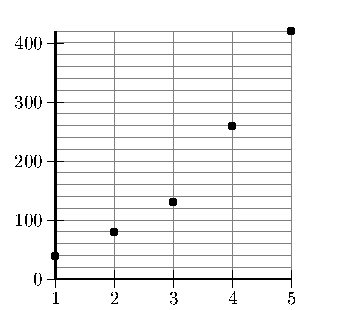
\includegraphics[scale=0.8]{figexo2.pdf}
\end{center}
\item Compléter dans le tableau la ligne indiquant $ z_{i}=\log y_{i} $. \textit{(arrondir à $0,01$ près)}
\item Représenter le nuage de points $ B_{i}(x_{i},z_{i}) $ dans le repère ci-dessous :\\
\begin{center}
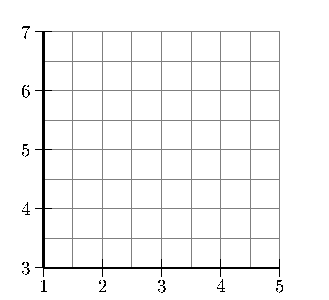
\includegraphics[scale=0.8]{figexo3.pdf}
\end{center}
\item Donner une équation de la droite de régression de $ z $ en $ x $ obtenue par la méthode des moindres carrés et tracer cette droite dans le repère. \textit{($ a $ et $ b $ seront arrondis à $0,001$ près)}
\item En déduire l'expression de $ y $ en fonction de $ x $ en suivant ce modèle. \textit{(on écrira $ y $ sous la forme $ A\times 10^{Bx} $ en arrondissant $ A $ à $ 0,001 $  près)}
\item Selon ce modèle, quel serait le nombre d'abonnés en 2022 ? \textit{(donner le résultat au millier près)}
\end{enumerate}
\end{exocor}

\newpage
\section*{Corrigés}

\begin{corrige}
Dans chaque cas, on donne les cinq premiers termes d'une suite $\left(u_{n}\right)$. Trouver les deux termes suivants possibles $u_{5}$ et $u_{6}$ de manière logique.


\begin{enumerate}
\begin{multicols}{5}
\item $u_{0}=-3$

$u_{1}=1$

$u_{2}=5$

$u_{3}=9$

$u_{4}=13$

$u_5=17$

$u_6=21$

\item $u_{0}=1$

$u_{1}=3$

$u_{2}=9$

$u_{3}=27$

$u_{4}=81$

$u_5=243$

$u_6=729$

\item $u_{0}=7$

$u_{1}=12$

$u_{2}=19$

$u_{3}=28$

$u_{4}=39$

$u_5=52$

$u_6=67$

\item $u_{0}=-1$

$u_{1}=2$

$u_{2}=-4$

$u_{3}=8$

$u_{4}=-16$

$u_{5}=32$

$u_{6}=-64$

\item $u_{0}=\frac{1}{2}$

$u_{1}=\frac{3}{5}$

$u_{2}=\frac{5}{8}$

$u_{3}=\frac{7}{11}$

$u_{4}=\frac{9}{14}$

$u_{5}=\frac{11}{17}$

$u_{6}=\frac{13}{20}$
\end{multicols}
\end{enumerate}
\end{corrige}



\begin{corrige}
Déterminer la moyenne arithmétique des réels $a$ et $b$ dans chacun des cas suivants :
\begin{enumerate}
\begin{multicols}{3}
\item $a=5$ et $b=15$.\\
$m=10$
\item $a=\frac{1}{3}$ et $b=-\frac{3}{7}$.\\
$m=\frac{-1}{21}$
\item $a=105$ et $b=-205$.\\
$m=-50$
\end{multicols}
\end{enumerate}
\end{corrige}

\begin{corrige}


\begin{enumerate}
\item Soit $\left(u_{n}\right)$ la suite arithmétique de raison 3 et de premier terme $u_{0}=2$.

Calculer $u_{1}, u_{2}, u_{3}, u_{4}$ et $u_{6}$.

$$u_1=5; \; u_2=8; \; u_3=11; \; u_4=14 \; u_6=20$$


\item Soit $\left(\nu_{n}\right)$ la suite arithmétique de raison -8 et de premier terme $v_{0}=28$.

Calculer $v_{1}, v_{2}, v_{3}, v_{4}$ et $v_{6}$.

$$v_1=20; \; v_2=12; \; v_3=4; \; v_4=-4 \; v_6=-12$$

\item Soit $\left(w_{n}\right)$ la suite arithmétique de raison 3 et de premier terme $w_{0}=\frac{1}{7}$.

Calculer $w_{1}, w_{2}, w_{3}, w_{4}$ et $w_{6}$.

$$w_1=\dfrac{22}{7}; \; w_2=\dfrac{43}{7}; \; w_3=\dfrac{64}{7}; \; w_4=\dfrac{85}{7} \; w_6=\dfrac{127}{7}$$
\end{enumerate}
\end{corrige}


\begin{corrige}
\begin{enumerate}
\item Soit $\left(u_{n}\right)$ la suite arithmétique de raison $r=-2$ et de premier terme $u_{0}=7$.

Exprimer $u_{n}$ en fonction de $n$ puis calculer $u_{10}$ et $u_{100}$.

$$u_n=7 \times (-2)^n, \;\;\; u_{10}=7168, \;\;\; u_{100}=7\times 2^{100} \approx 8,87 \times 10^{30}$$

\item Soit $\left(v_{n}\right)$ une suite arithmétique telle que $v_{2}=7$ et $v_{6}=9$.

Calculer sa raison $r$ puis son premier terme $v_{0}$. 

$$v_6=v_2+(6-2)r \Longleftrightarrow r=\dfrac{v_6-v_2}{4}=\dfrac{1}{2}=0,5$$

\end{enumerate}
\end{corrige}



\begin{corrige}
Dans chaque cas, on donne les premiers termes $u_{0}, u_{1}, u_{2}, u_{3}$ et $u_{4}$ d'une suite $\left(u_{n}\right)$.

Dans quel cas peut-elle être arithmétique?

\begin{enumerate}
\item $0 ; 1 ; 4 ; 9 ; 16$.\\
La suite ne peut pas être arithmétique car les écarts sont non constants à savoir 1;3;...

\item $28 ; 21 ; 14 ; 7 ; 0$.\\
La suite peut être arithmétique car les écarts sont constants à savoir -7.

\item $5,2 ; 5,6 ; 6 ; 6,4 ; 6,8$.\\
La suite peut être arithmétique car les écarts sont constants à savoir 0,4.

\end{enumerate}
\end{corrige}


\begin{corrige}
\begin{enumerate}
\item Calculer la somme des 500 premiers entiers naturels non nuls.\\
Il s'agit d'une somme dont les termes forment le début d'une suite arithmétiques\\

Nombre de terme est de 500, premier terme est égal à 1 et le dernier terme est égal à 500, par suite $S=500\dfrac{1+500}{2}=125250$

\item Calculer la somme des entiers de 35 à 150.\\
La somme des entiers jusqu'à 150 est de 11325.
La somme des entiers jusqu'à 34 est de 595. 
Donc la somme des entiers de 34 jusqu'à 150 est de 10730.\\

Autre technique: Il y a 150-35+1=116 termes donc la somme est de $116\times \dfrac{35+150}{2} = 10730$ 
 
\end{enumerate}
\end{corrige}


\begin{corrige}

Soit $\left(u_{n}\right)$ la suite arithmétique de raison 3 et de premier terme $u_{0}=5$.

\begin{enumerate}
\item Exprimer $u_{n}$ en fonction de $n$ puis en déduire $u_{15}$.\\
$u_n=5+3n$ donc on a $u_{15}=50$
\item Calculer $S=u_{0}+u_{1}+\ldots+u_{15}$.\\
Il y a $15-0+1=16$ termes donc $S=16\times\dfrac{5+50}{2}=440$
\end{enumerate}
\end{corrige}

\begin{corrige}
Soit $\left(u_{n}\right)$ la suite arithmétique telle que $u_{3}=5$ et $u_{14}=39$.

\begin{enumerate}
\item Déterminer le nombre de termes de $u_{3}$ à $u_{14}$.\\
Il y a 14-3+1 termes soit 12 termes.
\item Calculer $S=u_{3}+u_{4}+\ldots+u_{14}$. \\
D'après ce que l'on sait $S=12\dfrac{5+39}{2}=264$.
\end{enumerate}
\end{corrige}


\begin{corrige}
Une personne qui n'a aucune pratique sportive décide au cours d'un mois de 30 jours de faire chaque jour 5 minutes de sport de plus que le jour précédent.

On modélise cette situation par une suite $\left(t_{n}\right)$ où $t_{n}$ est le temps consacré par cette personne à faire du sport le $n$-ième jour de ce mois.

\begin{enumerate}
\item Déterminer $t_{1}$ et $t_{2}$.\\
$$t_1=5, \;\;\; t_2=10$$

\item Déterminer la nature de la suite $\left(t_{n}\right)$.\\
La suite est arithmétique, de raison $5$ et de premier terme 5.

\item Exprimer $t_{n}$ en fonction de $n$.
$$t_n=t_1 + 5(n-1)= 5n$$

\item Déterminer le temps consacré à faire du sport le trentième jour.
$t_30=150$ Soit deux heures et demi de sport.

\item Calculer $S=t_{1}+t_{2}+\ldots+t_{30}$.

$S=30\times\dfrac{5+150}{2}=2325$

\item Interpréter ce dernier résultat.\\

Durant ce mois, cette personne aura pratiquer 2325 minutes de sport, soit 38 heures et 45 minutes.
\end{enumerate}
\end{corrige}



\begin{corrige}
Un apiculteur s'inquiète pour sa population d'abeilles.

Il l'évalue la première année à 10 000, la deuxième à 9 250, et la troisième à 8200.

Peut-il modéliser l'évolution du nombre d'abeilles par une suite arithmétique? \\

L'écart entre la première et la seconde année est 750 et l'écart entre la seconde et la troisième est de 1050. L'écart étant non constant il ne peut pas modéliser l'évolution du nombre d'abeilles par une suite arithmétique.
\end{corrige}


\begin{corrige}
Dans une station service lors des trois derniers mois de l'année 2019, le prix du gasoil a évolué de la manière suivante :

\begin{center}
\begin{tabular}{|l|c|c|c|}
\hline Mois & Octobre & Novembre & Décembre \\
\hline Prix (en euros) & 1,491 & 1,503 & 1,515 \\
\hline
\end{tabular}
\end{center}

L'évolution de ce prix peut-elle être modélisée par une suite arithmétique? Si oui, laquelle?\\

L'écart est constant d'un mois à un autre et est de 0,012. On peut modéliser cela par une suite arithmétique de premier terme 1,491 et de raison 0,012.

\end{corrige}


\begin{corrige}

On place un capital de $1250 €$ à intérêts simples au taux annuel de $6 \%$. Cela signifie que les intérêts produits chaque année sont égaux à $6 \%$ de $1250 €$.

On désigne par $I$ les intérêts produits chaque année et par $C_{n}$ la somme disponible au bout de $n$ années. On a donc : $C_{0}=1250$.

\begin{enumerate}
\item Calculer $I$.\\

$I=1250 \times \dfrac{6}{100}=75$

\item Calculer $C_{1}, C_{2}$ et $C_{3}$.\\

$$C_0=1250, \;\;\; C_1=1325, \;\;\; C_2=1400, \;\;\; C_3=1475$$

\item Montrer que $\left(C_{n}\right)$ est une suite arithmétique. Quel est son premier terme? Quelle est la raison?\\

$C_{n+1}-C_n=75$ Donc $(C_n)$ est une suite arithmétique de premier terme $1250$ et de raison $75$. 

\item Exprimer $C_{n}$ en fonction de $n$.\\

$C_n=1250+75n$

\item Calculer la somme disponible au bout de 5 ans.

$C_5=1625$, la somme disponible est de 1625 euros au bout de 5 ans.

\item Au bout de combien d'années la somme disponible dépasse-t-elle $2000 €$ ?
On cherche $n$ tel que 
$$C_n\geq 2000 \Longleftrightarrow 75n \geq 750 \Longleftrightarrow  n \geq 10$$ 

\end{enumerate}
\end{corrige}



\begin{corrige}
La cloche d'une église sonne toutes les heures : 1 coup à 1 h00 et à 13h00; 2 coups à 2 h00 et à $14 \mathrm{~h} 00 ; \ldots ; 12$ coups à midi et à minuit. Un villageois se plaint du bruit.

Pour tout entier naturel $n$ non nul, on note $u_{n}$ le nombre de coups à la $n$-ième heure.

Combien de tintements le villageois entend-il en une journée?\\

$$2(1+2+3+\cdots+12)=2 \times 12 \dfrac{1+12}{2} =24 \dfrac{13}{2} =156$$

Le villageois entend 156 coups de cloche en une journée


\end{corrige}



\begin{corrige}
Cédric s'est inscrit au marathon de Paris et il souhaite organiser sa préparation.

Dans son programme d'entraînement hebdomadaire, il prévoit une séance unique.

Quatre mois avant le départ (on considèrera que cela revient à 16 semaines), lors de sa première semaine de préparation, il court 15 kilomètres. Chaque semaine, il augmente la distance parcourue de 1,5 kilomètre.

Pour tout entier naturel $n$ non nul, on note $u_{n}$ la distance parcourue pendant la séance de la $n$-ième heure.

\begin{enumerate}
\item Préciser $u_{1}, u_{2}$ et $u_{3}$.\\

$$u_1=15, \;\;\; u_2=16,5, \;\;\; u_3=18 $$


\item Déterminer la nature de la suite $\left(u_{n}\right)$.\\

La suite est arithmétique, car l'écart est constant de 1,5.

\item Pensez-vous que Cédric sera prêt pour le marathon de Paris? \\ 

$16\times 1,5=24$ cela ajouté à 15 (=39) ne semble pas suffisant pour arrivé à 42km. 

\item Quelle distance aura-t-il parcourue pendant ses quatre mois d'entraînement?

Il a parcourut $15+16,5+\cdots+39= 16 \dfrac{15+39}{2} =216$ km
 
\end{enumerate}
\end{corrige}



\begin{corrige}
Dans une ville, le prix du $\mathrm{m}^{3}$ d'eau a augmenté de la façon suivante : il coûtait 3,20 euros le $1^{\text {er }}$ janvier 2018, 3,36 euros le $1^{\text {er }}$ janvier 2019 et 3,55 euros le $1^{\text {er }}$ janvier 2020.

Peut-on modéliser l'évolution du prix du $\mathrm{m}^{3}$ d'eau par une suite géométrique? \\

$\dfrac{3,36}{3,20}=1,05$ 
$\dfrac{3,55}{3,36}\approx 1,056$

On ne peut modéliser cela par une suite géométrique car il y aurait une erreur. L'idée serait de mesurer l'erreur pour savoir si elle est significative mais ceci est une autre question.
\end{corrige}


\begin{corrige}

Dans un laboratoire, on introduit initialement $1000 \mathrm{~g}$ de bactéries dans une cuve de milieu nutritif. Le jour suivant, la masse de bactéries est de $1150 \mathrm{~g}$ et le troisième jour de 1 322,5 g.

L'évolution de la masse de bactéries peut-elle être modélisée par une suite géométrique?

$$\dfrac{1150}{1000} =1,15, \;\;\; \dfrac{1322,5}{1150}=1,15$$

On peut modéliser cela par une suite géométrique car les rapports sont constants.
\end{corrige}



\begin{corrige}
\begin{enumerate}
\item Quels sont les coefficients multiplicateurs associés à une hausse de $20 \%$ et à une hausse de $15 \%$ ?\\

$1,2$ et $1,15$ respectivement.

\item Déterminer la moyenne géométrique de 1,2 et 1,15 .\\

$$\sqrt{1,2 \times 1,15}\approx 1,1747$$


\item En déduire l'évolution moyenne associée à deux hausses successives, une première de $20 \%$ et une deuxième de $15 \%$.\\

L'évolution moyenne associé à ces deux évolutions est une augmentation de $17,47\%$.
\end{enumerate}
\end{corrige}


\begin{corrige}
\begin{enumerate}

\item Quels sont les coefficients multiplicateurs associés à une baisse de $30 \%$ et à une baisse de $25 \% $?\\

$1-\dfrac{30}{100}=0,7$ et $1-\dfrac{25}{100}=0,75$.

\item Déterminer la moyenne géométrique de 0,7 et 0,75 .\\

$\sqrt{0,7 \times 0,75}\approx 0,7246 =1-\dfrac{27,54}{100}$

\item En déduire l'évolution moyenne associée à deux baisses successives, une première de $30 \%$ et une deuxième de $25 \%$.\\

L'évolution moyenne associé à ces deux évolutions est une diminution de $27,54\%$.

\end{enumerate}
\end{corrige}


\begin{corrige}
Chaque somme $S$ est la somme de termes successifs d'une suite géométrique $\left(u_{n}\right)$. Calculer $S$.

\begin{enumerate}
\item $S=1+2+4+\ldots+2048$.

$$S=\dfrac{1-2^{12}}{1-2}=2^{12}-1$$

\item $S=3+\frac{3}{2}+\frac{3}{4}+\ldots+\frac{3}{8192}$.

$$S=3\times \dfrac{1-(\frac{1}{2})^{14}}{1-\frac{1}{2}}=6(1-(\dfrac{1}{2})^{14})$$

\item $S=2+6+18+\ldots+13122$.

$$S=2 \times (\dfrac{1-3^{9}}{1-3})=3^9-1$$
\end{enumerate}
\end{corrige}



\begin{corrige}
Une entreprise place un capital de 10000 euros à intérêts composés au taux annuel de $3 \%$. Cela signifie que chaque année, le capital augmente de $3 \%$.

On note $C_{n}$ la valeur acquise par le capital au bout de $n$ années.
\begin{enumerate}
 
\item Calculer $C_{1}$ et $C_{2}$.

$C_1=10300$ et $C_2=10609$

\item Indiquer la nature de la suite des capitaux $\left(C_{n}\right)$.

La suite des capitaux forment une suite géométrique de premier terme 10000 et de raison 1,03.

\item Exprimer le terme général $C_{n}$ en fonction de $n$.

$$C_n=10000\times 1,03^n$$ 

\item Calculer la valeur acquise par le capital au bout de 10 ans.\\

La valeur acquise au bout de 10 ans sera de $C_{10}\approx 13439,16$


 \end{enumerate} 
\end{corrige}


\begin{corrige}
En 2018, les dépenses de fonctionnement d'une entreprise s'élevaient à 12500 euros. Depuis, elles diminuent de 5,5\% par an.

Le responsable veut savoir à partir de quelle année les dépenses de fonctionnement seront inférieures à 10000 euros si la baisse se poursuit avec la même évolution annuelle.

Pour tout entier naturel $n$, on note $d_{n}$ les dépenses de fonctionnement l'année $2018+n$.

\begin{enumerate}
\item Préciser $d_{0}, d_{1}$ et $d_{2}$.\\

$d_0=12500$; $d_1=11812,5$; et $d_2\approx 11162.81$

\item Déterminer la nature de la suite $\left(d_{n}\right)$.\\

La suite $(d_n)$ est géométrique de premier terme $12500$ et de raison $1-\dfrac{5,5}{100}$.

\item Exprimer le terme général $d_{n}$ en fonction de $n$.\\

$$d_n=12500\times (1-\dfrac{5,5}{100})^n$$

\item Conclure en utilisant une calculatrice.\\

A partir de $n\geq 4$ $d_n\leq 10000$ les dépenses de fonctionnement de l'entreprise seront inférieurs à 10000 euros dans 4 ans.

\end{enumerate}
\end{corrige}



\begin{corrige}
Un atelier fabrique 250 paires de lunettes par semaine. Au $1^{\text {er }}$ janvier 2019, il reçoit une commande de 7500 pièces pour début juin. Le chef d'atelier compte réaliser cette commande en 24 semaines.

\begin{enumerate}
\item Ce délai est-il suffisant? Justifier la réponse.

$24 \times 250 =6000 < 7500$

\item Le chef d'atelier décide d'augmenter la production de $5 \%$ par semaine. On note $u_{n}$ le nombre de paires de lunettes produites la $n$-ième semaine.

\begin{enumerate}
\item Calculer $u_{1}$ et $u_{2}$.

$u_1 \approx 262$ et $u_2\approx 275$

\item Déterminer la nature de la suite $\left(u_{n}\right)$.

La suite $u_n$ est géométrique de raison 1,05 et de premier terme 250

\item Exprimer le terme général $u_{n}$ en fonction de $n$.\\

$$u_n=250\times 1,05^n$$
\end{enumerate}

\item Conclure.

$$250+262,5+\cdots+806,27..=250(\dfrac{1-(1,05)^{24}}{1-1,05}=5000(1,05^{24}-1)\approx 11125 > 7500$$

La commande sera bien honorée.
\end{enumerate}
\end{corrige}


\begin{corrige}

Un jour donné, la pression atmosphérique à l'altitude 0 est égale à 1000 hectopascals (hPa) et diminue de $1 \%$ pour une élévation d'altitude de 100 mètres.

Pour tout entier naturel $n$, on note $u_{n}$ la pression à $n$ centaines de mètres d'altitude.

\begin{enumerate}
\item Déterminer la pression atmosphérique à $100 \mathrm{~m}$ et à $200 \mathrm{~m}$ d'altitude.

$u_1=990$ et $u_2=980,1$.

\item Quelle est la nature de la suite $\left(u_{n}\right)$ ?

La suite $(u_n)$ est une suite géométrique de raison 0,99 et de premier terme 1000.

\item Exprimer $u_{n}$ en fonction de $n$.

$$u_n= 1000 \times 0,99^n$$
 
\item En déduire la pression atmosphérique au sommet du Mont-Blanc à $4800 \mathrm{~m}$ ce jour-là.

La pression au sommet du Mont-Blanc est de $u_48\approx 617$ hPa.

\end{enumerate}

\end{corrige}

\begin{corrige}
Étienne vient d'acheter un lave-linge très perfectionné à 1500 euros qu'il décide d'assurer. En cas de défaillance, l'assureur rembourse l'appareil mais il applique une décote de $12 \%$ par an sur la valeur de l'appareil. On note $a_{n}$ la valeur remboursée du lave-linge la $n$-ième année.

\begin{enumerate}
\item Calculer $a_{1}$ et $a_{2}$.

$a_1=1320$ et $a_2=1161,6$

\item Quelle est la nature de la suite $\left(a_{n}\right)$ ?

La suite $(a_n)$ est une suite géométrique de raison 0,88 et de premier terme 1500

\item Exprimer $a_{n}$ en fonction de $n$.

$$a_n=1500\times (1-\dfrac{12}{100})^n$$

\item A partir de quelle année la valeur remboursée sera-t-elle inférieure à 100 euros? \\

A partir de $n \geq 22$ $a_n \leq 100$, autrement dit dans 22 ans la somme remboursé sera inférieur à 100 euros.  


\end{enumerate}
\end{corrige}

\begin{corrige}

\textbf{Partie A}

En France depuis 2016, les ventes de véhicules hybrides ont fortement augmenté. Le tableau ci-dessous donne le nombre de véhicules hybrides vendus en France par année :

\begin{center}
\begin{tabular}{|l|c|c|c|}
\hline Année & 2016 & 2017 & 2018 \\
\hline Nombre de véhicules & 7420 & 11010 & 15350 \\
\hline
\end{tabular}
\end{center}

\begin{enumerate}
\item Déterminer le pourcentage d'évolution entre 2016 et 2017, puis entre 2017 et 2018.\\

le pourcentage d'évolution entre 2016 et 2017 est de $\dfrac{11010-7420}{7420}\times 100 \approx 48,38\%$, puis entre 2017 et 2018 le pourcentage d'évolution est de $\dfrac{15350-11010}{11010}\times 100 \approx 39,42\%$

\item Déterminer la moyenne géométrique de 1,48 et 1,39 .\\

$$\sqrt{1,48 \times 1,39}\approx 1,4343$$


\item Quel est le taux moyen annuel d'évolution entre 2016 et 2018 ?\\

 le taux moyen annuel d'évolution entre 2016 et 2018 est d'environ $43,43\%$
\end{enumerate}

\textbf{Partie B}

On suppose qu'à partir de 2018, les ventes de voitures hybrides augmentent de $43 \%$ par an et que cette évolution va se poursuivre.

On modélise par la suite $\left(u_{n}\right)$ l'évolution des ventes où la partie entière de $u_{n}$ représente le nombre de voitures hybrides vendues au cours de l'année $2018+n$.

\begin{enumerate}
\item 
\begin{enumerate}
\item Que vaut $u_{0}$ ?
$u_0=15350$
\item Calculer $u_{1}$ et $u_{2}$.
$u_1=21950.5$ et $u_2=31389,215$.
\end{enumerate}

\item Quelle est la nature de la suite $\left(u_{n}\right)$ ?\\

La suite $(u_n)$ est une suite géométrique de raison 1,43 et de premier terme 15350.

\item Exprimer $u_{n}$ en fonction de $n$.

$$u_n=15350 \times 1,43^n$$

\item Selon ce modèle, combien de voitures hybrides seront vendues en 2023 ?

$$u_5= 15350 \times 1,43^5 \approx 91788$$ 

Arrondi à la partie entière le nombre de voiture hybrides vendues sera de 91788 en 2023.
\end{enumerate}
\end{corrige}



\begin{corrige}
Pour un emploi où elle compte rester 15 ans, Bahiya se voit proposer deux contrats de travail :

\begin{itemize}
\item Contrat 1 : 21000 euros de salaire annuel net et une augmentation annuelle de 1000 euros;

\item Contrat 2 : 18000 euros de salaire annuel net et une augmentation annuelle de $8 \%$.
\end{itemize}

\begin{enumerate}
\item On commence par étudier le contrat 1 .

\begin{enumerate}
\item On note $u_{n}$ la valeur du salaire annuel de Bahiya la $n$-ième année. Déterminer $u_{1}, u_{2}$ et $u_{3}$.\\

$u_1=21000, \;\;\; u_2=22000, \;\;\; u_3=23000$

\item Quelle est la nature de la suite $\left(u_{n}\right)$ ?\\

La suite $(u_n)$ est une suite arithmétique de raison 1000 et de premier terme 21000.

\item Exprimer $u_{n}$ en fonction de $n$.\\ 

$$u_n=21000+1000(n-1)$$

\item Calculer $u_{15}$.

$$u_{15}=35000$$
\end{enumerate}

\item On étudie maintenant le contrat 2.

\begin{enumerate}
\item On note $v_{n}$ la valeur du salaire annuel de Bahiya la $n$-ième année. Déterminer $v_{1}, v_{2}$ et $v_{3}$.\\

$v_1=18000, \;\;\; v_2=19440, \;\;\; v_3=20995,2$

\item Quelle est la nature de la suite $\left(v_{n}\right)$ ?\\

La suite $(v_n)$ est une suite arithmétique de raison 1,08 et de premier terme 18000.

\item Exprimer $v_{n}$ en fonction de $n$.\\

$$v_n=18000 \times 1,08^{n-1}$$

\item Calculer $v_{15}$.\\

$v_{15}=18000 \times 1,08^{14} \approx 52869,49$
\end{enumerate}

\item Comparer les deux contrats sur le long terme. \\

Sur le long termes il est plus avantageux pour le salarié de prendre le contrat 2.
\end{enumerate}
\end{corrige}



\begin{corrige}
L'entreprise Iron SA exploite un filon de minerai de fer depuis 1950.

La première année d'extraction l'entreprise a récupéré 20000 tonnes de fer. Cependant depuis 1950, en raison de difficultés croissantes d'extraction, de l'appauvrissement du filon, les quantités extraites diminuent de $1 \%$ par an.

On appelle $T_{n}$ le nombre de tonnes extraites l'année $(1950+n)$. On a donc $T_{0}=20000$.

Les résultats seront arrondis à la tonne.
\begin{enumerate}

\item Justifier que $T_{1}=19800$ puis calculer $T_{2}$ et $T_{3}$.\\

$$T_1=20000 \times 0,99 =19800, \;\;\; T_2=19602, \;\;\; T_3=194055,98$$
\item Exprimer $T_{n+1}$ en fonction de $T_{n}$.

$$T_{n+1}=T_n \times 0,99$$

\item Quelle est la nature de la suite $\left(T_{n}\right)$ ? En déduire l'expression de $T_{n}$ en fonction de $n$.

La suite $(T_n)$ est une suite géométrique de raison 0,99 et de premier terme 20000, $T_n=20000 \times 0,99^n$.


\item Quelle est la quantité extraite en 2008?\\

$T_{58}\approx 1116$

La quantité extraite en 2008 est de 1116 tonnes environ.

\item Montrer que la quantité totale extraite entre l'année 1950 et l'année $(1950+n)$ est :

$$
S_{n}=2000000 \times\left(1-0,99^{n+1}\right)
$$

Il s'agit d'une somme dont les termes sont géométrique il  y a bien $n$ terme et diviser par $1-0,99$ revient à multiplier par 100 d'où les 2 000 000.

6. En 1950, les géologues estimaient que ce filon recelait 1000000 tonnes de métal. En quelle année, théoriquement, le filon sera-t-il épuisé?\\

Théoriquement cela arrivera pendant la 68 ième année pour extraire tous le filon et donc en 2018.
\end{enumerate}
\end{corrige}

\begin{corrige}
Cet exercice est composé de deux parties indépendantes l'une de l'autre.

\textbf{Partie A - Les économies}\\

Afin de se constituer un capital, un épargnant place 1000 euros sur un compte non rémunéré et, chaque mois, verse 75 euros sur ce compte.

On note $u_{n}$ le montant en euros du capital accumulé au bout de $n$ mois. Ainsi $u_{0}=1000$.

\begin{enumerate}
\item Calculer $u_{1}, u_{2}$ et $u_{3}$.

$$u_1=1075; \;\;\; u_2=1150, \;\;\; u_3=1225$$

\item Déterminer la nature de la suite $\left(u_{n}\right)$ en justifiant la réponse.\\

La suite $(u_n)$ est une suite arithmétique car l'écart est constant de raison 75 et de premier terme 1000.


\item En déduire l'expression de $u_{n}$ en fonction de $n$.
Au bout de combien de temps le capital accumulé est-il supérieur à 3500 euros? Justifier la réponse.

$$u_n=1000+75n$$

$$u_n\geq 3500 \Longleftrightarrow 75n \geq 2500 \Longleftrightarrow n\geq 34$$

Au bout de 34 ans, le capital accumuler sera serait supérieur à 3500 euros.


\end{enumerate}

\textbf{Partie B - Les dépenses}\\

Cet épargnant doit surveiller ses dépenses. En janvier 2014 il a dépensé $660 €$ et, jusqu'à présent, ses dépenses ont augmenté chaque mois de $4 \%$. On suppose que cette évolution va se poursuivre à l'avenir.

Cette évolution conduit à modéliser le montant en euros des dépenses mensuelles au cours du $n$-ième mois après janvier 2014 par le terme $v_{n}$ d'une suite géométrique. Ainsi $v_{0}=660$.

Dans cette partie, les résultats seront arrondis au centime d'euro.

\begin{enumerate}
\item Justifier que $v_{1}=1,04 v_{0}$. Calculer $v_{3}$ et interpréter le résultat.

Ici les dépense du premier mois sont 4\% supérieur à 660 euros. soit $1,04 \times 660$.  $$v_3=1,04 \times v_2 =1,04 \times 1,04 \times v_1 =1,04 \times 1,04 \times 1,04 v_0 = 1,04^3 v_0=742$$

\item Calculer le montant des dépenses au mois de décembre 2014.

$v_12=(1,04)^12 660 \approx 1056,68$

Les dépenses seront de 1056,68 euros au mois de décembre 2014.

\item Selon ce modèle, quand l'épargnant devrait-il doubler ses dépenses par rapport à janvier 2014 ? \\

$$(1,04)^n 660 \geq 1320 \Longleftrightarrow (1,04)^n \geq 2  \Longleftrightarrow n \geq 18$$

Au bout de 18 mois, soit en juin 2015. 

\end{enumerate}
\end{corrige}

\begin{corrige}
Deux coureurs cyclistes, Ugo et Vivien, ont programmé un entraînement hebdomadaire afin de se préparer à une course qui aura lieu dans quelques mois. Leur objectif est de parcourir chacun une distance totale de $1500 \mathrm{~km}$ pendant leur période d'entraînement de 20 semaines.

Ugo commence son entraînement en parcourant $40 \mathrm{~km}$ la première semaine et prévoit d'augmenter cette distance de $5 \mathrm{~km}$ par semaine. Vivien commence son entraînement en parcourant $30 \mathrm{~km}$ la première semaine et prévoit d'augmenter cette distance de $10 \%$ par semaine.

On note $u_{n}$ la distance, en kilomètres, parcourue par Ugo la $n^{\text {ième }}$ semaine. On a ainsi $u_{1}=40$. On note $v_{n}$ la distance, en kilomètres, parcourue par Vivien la $n^{\text {ième }}$ semaine. On a ainsi $v_{1}=30$.

\textbf{Partie A - L'entraînement d'Ugo}

\begin{enumerate}
\item Calculer les distances parcourues par Ugo au cours des deuxième et troisième semaines d'entraînement.\\

$$u_2=45, \;\;\; u_3=50$$

\item Quelle est la nature de la suite $\left(u_{n}\right)$ ? Préciser sa raison.\\

$(u_n)$ est une suite arithmétique de raison 5 et de premier terme 40.

\item Montrer que, pour tout $n \geqslant 1, u_{n}=35+5 n$.

$$u_n=u_1+(n-1)\times 5=40+5n-5=35+5n$$

\end{enumerate}

\textbf{Partie B - L'entraînement de Vivien}

\begin{enumerate}
\item Quelle est la nature de la suite $\left(v_{n}\right)$ ? Justifier la réponse.

La nature de $(v_n)$ est une suite géométrique car elle augmente de 10\% par semaine ce qui revient à multiplier par un même nombre à savoir la raison qui est de $1,1=q$. 

\item Montrer que, pour tout $n \geqslant 1, v_{n}=30 \times 1,1^{n-1}$.\\

Pour $n\geq1$,
$$v_n=v_1 \times q^{n-1} = 30 \times 1,1^{n-1}$$

\item Calculer $v_{8}$. On arrondira le résultat au dixième.\\

$$v_8\approx 58,5$$

\end{enumerate}

\textbf{Partie C - Comparaison des deux entraînements}

\begin{enumerate}
\item Vivien est persuadé qu'il y aura une semaine où il parcourra une distance supérieure à celle parcourue par Ugo. Vivien a-t-il raison? On pourra utiliser les PARTIES A et B pour justifier la réponse.\\

Au bout de la 13 ème semaine Vivien dépassera une distance supérieur celle de Ugo. 

$$u_{13} =100, \;\;\; v_{13}\approx 103,56$$

\item À la fin de la $17^{\mathrm{e}}$ semaine, les deux cyclistes se blessent. Ils décident alors de réduire leur entraînement. Ils ne feront plus que $80 \mathrm{~km}$ chacun par semaine à partir de la $18^{\mathrm{e}}$ semaine. Leur objectif sera-t-il atteint?\\

$$S_u=u_1+\cdots+u_{17}+80\times 3=17\times \dfrac{40+125}{2} + 240 = 1600$$ 

$$S_v=v_1+\cdots+v_{17}+ 80 \times 3=30 \times \dfrac{1-1,04^18}{1-1,04} + 240 \approx 1009$$

L'objectif sera atteint pour Ugo mais pas pour Vivien.  

\end{enumerate}

\end{corrige}

\begin{corrige}

Un youtubeur compte 35000 abonnés à sa chaîne au 1er janvier 2019.

Au cours de l'année 2019, il constate que chaque mois, il perd $20 \%$ des anciens abonnés mais qu'il en gagne 500 nouveaux.

Pour $n \geqslant 1$, on note $u_{n}$ le nombre d'abonnés le $1^{\text {er }}$ du $n$-ième mois, le premier mois étant le mois de janvier 2019.

\begin{enumerate}
\item Préciser $u_{1}$.

$u_1=35000$

\item Calculer $u_{2}$ et $u_{3}$. \\

$$u_2=35000 \times 0,8 +500 =28500$$
$$u_3=28500 \times 0,8 +500=23300$$


\item La suite $\left(u_{n}\right)$ est-elle arithmétique? Est-elle géométrique?

Elle n'est pas arithmétique car l'écart n'est pas constant entre les termes (7000 puis 5200).\\
Elle n'est pas géométrique car le rapport n'est pas constant entre les termes (1,2280  et 1,2231  environ).



\item On introduit la suite $\left(v_{n}\right)$ définie pour tout entier $n \geqslant 1$ par $v_{n}=u_{n}-2500$.

\begin{enumerate}
\item Démontrer que la suite $\left(v_{n}\right)$ est une suite géométrique.

Préciser sa raison et son premier terme.\\

$$\dfrac{v_{n+1}}{v_n}=\dfrac{u_{n+1}-2500}{v_n}=\dfrac{u_n \times0,8+500-2500}{v_n}=\dfrac{u_n\times 0,8-2000}{v_n}=\dfrac{0,8(u_n-2500)}{v_n}=\frac{0,8v_n}{v_n}=0,8$$

\item Exprimer $v_{n}$ en fonction de $n$ et en déduire l'expression de $u_{n}$ en fonction de $n$.\\

$$v_n=v_1 \times 0,8^{n-1}=32500 \times 0,8^{n-1}$$
$$u_n=v_n+2500=32500 \times 0,8^{n-1}+2500$$

\item Déterminer le nombre d'abonnés au $1^{\text {er }}$ janvier 2020.\\

$$u_{13} \approx 4287$$

Le nombre d'abonnés sera d'environ 4287 le 
$1^{\text {er }}$ janvier 2020.

\end{enumerate}
\end{enumerate}
\end{corrige}

\begin{corrige}
\begin{enumerate}
\item Non ce n'est pas une probabilité conditionnelle  $\mathbb{P}(P)=0,4$
\item Oui, $\mathbb{P}_P(V)=0,66$
\item Oui, $\mathbb{P}_{\bar{V}}(P)=0,22$
\item Non ce n'est pas une probabilité conditionnelle $\mathbb{P}(\bar{V}\cap\bar{P})$
\end{enumerate}
\end{corrige}

\begin{corrige}
\begin{enumerate}
\item $\mathbb{P}_F(R)=0,25$
\item $\mathbb{P}_H(R)=\dfrac{1}{3}$
\item $\mathbb{P}_R(F)=0,45$
\item $\mathbb{P}_H(\bar{R})=0,67$
\item $\mathbb{P}_{\bar{R}}(F)=0,55$
\end{enumerate}
\end{corrige}

\begin{corrige}
\begin{enumerate}
\item $\mathbb{P}(Q)=0,1$; $\mathbb{P}(R)=0,22$; $\mathbb{P}(Q \cap R)=0,04$
\item $$\mathbb{P}_Q(R)=\dfrac{\mathbb{P}(Q\cap R)}{\mathbb{P}(Q)}=\dfrac{0,04}{0,1}=0,4$$

La probabilité que l'exercice choisi a des questions sur les probabilités sachant que l'exercice choisi est un QCM est de 40\%.

 $$\mathbb{P}_R(Q)=\dfrac{\mathbb{P}(Q\cap R)}{\mathbb{P}(R)}=\dfrac{0,04}{0,22}=0,0088$$
La probabilité que l'exercice choisi est un QCM sachant que l'exercice choisi a des questions sur les probabilités est de 0,88\%.
\end{enumerate}
\end{corrige}

\begin{corrige}
\begin{enumerate}
\item $\mathbb{P}(C)=\dfrac{1296}{2400}$; $\mathbb{P}(O)=\dfrac{2400-1296}{2400}=\dfrac{1104}{2400}$; $\mathbb{P}_O(A)=0,25$; $\mathbb{P}_C(A)=\dfrac{1}{3}$
\item Arbre pondéré
\begin{center}
\begin{tikzpicture}[
    level 1/.style={level distance=3cm, sibling distance=3cm},
    level 2/.style={level distance=3cm, sibling distance=2cm},
    grow=right,
  ]
  \coordinate                   % joli sommet de l'arbre
  child {node {$O$}
    child {node {$\bar{A}$} edge from parent node[below]{$0,75$}}
    child {node {$A$} edge from parent node[above]{$0,25$}}
    edge from parent node[below]{$\dfrac{1104}{2400}$}}
  child{node {$C$}
    child {node {$\bar{A}$} edge from parent node[below]{$\dfrac{2}{3}$}}
    child {node {$A$}  edge from parent node[above]{$\dfrac{1}{3}$}}
    edge from parent node[above]{$\dfrac{1296}{2400}$}};
\end{tikzpicture}
\end{center}

\item $\mathbb{P}_O(\bar{A})=1-\mathbb{P}_O(A)=0,75$; $\mathbb{P}_C(\bar{A})=1-\dfrac{1}{3}$

\end{enumerate}
\end{corrige}


\begin{corrige}
\begin{enumerate}
\item Arbre pondéré
\begin{center}
\begin{tikzpicture}[
    level 1/.style={level distance=3cm, sibling distance=3cm},
    level 2/.style={level distance=3cm, sibling distance=2cm},
    grow=right,
  ]
  \coordinate                   % joli sommet de l'arbre
  child {node {$\bar{B}$}
    child {node {$\bar{S}$} edge from parent node[below]{$0,95$}}
    child {node {$S$} edge from parent node[above]{$0,05$}}
    edge from parent node[below]{$0,3$}}
  child{node {$B$}
    child {node {$\bar{S}$} edge from parent node[below]{$0,2$}}
    child {node {$S$}  edge from parent node[above]{$0,8$}}
    edge from parent node[above]{$0,7$}};
\end{tikzpicture}
\end{center}

\item $\mathbb{P}(B \cap S)=0,7 \times 0,8 =0,56$
\item $\mathbb{P}(\bar{B} \cap S)=0,3 \times 0,05 =0,015$
\item $$\mathbb{P}_S(\bar{B})=\dfrac{\mathbb{P}(S\cap \bar{B})}{\mathbb{P}(S)}=\dfrac{0,015}{\mathbb{P}(S)}$$

De plus, $\mathbb{P}(S)=\mathbb{P}(\bar{B} \cap S)+\mathbb{P}(B \cap S)=0,015 +0,7 \times 0,95=0,015+0,665=0,68$ donc, $\mathbb{P}_S(\bar{B})=\dfrac{0,015}{0,68}\approx 0,022$. La probabilité que le sonar détecte un banc de poisson à tort est de 2,2\%.
 

\end{enumerate}
\end{corrige}

\begin{corrige}
\begin{enumerate}
\item $f$ est strictement croissante sur $\mathbb{R}$ car $k=2>0$.
\item 
\begin{center}
\begin{tabular}{|l|l|l|l|l|l|l|l|l|l|}
\hline$x$ & -2 & $-1,5$ & -1 & $-0,5$ & 0 & 0,5 & 1 & 1,5 & 2 \\
\hline$f(x)$ & $0,25$ & $0.354$ & $0,5$ & $0,707$ & $1$ & $1,414$ & $2$ & $2,828$ & $4$ \\
\hline
\end{tabular}
\end{center}
\end{enumerate}
\end{corrige}

\begin{corrige}
\begin{enumerate}
\item $g$ est strictement décroissante sur $\mathbb{R}$ car $k=0,5>0$.
\item 
\begin{center}
\begin{tabular}{|l|l|l|l|l|l|l|l|l|l|}
\hline$x$ & -2 & $-1,5$ & -1 & $-0,5$ & 0 & 0,5 & 1 & 1,5 & 2 \\
\hline$f(x)$ & $4$ & $2,828$ & $2$ & $1,414$ & $1$ & $0,707$ & $0,5$ & $0,354$ & $0,25$ \\
\hline
\end{tabular}
\end{center}
\end{enumerate}
\end{corrige}

\begin{corrige}
\begin{enumerate}
\item \begin{enumerate}
\item La raison de la suite $u_n$ est $1,004$.
\item $u_n=66,9 \times (1,004)^n$
\end{enumerate}
\item \begin{enumerate}
\item $f(x)=66,9 \times (1,004)^x$
\item 2022: $u_3=f(3)\approx 67,7$ ; 2023: $u_4\approx 68$ ; 2025: $u_6 \approx 68.5$
\end{enumerate}
\end{enumerate}
\end{corrige}

\begin{corrige}

\begin{enumerate}
\item Déterminer le sens de variations des fonctions définies sur $\mathbb{R}$ par :
\begin{enumerate}

\item Strictement décroissante sur $\mathbb{R}$ ($k=-2<0$ et $q=1,4>0$)
\item Strictement décroissante sur $\mathbb{R}$ ($k=9,85>0$ et $q=0,85<1$)
\item Strictement croissante sur $\mathbb{R}$ ($k=0,8>0$ et $q=2,25>1$)

\end{enumerate}

\item Déterminer le sens de variations des fonctions définies sur $\mathbb{R}$ par :
\begin{enumerate}

\item Strictement décroissante sur $\mathbb{R}$ ($k=\dfrac{1}{3}>0$ et $q=\dfrac{4}{5}<1$)
\item Strictement croissante sur $\mathbb{R}$ ($k=2>0$ et $q=\dfrac{5}{4}>1$)
\item Strictement décroissante sur $\mathbb{R}$ ($k=-\dfrac{7}{12}<0$ et $q=\dfrac{2020}{2019}>1$)

\end{enumerate}
\end{enumerate}
\end{corrige}

\begin{corrige}
Avec la calculatrice on trouve que 8 mois et 24 jours il y a approximativement 99,85 milliers de joueurs alors qu'à 8 mois et 25 jours on dépasse les 100 milliers de joueurs. 
\end{corrige}

\begin{corrige}
\begin{enumerate}
\item $P(0)=1013=k$ et $1,12=\dfrac{P(1)}{P(0)}=\dfrac{\cancel{k}\times a^1}{\cancel{k} \times a^0}=a$
\item $P(5,5) \approx 1889 $
\end{enumerate}
\end{corrige}

\begin{corrige}
\begin{enumerate}
\item La température de la tasse à café à la sortie du four à micro onde est de $T(0)=86^{\circ} C$ et au bout de 5 minutes $T(5) \approx 59,38^{\circ} C$
\item On peut dire qu'à partir de 6 minutes d'attente, la personne peut boire son café. 
\item Si le temps s'écoule de manière prolongé alors la température de la tasse à café sera la même que la pièce et semble être de $21^{\circ} C$.
\end{enumerate}
\end{corrige}

\begin{corrige}
Graphiquement , on déduit que $k=2$ en regardant la valeur prise par la fonction en 0.  De plus $f(0,5)=3,5$, donc $3,5=2 \times a^{0,5}$. Par suite $a=(\dfrac{3,5}{2})^2$.
\end{corrige}

\begin{corrige}
\begin{enumerate}
\item Ici $q=1,01>1$ donc $f$ est strictement croissante sur $\mathbb{R}$. 
\item D'après ce qui précède on déduit que l'inéquation est équivalent à $x>3,5$
\end{enumerate}
\end{corrige}

\begin{corrige}
\begin{enumerate}
\item Ici $q=0,33<1$ donc $f$ est strictement décroissante sur $\mathbb{R}$. 
\item D'après ce qui précède on déduit que l'inéquation est équivalent à $x\geq 1,8$
\end{enumerate}
\end{corrige}

\begin{corrige}
L'offre $o$ et la demande $d$ pour un produit (en milliers d'unités) sont modélisées par deux fonctions du prix de vente $x$ (en euros).

Pour tout réel $x \in[0 ; 10]$, on a $o(x)=1,3^{x}-1$ et $d(x)=10 \times 0,8^{x}$.

\begin{enumerate}
\item Calculer $o(2)$ et $d(2)$ et interpréter les résultats. \\
$o(2)=1,3^2-1=0,69$ soit 69 offres et $d(2)=10*0,8^2=6,4$ soit 640 demandes, il y a donc plus de demandes que d'offres.

\item Déterminer le sens de variations des fonctions $o$ et $d$.

$o$ est strictement croissante sur $[0;10]$ et $d$ est strictement décroissante sur $[0;10]$.

\item On donne les représentations graphiques des fonctions $o$ et $d$.

\vspace*{-1cm}\hspace*{3.5cm}\includegraphics[scale=1]{expo.3}\vspace*{1cm}

\begin{enumerate}
\item Donner par lecture graphique le montant de l'offre correspondant à un prix de vente de 5 euros.\\

$o(5)\approx 2,7$ soit 270 offres.

\item Utiliser ce graphique pour trouver le prix d'équilibre, où l'offre est égale à la demande.\\

On constate que le prix à l'équilibre se situe vers $5,35$ euros, soit l'abscisse du point d'intersection ou encore quand $o(x)=d(x)$.

\end{enumerate}

\item Retrouver à l'aide de la calculatrice le prix d'équilibre au centime près.\\

\end{enumerate}
\end{corrige}

\begin{corrige}
Écrire sous la forme d'une seule puissance de 2 :
\begin{enumerate}
\begin{multicols}{4}
\item $a=2^{-1,5}$
\item $b=2^{13,5}$
\item $c=2^{3} \times 2^{2 \times 2}=2^7$
\item $d=\dfrac{2^{5}}{2^2}=2^3$ 
\end{multicols}
\end{enumerate}
\end{corrige}

\begin{corrige}

Simplifier les expressions suivantes puis calculer leur valeur :
\begin{enumerate}
\begin{multicols}{4}
\item $a=5^3=125$
\item $b=2^{-2}=0,25$
\item $c=4^{-1}=0,25$
\item $d=\dfrac{6^{6,8}}{6^{4,8}}=6^2=36$
\end{multicols}
\end{enumerate}
\end{corrige}

\begin{corrige}
Le chiffre d'affaires d'une entreprise a augmenté de $38 \%$ en trois ans.
Calculer l'augmentation annuelle moyenne du chiffre d'affaires à $0,1 \%$ près.\\

$$(1+\dfrac{38}{100})^{\dfrac{1}{3}}\approx 1+\dfrac{11,3}{100}$$

Soit une augmentation annuelle du chiffre d'affaires d'environ $11,3 \%$.

\end{corrige}



\begin{corrige}
La taxe foncière en France a augmenté en moyenne de 21,26\% en cinq ans, de 2008 à 2013.

Déterminer son augmentation annuelle moyenne à $0,1 \%$ près. \\

$$(1+\dfrac{21,26}{100})^{\dfrac{1}{5}}\approx 1+\dfrac{3,9}{100}$$

Soit une augmentation annuelle de la taxe foncière d'environ $3,9 \%$.
\end{corrige}

\begin{corrige}

\begin{enumerate}
\item Résoudre sur l'intervalle $] 0 ;+\infty$ [ les équations suivantes :
\begin{enumerate}
\begin{multicols}{4}
\item $x=4^4=256$
\item $x=3^10$
\item $x=2,5^2=6,25$
\item $x=10^3=1000$
\end{multicols}
Toutes les solutions sont bien dans l'ensemble $]0;+ \infty[$.
\end{enumerate}

\item Résoudre sur l'intervalle $] 0 ;+\infty[$ les équations suivantes :
\begin{enumerate}
\begin{multicols}{4}
\item $x=3^{-5}=\dfrac{1}{243}$
\item $x=2^{-6}=\dfrac{1}{64}$
\item $x=5^{-4}=\dfrac{1}{625}$
\item $x=1,5^{-4}=\dfrac{3}{2}^{-4}=\dfrac{16}{81}$
\end{multicols}
Toutes les solutions sont bien dans l'ensemble $]0;+ \infty[$.
\end{enumerate}
\item Résoudre sur l'intervalle $]0 ;+\infty[$ les inéquations suivantes :

\begin{enumerate}
\begin{multicols}{4}
\item $0<x<25$
\item $x \geqslant 32$
\item $0<x \leqslant 243$
\item $0<x<8$
\end{multicols}
\end{enumerate}
\end{enumerate}
\end{corrige}

\begin{corrige}
\begin{enumerate}
\item 
\begin{enumerate}
\item Calculer le taux mensuel $t_{\mathrm{m}}$ équivalent à un taux annuel $t_{\mathrm{a}}=+6 \%$.\\

$$(1+\dfrac{6}{100})^{\dfrac{1}{12}}$$

\item Calculer le taux journalier $t_{\mathrm{j}}$ équivalent à un taux annuel $t_{\mathrm{a}}=+6 \%$. On considère qu'une année comprend 365 jours.\\

$$(1+\dfrac{6}{100})^{\dfrac{1}{365}}$$

\end{enumerate}

\item Un capital de $10000 €$ est placé à intérêts composés au taux annuel $t_{\mathrm{a}}=+6 \%$.

\begin{enumerate}
\item Quelle est la valeur du capital au bout de 1 an? \\

La valeur du capital sera de $10600=10000\times 1,06$ euros au bout d'un an.


\item Quelle est la valeur du capital au bout de 1 mois? au bout de 3 mois?

La valeur du capital sera d'environ $10049=10000\times (1+\dfrac{6}{100})^{\dfrac{1}{12}}$ euros au bout d'un mois et $10147==10000\times (1+\dfrac{6}{100})^{\dfrac{3}{12}}$ euros au bout de trois mois.


\item Quelle est la valeur du capital au bout de 1 jour? au bout de 45 jours? 

La valeur du capital sera d'environ $10002=10000\times (1+\dfrac{6}{100})^{\dfrac{1}{365}}$ euros au bout d'un jour et $10072=10000\times (1+\dfrac{6}{100})^{\dfrac{3}{12}}$ euros au bout de 45 jours.


\end{enumerate}
\end{enumerate}
\end{corrige}

\begin{corrige}
On modélise la population de la ville de Nohouaire depuis 2010 par la fonction $p$ définie par

$$
p(x)=12 \times 2^{\frac{x}{18}}
$$

où $p(x)$ est la population en milliers d'habitants l'année $2010+x$.

\begin{enumerate}
\item Quelle était la population en 2010 et 2020 ?

$$p(0)=12 \;\;\; p(10)=12 \times 2^\dfrac{10}{18}\approx 17,64$$

Soit une population de 12000 habitant en 2010 et 17640  en 2020.

\item En quelle année, selon ce modèle, la population dépassera-t-elle 20000 habitants.

$$p(13)<20 \;\; p(14)>20$$

A partir de l'année 2024 le nombre d'habitant de Nohouraire dépassera 20000.
 

\item Montrer que : $p(x+18)=2 \times p(x)$. Interpréter ce résultat.

$$p(x+18)=12 \times 2^{\dfrac{x+18}{18}} = 12 \times 2 \times 2^\dfrac{x}{18}= 2\times p(x)$$

Autrement dit, la population double tous les 18 ans, quelque soit l'année de départ.
\end{enumerate}
\end{corrige}

\begin{corrige}

Le nombre d'adhérentes à un club de basket a augmenté lors des trois dernières années de $2,5 \%$, puis de $4,1 \%$, et enfin de $3,8 \%$.

Calculer le taux d'évolution annuel moyen.

$$((1+\dfrac{2,5}{100})(1+\dfrac{4,1}{100})(1+\dfrac{3,8}{100}))^{\dfrac{1}{3}}  \approx 1+\dfrac{3,5}{100}$$

\end{corrige}

\begin{corrige}
\begin{enumerate}
\item Une action baisse de $20 \%$ une année, puis de $80 \%$ l'année suivante.

Quel est le pourcentage de baisse annuel moyen.

$$((1-\dfrac{20}{100})(1-\dfrac{80}{100}))^{\dfrac{1}{2}} = 1 -\dfrac{60}{100}$$

\item Quel est le taux d'évolution moyen correspondant à une hausse de $60 \%$, suivie d'une baisse de $60 \%$.

$$((1+\dfrac{60}{100})(1-\dfrac{60}{100}))^{\dfrac{1}{2}}=1-\dfrac{20}{100}$$
\end{enumerate}
\end{corrige}

\begin{corrige}
Le $1^{\text {er }}$ janvier 2019, on a placé 5000 euros sur un compte avec un rendement annuel de $2 \%$.

Les intérêts produits sont calculés au moment du retrait en tenant compte du nombre exact de jours.

La somme d'argent disponible au bout de $x$ années est donnée par $s(x)=k \times a^{x}$ où $k$ et $a$ sont des réels à déterminer.

\begin{enumerate}
\item Déterminer $k$ et $a$.
$s(0)=k=5000$ et $\dfrac{s(1)}{s(0)}=a=1,02$

\item Quelle somme d'argent sera disponible le 8 avril 2019? Et le 15 novembre 2022?

$$s(4+\dfrac{8}{30})\approx 5441 \;\;\; s(11+\dfrac{15}{30})\approx 6279$$

\item Calculer le taux mensuel de ce placement à $0,01 \%$ près.

$$(1,02)^\dfrac{1}{12}=1+\dfrac{0,17}{100}$$

\item Calculer de deux façons différentes la somme d'argent disponible le $1^{\text {er }}$ juillet 2019. Quel résultat est le plus fiable?

$$5000 \times (1+ \dfrac{0,17}{100})^7 \approx 5059,80$$
$$s(\dfrac{7}{12})\approx 5058,09$$

Le plus fiable reste le second résultat qui n'utilise pas d'approximation.

\end{enumerate}
\end{corrige}

\begin{corrige}
Un site internet comptait 46400 abonnés le $1^{\text {er }}$ septembre 2018 et 51156 abonnés le $1^{\text {er }}$ septembre 2020.

\begin{enumerate}
\item Déterminer le taux de croissance annuel moyen de 2018 à 2020.

$$(\dfrac{51156}{46400})^\dfrac{1}{3}=a$$

\item Le directeur du site suppose que la croissance va se poursuivre au même rythme et décide de modéliser le nombre d'abonnés par une fonction $f$ du type $x \mapsto k \times a^{x}$ où $x$ est le nombre d'années écoulées depuis le $1^{\text {er }}$ septembre 2020.

\begin{enumerate}
\item Déterminer les valeurs de $k$ et $a$.\\

$k=51156$
\item Donner la valeur de $f(-2)$ sans utiliser de calculatrice.\\

$f(-2)=46400$
\item Déterminer, selon ce modèle, le nombre d'abonnés prévus le 25 décembre 2020.\\

$f(12+\dfrac{25}{31})\approx 75590$

\item Déterminer, à l'aide de la calculatrice, à quelle date le nombre d'abonnés dépassera 60000. \\

Le 26 octobre 2024.
\end{enumerate}
\end{enumerate}
\end{corrige}

\begin{corrige}
On prélève du sang sur un patient souffrant d'une infection bactérienne. Les bactéries, trop petites, sont indétectables dans le sang et on les met en culture pendant 24 heures.

\begin{enumerate}
\item On observe une phase de latence de 12 heures pendant laquelle les bactéries s'adaptent au milieu, suivie d'une phase de croissance exponentielle de 12 heures durant laquelle le nombre de bactéries par $\mathrm{mL}$ de sang est modélisé par la fonction $f$ définie sur l'intervalle $[12 ; 24]$ par :

$$
f(x)=0,008 \times 2,8^{x}
$$

\begin{enumerate}
\item Justifier que la fonction $f$ est croissante sur l'intervalle [12; 24].\\

Ici $k=0,008>0$ et $q=2,8>1$, la fonction $f$ est donc strictement croissante sur $\mathbb{R}$ et donc strictement croissante \textit{et donc croissante} sur $[12;24]$ car $[12;24] \subset \mathbb{R}$.

\item Déterminer la concentration de bactéries dans la culture au bout de 2 heures $30$ minutes de croissance exponentielle, puis à la fin de la phase de culture.\\

$$f(14,5)=0,008 \times 2,8^{14,5}\approx \numprint{24371} $$
$$f(24)=0,008 \times 2,8^{24} \approx \numprint{431402581}$$

\end{enumerate}

\item Après 24 heures de culture et ayant détecté une infection au Staphylococcus aureus, on introduit un puissant antibiotique.

On admet que la concentration de bactéries, en milliers de bactéries par mL, est alors modélisée par la fonction $g$ définie sur l'intervalle [24 ; 42] par :

$$
g(x)=-1613 x^{2}+82633 x-622702
$$

\begin{enumerate}
\item Étudier les variations de la fonction $g$.\\

La fonction $g$ est dérivable car polynôme du second degré, 
$$g'(x)=-3226x+82633$$

$$g'(x)>0 \Longleftrightarrow x<\dfrac{82633}{3226} \,(\approx 25,6)$$ 

Autrement dit, $g$ est strictement croissante sur $[24;25,6]$ et strictement décroissante sur $[25,6;42]$.

\item Au bout de combien de minutes après l'introduction de l'antibiotique la population de bactéries commence-t-elle à diminuer?\\

Au bout de $25,6-24$ heures soit environ $1$ heure et $36$ minutes.

\item L'antibiotique est jugé bien dosé s'il tue au moins $99 \%$ des bactéries en 18 heures. Cet antibiotique est-il bien dosé? \\

$$\dfrac{g(24+18)}{g(24)}=\dfrac{2552}{431402}\approx 5,9 \times 10^{-3}=0,0059=\dfrac{0,59}{100}<\dfrac{1}{100}$$

L'antibiotique est donc bien dosé. 

\item Représenter sur un graphique l'évolution de la population de bactéries durant les trois phases : latence, croissance exponentielle, élimination.

\end{enumerate}
\end{enumerate}
\end{corrige}

\begin{corrige}
D'un navire perdu au Nouveau Monde débarque 4 souris. Un an après, les souris, qui se reproduisent de façon exponentielle, sont 34 .

Combien de souris seront présentes deux ans et demi après le débarquement.\\

$$s(t)=P_0\times r^t$$ 
avec, 
$P_0=4 \;\;\; r=\dfrac{s(1)}{s(0)}=\dfrac{34}{4}=\dfrac{17}{2}$
et $t$ exprimé en année
$s(2,5)=4 \times (\dfrac{17}{2})^{2,5}  \approx 842,57$ 
 
Au bout de deux ans et demi, il y aura 842 souris.
\end{corrige}

\begin{corrige}
\begin{enumerate}
\item Les valeurs possibles pour $X$ sont $x_1=2$; $x_2=3$ et $x_3=-6$
\item 
\renewcommand{\arraystretch}{2.5}
\begin{tabular}{|c|c|c|c|}
\hline $x_i$ & 2 & 3 & -6 \\
\hline $\mathbb{P}(X=x_i)$ & $\dfrac{3}{6}$ & $\dfrac{1}{6}$ & $\dfrac{2}{6}$ \\
\hline
\end{tabular}
\item $\mathbb{E}(X)=2 \times \dfrac{3}{6} + 3 \times \dfrac{3}{6} + (-6) \times \dfrac{2}{6}=\dfrac{3}{6}$
\item Le jeu n'est pas équitable car l'espérance du gain n'est pas nulle.
\end{enumerate}
\end{corrige}

\begin{corrige}
\begin{enumerate}
\item 
\renewcommand{\arraystretch}{2.5}
\begin{tabular}{|c|c|c|c|c|c|}
\hline $x_i$ & $100-p$ & $50-p$ & $20-p$ & $10-p$ & $0-p$ \\
\hline $\mathbb{P}(G=x_i)$ & $\dfrac{1}{400}$ & $\dfrac{2}{400}$ & $\dfrac{5}{400}$ & $\dfrac{10}{400}$ & $\dfrac{382}{400}$ \\
\hline
\end{tabular}
\item $$\mathbb{E}(G)=(100-p) \times \dfrac{1}{400} + (50-p) \times \dfrac{2}{400} + (20-p) \times \dfrac{5}{400} + (10-p) \times \dfrac{10}{400} +(0-p) \times \dfrac{382}{400} $$
$$\mathbb{E}(G)=\dfrac{100+ 50\times 2 + 20 \times 5 +10 \times 10 + 0 \times 382}{400} -p$$
$$\mathbb{E}(G)=1-p$$

La personne qui achète un billet peut donc espérer en moyenne gagner \emph{ou perdre} $1$ \euro moins le prix du billet. 


\item Les élèves gagnent de l'argent si le gain est négatif, autrement dit il faut que $p$ soit supérieur à $1$ \euro.

\end{enumerate}
\end{corrige}

\begin{corrige}
\begin{enumerate}
\item $\mathbb{P}(X=1)=0,3$
\item La probabilité que le concessionnaire vende trois véhicules dans la journée est de $1-0,45-0,3-0,15=0,1$
\item $\mathbb{P}(X \geq 1)= 1-\mathbb{P}(X < 1) = 1-0,45=0,55$
\item $\mathbb{E}(X)=0 \times 0,45 + 1 \times 0,3 + 2 \times 0,15 + 3 \times 0,1=0,3+0,3+0,1=0,9$
\end{enumerate}
\end{corrige}


\begin{corrige}
\begin{enumerate}
\item $X$ peut prendre les valeurs $3;2;$ et $1,5$.
\item
\begin{tabular}{|c|c|c|c|}
\hline$x_{i}$ & 3 & 2 & 1,5  \\
\hline$\mathbb{P}\left(X=x_{i}\right)$ & 0,8 & 0,15 & 0,05 \\
\hline
\end{tabular}

\item $$\mathbb{E}(X)=3 \times 0,8 + 2 \times 0,15 + 1,5 \times 0,05=2,4+0,3+0,225=2,925$$ L'entreprise peut donc espérer vendre une brioche à 2,925 \euro en moyenne.
\end{enumerate}
\end{corrige}

\newpage
\begin{corrige}
\begin{enumerate}
\item
\begin{tabular}{|c|c|c|c|c|c|}
\hline$x_{i}$ & 0 & 20 & 40 & 60 & 100  \\
\hline$\mathbb{P}\left(X=x_{i}\right)$ & 0,8 & 0,1 & 0,05 & 0,02 & 0,03 \\
\hline
\end{tabular}
\item \begin{enumerate}
		\item Le téléphone vendu doit être réparé.
		\item $\mathbb{P}(X>0)=0,2$
	   \end{enumerate}
\item $\mathbb{E}(X)=2+2+1,2+3=8,2$ Cette valeur représente le coût moyen des frais de garantie par téléphone vendu.
\item Le bénéfice espéré pour l'entreprise par téléphone est $250-200-8,2=41,8$ \euro .
\end{enumerate}
\end{corrige}


\begin{corrige}
\begin{enumerate}
\item $2^x=100 \Longleftrightarrow log(2^x)=log(100) \Longleftrightarrow xlog(2)=2 \Longleftrightarrow x=\dfrac{2}{log(2)}$
\item $x^{4,5}=13 \Longleftrightarrow  x=13^{\frac{1}{4,5}}$
\item $2000 \times 1,4^x=10000 \Longleftrightarrow 1,4^x=\dfrac{10000}{2000} \Longleftrightarrow 1,4^x= 5 \Longleftrightarrow log(1,4^x)=log(5) \Longleftrightarrow xlog(1,4)=log(5)\Longleftrightarrow x=\dfrac{log(5)}{log(1,4)}$
\item $30 x^{21}=500 \Longleftrightarrow x^{21}=\dfrac{500}{30} \Longleftrightarrow x = (\dfrac{50}{3})^{\dfrac{1}{21}}$
\item $5^x < 0,0001 \Longleftrightarrow log(5^x) < log(0,0001) \Longleftrightarrow xlog(5)<-4 \Longleftrightarrow x< -\dfrac{4}{log(5)}$
\item $ x^{7,1}>10000 \Longleftrightarrow x > 10000^{\dfrac{1}{7,1}}$
\item $5 \times 2^x > 500 \Longleftrightarrow 2^x > 100 \Longleftrightarrow log(2^x)>log(100) \Longleftrightarrow xlog(2)>2 \Longleftrightarrow x> \dfrac{2}{log(2)}$
\item  $400 \times x^{0,5}< 100 \Longleftrightarrow x^{0,5} < \dfrac{1}{4} \Longleftrightarrow 0< x < (\dfrac{1}{4})^{\dfrac{1}{0.5}}  \Longleftrightarrow 0<x< \dfrac{1}{16}$

\end{enumerate}
\end{corrige}

\begin{corrige}
\begin{enumerate}
\item 
\begin{multicols}{2}
\begin{enumerate}[label=\textbf{\alph*.}]
\item $log(300)=log(3)+log(100)=2+log(3)$
\item $log(3000)=log(3)+3$
\item $log(27)=log(3^3)=3log(3)$
\item $log(0,09)=log(3^2 \times 10^{-2})=2log(3)-2$
\item $log(0,0081)=log(3^4 \times 10^{-4})=4log(3)-4$
\item $log(0,3)=log(3\times 10^{-1})$
\end{enumerate}
\end{multicols}
\item
\begin{enumerate}[label=\textbf{\alph*.}]
\item $log(\dfrac{1}{2})=-log(2)$
\item $log(54)=log(27\times 2)=log(3^3\times 2)=3log(3)+log(2)$
\item $log(\dfrac{9}{8})=log(9)-log(8)=2log(3)-3log(2)$
\end{enumerate}
\item
\begin{enumerate}[label=\textbf{\alph*.}]
\item $log(7a^3)=log(7)+3log(a)$
\item $log(\dfrac{3a^2}{a^5})=log(3)+2log(a)-5log(a)$
\item $log(1000a^3)=3+3log(a)$
\end{enumerate}
\end{enumerate}

\end{corrige}

\begin{corrige}
\begin{enumerate}
\item Calculer la magnitude d'un séisme si $A=A_0$, $A=100 \times A_0$, $A=10000 \times A_0$.
$$M=0, \qquad M=2, \qquad M=4 $$

\item La magnitude connue la plus importante est de $9,5$. Elle a été enregistrée au Chili en mai 1960. Déterminer $\dfrac{A}{A_0}$
$$log(A)-log(A_0)=9,5$$
$$\Longleftrightarrow log(\dfrac{A}{A_0})=9,5$$
$$\Longleftrightarrow \dfrac{A}{A_0}=10^{9,5}$$
$$\Longrightarrow \dfrac{A}{A_0}\approx 3162277660$$

\item Un pays vient de connaître un séisme de magnitude 8 suivi d’une réplique de magnitude 4. Un journaliste écrit alors que l'amplitude de la réplique a été deux fois moins puissante que l'amplitude premier séisme. Que pensez-vous de cette affirmation du journaliste ? Justifier votre réponse.
$$M_1=8 \Longleftrightarrow log(\dfrac{A_1}{A_0})= 8 \Longleftrightarrow \dfrac{A_1}{A_0}=10^8 \Longleftrightarrow A=10^8\times A_0 $$ 
$$M_2=4 \Longleftrightarrow log(\dfrac{A_2}{A_0})= 4 \Longleftrightarrow \dfrac{A_2}{A_0}=10^4 \Longleftrightarrow A=10^4\times A_0 $$ 
En calculant le rapport des amplitudes respectives $A_1$ et $A_2$ on a:
$$\dfrac{A_1}{A_2}=\dfrac{10^8 \times A_0}{10^4 \times A_0}=\dfrac{10^8}{10^4}=10^{8-4}=10^4=10000$$
Le journaliste écrit donc une erreur, l'amplitude de la réplique a été non pas $2$ fois moins puissante mais $10000$ que l'amplitude du premier séisme.
\end{enumerate}
\end{corrige}

\begin{corrige}
\begin{enumerate}
\item On cherche à connaitre l'instant $t$ à partir duquel le nombre de bactérie au sein de l'être vivant est strictement supérieur à $50000$
\item  $b(t) >50000 \Longleftrightarrow 15000\times(1,343)^t >50000 \Longleftrightarrow 1,343^t > \dfrac{10}{3} \Longleftrightarrow tlog(1,343)>log(\dfrac{10}{3}) \Longleftrightarrow t> \dfrac{log(\dfrac{10}{3})}{log(1,343)} $

On trouve que $\dfrac{log(\dfrac{10}{3})}{log(1,343)} \approx 4.0826 $ 

Le nombre de bactérie au sein de l'être vivant sera  strictement supérieur à $50000$ quand $t$ sera supérieur à $4.0826$, soit 4 heures 4 minutes et 58 secondes \textit{(arrondi à la seconde supérieure)}.

\end{enumerate}
\end{corrige}

\begin{corrige}
L'objectif de Monsieur Truque est de connaitre au bout de quelle année son épargne sera strictement supérieur à 1200 euros sachant qu'il a placé 800 euros.

$$800\times (1,025)^n > 1200 \Longleftrightarrow 1,025^n > \dfrac{3}{2} \Longleftrightarrow nlog(1,025)> log(\dfrac{3}{2}) \Longleftrightarrow n>\dfrac{log(3)-log(2)}{log(1,025)}$$

On trouve $n\approx 16,47$ donc au bout de 17 ans, l'épargne de Monsieur Truque sera strictement supérieur à 1200 euros. \textit{On trouve au bout de 17 ans une épargne d'environ 1217 euros.}

\end{corrige}

\begin{corrige}
\pascal[binom,shape=rt]{11}
\pascal[shape=rt]{11}
\end{corrige}

\begin{corrige}
Soit $X \sim \mathcal{B}(3;0,6)$
\begin{enumerate}
\item $$\mathbb{P}(X=0)=\binom{3}{0}(0,6)^0(0,4)^3=0,064$$
$$\mathbb{P}(X=1)=\binom{3}{1}(0,6)^1(0,4)^2=0,288$$
$$\mathbb{P}(X=2)=\binom{3}{2}(0,6)^2(0,4)^1=0,432$$
$$\mathbb{P}(X=3)=\binom{3}{3}(0,6)^3(0,4)^0=0,216$$
\item $$\mathbb{E}(X)=np=3\times 0,6=1,8$$
\end{enumerate}
\end{corrige}

\begin{corrige}
\begin{multicols}{7}
\begin{enumerate}
\item $3$
\item $4$
\item $4$
\item $1$
\item $1$
\item $120$
\item $210$
\item $252$
\item $210$
\item $120$
\item $1$
\item $n$
\item $1$
\item $n$
\end{enumerate}
\end{multicols}
\end{corrige}

\begin{corrige}
On sait que la proportion de pièces défectueuses est $p=0.1$. On peut donc modéliser le nombre de pièces défectueuses sur un échantillon de taille $n=20$ par une loi binomiale de paramètres $n$ et $p$.

\begin{enumerate}
\item Probabilité d'avoir exactement 2 pièces défectueuses.

La probabilité d'obtenir exactement $k$ succès dans une série de $n$ essais indépendants de probabilité de succès $p$ est donnée par la formule de la loi binomiale :


où $\binom{n}{k}=\frac{n!}{k!(n-k)!}$ est le nombre de façons de choisir $k$ éléments parmi $n$.

Dans notre cas, on cherche la probabilité d'avoir exactement 2 pièces défectueuses, c'est-à-dire $k=2$. On a donc :

$P(X=2)=\binom{20}{2}(0,1)^2(0,9)^{18}=0,285$

La probabilité d'avoir exactement 2 pièces défectueuses est de 0,285.

\item Probabilité d'avoir au plus 2 pièces défectueuses.

La probabilité d'avoir au plus 2 pièces défectueuses correspond à la somme des probabilités d'avoir 0, 1 ou 2 pièces défectueuses :

$$P(X=2) = P(X=0)+P(X=1)+P(X=2)$$
$$P(X=2) =\binom{20}{0}(0.1)^0(0.9)^{20}+\binom{20}{1}(0.1)^1(0.9)^{19}+\binom{20}{2}(0.1)^2(0.9)^{18}= 0.676$$

La probabilité d'avoir au plus 2 pièces défectueuses est de 0,676.

\item Probabilité d'avoir au moins 2 pièces défectueuses.

La probabilité d'avoir au moins 2 pièces défectueuse est égale à

$$P(X\geq 2) = 1-P(X<2) $$
$$P(X\geq 2)=1-P(X\leq 1)$$ 
$$P(X\geq 2)= 1-(P(X=0)+P(X=1)) $$
$$P(X\geq 2)= 1-(\binom{20}{0}(0.1)^0(0.9)^{20}+\binom{20}{1}(0.1)^1(0.9)^{19})$$
$$P(X\geq 2)=0,609$$
\end{enumerate}
\end{corrige}

\begin{corrige}
\begin{enumerate}


\item On peut envisager l'épreuve qui est d'arracher une dent au hasard à un client avec un succès (arracher la dent malade) de probabilité 1/32 ; on considérer que l'on répète cette épreuve de manière indépendante 10 fois et que $X$ compte le nombre de dents malades
arrachées à bon escient. X suit la donc la  loi binomiale $\mathcal{B}(10;\dfrac{1}{32})$.

$$\mathbb{P}(X=0)=\binom{10}{0}(\dfrac{1}{32})^0(\dfrac{31}{32})^10\approx 0,728$$

\item $$\mathbb{P}(X \geq 1)= 1 - \mathbb{P}(X<1)=1-\mathbb{P}(X=0)\approx 0,272$$

\item On pose $Y_n \sim  \mathcal{B}(n;\dfrac{1}{32})$, on cherche $n\in \mathbb{N}$ le nombre de personne nécessaire tel que 

$$\mathbb{P}(Y_n \geq 1)\geq 0,6$$ 
$$\Longleftrightarrow 1-\mathbb{P}(Y_n=0)\geq 0,6$$
$$\Longleftrightarrow \mathbb{P}(Y_n=0)\leq 0,4$$
$$\Longleftrightarrow \binom{n}{0}(\dfrac{1}{32})^0(\dfrac{31}{32})^n \leq 0,4$$
$$\Longleftrightarrow (\dfrac{31}{32})^n \leq 0,4$$
$$\Longleftrightarrow Log((\dfrac{31}{32})^n) \leq Log(0,4)$$
$$\Longleftrightarrow nLog(\dfrac{31}{32})\leq Log(0,4)$$
$$\Longleftrightarrow n(Log(31)-Log(32)) \leq Log(0,4)$$
$$\Longleftrightarrow n\geq \dfrac{Log(0,4)}{(Log(31)-Log(32))}$$
$$\Longrightarrow n \geq 28,86$$
$$\Longrightarrow n \geq 29$$

à partir de 29 patients il y a 60\% de chance que l'arracheur de dents retire une dent malade parmi les 29 dents retirées.
\end{enumerate}
\end{corrige}

\begin{corrige}
On note $X$ le nombre d'ordinateur en panne dans le parc, le fait que "la panne de l’un des ordinateurs n’affecte pas les autres machines du parc" nous indique l'indépendance entre les épreuves. Puisque les épreuves sont identiques on a $X \sim \mathcal{B}(60;0,1)$, par suite on trouve $\mathbb{P}(X \leq 4)=0,271$ à l'aide de la calculatrice.
\end{corrige}

\begin{corrige}
Soit $X$ la variable qui compte le nombre de fois où la chenille prend la maille de droite. Ainsi $X\sim \mathcal{B}(4;\dfrac{1}{3})$

\begin{enumerate}
\item Un arbre pondéré pouvant représenter la situation, \\
 
\begin{center}
\begin{tikzpicture}[scale=0.7]
			\tikzstyle{level 1}=[level distance=3cm, sibling distance=8cm]
			\tikzstyle{level 2}=[level distance=3cm, sibling distance=4cm]
			\tikzstyle{level 3}=[level distance=3cm, sibling distance=2cm]
			\tikzstyle{level 4}=[level distance=3cm, sibling distance=1cm]
			
			\node{}[grow=right]
			child{node{$\bar{D}$}
				child{node{$\bar{D}$}
						child{node{$\bar{D}$}
									child{node{$\bar{D}$}}
									child{node{$D$}}}
						child{node{$D$}
									child{node{$\bar{D}$}}
									child{node{$D$}}}
														}
				child{node{$D$}
						  child{node{$\bar{D}$}
									child{node{$\bar{D}$}}
							    	child{node{$D$}}}
						  child{node{$D$}
						  			child{node{$\bar{D}$}}
									child{node{$D$}}}
														}
				edge from parent node[below]{$\dfrac{2}{3}$}}
			child{node{$D$}
				child{node{$\bar{D}$}
						child{node{$\bar{D}$} 
									child{node{$\bar{D}$}}
							    	child{node{$D$}}}
						child{node{$D$}
									child{node{$\bar{D}$}}
							    	child{node{$D$}}}
							    	}
				child{node{$D$}
						  child{node{$\bar{D}$}
						  			child{node{$\bar{D}$}}
							    	child{node{$D$}}}
						  child{node{$D$}
						  			child{node{$\bar{D}$}}
							    	child{node{$D$}}
							    	}
							    						}
				edge from parent node[above]{$\dfrac{1}{3}$}};
\end{tikzpicture}	
\end{center}


\item On cherche $\mathbb{P}(X=3)=\binom{4}{3}(\dfrac{1}{3})^3(\dfrac{2}{3})^1\approx 0,099$
\item Si l'on cherche la probabilité que la chenille ait pris trois fois la maille de gauche, cela revient à déterminer la probabilité que la chenille ait pris une fois la maille de droite. On cherche donc $\mathbb{P}(X=1)=\binom{4}{1}(\dfrac{1}{3})^1(\dfrac{2}{3})^3\approx 0,40$
\end{enumerate}
\end{corrige}

\begin{corrige}
$\overline{x}=207,8$ \hspace*{0.2cm};\hspace*{0.2cm}$\overline{y}=700$
\end{corrige}

\begin{corrige}
On doit avoir $ \left\lbrace
\begin{array}{l}
\dfrac{8,2+7,4+x+6,1+9}{5}=7,5\\
\dfrac{15+12,1+16,3+y+12}{5}=12,6
\end{array}
\right.$\\
$\Leftrightarrow \left\lbrace
\begin{array}{l}
\dfrac{30,7+x}{5}=7,5\\
\dfrac{55,4+y}{5}=12,6
\end{array}
\right. \Leftrightarrow \left\lbrace
\begin{array}{l}
30,7+x=37,5\\
55,4+y=63
\end{array}
\right.\Leftrightarrow \left\lbrace
\begin{array}{l}
x=6,8\\
y=7,6
\end{array}
\right.$
\end{corrige}

\begin{corrige}
\begin{enumerate}
\item ~\\
\begin{center}
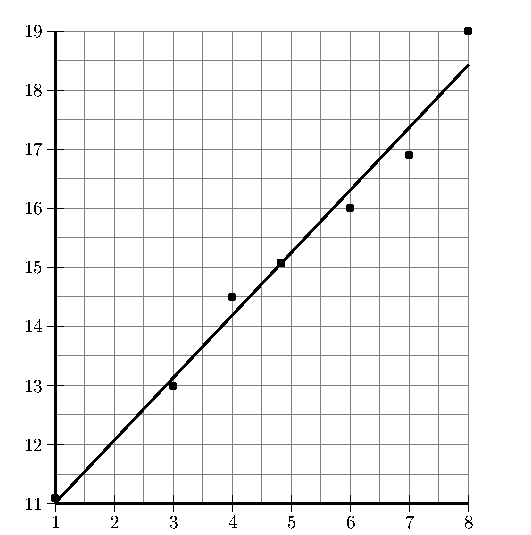
\includegraphics[scale=1]{corr_figure1.pdf} 
\end{center}
\item $\overline{x}=4,83$ \hspace*{0.2cm};\hspace*{0.2cm}$\overline{y}=15,8$
\item $y=1,06x+9,95$
\end{enumerate}
\end{corrige}

\begin{corrige}
\begin{enumerate}
\item $y=0,12x+7,84$
\item Si $x=75$, $y\approx 16,8$
\end{enumerate}
\end{corrige}

\begin{corrige}
\begin{enumerate}
\item ~ \\\begin{tabular}{|c|c|c|c|c|}
\hline Année & 1850 & 1900 & 1950 & 1990 \\ 
\hline Rang de l'année : $ x_{i} $ & 0 & 50 & 100 & 140 \\ 
\hline Teneur en $\mathrm{CO_{2}} $ : $ y_{i} $ & 275 & 290 & 315 & 360 \\ 
\hline $ z_{i}=\log (y_{i}-250) $ & 1,398 & 1,602 & 1,813 & 2,041 \\ 
\hline 
\end{tabular}
\item $z=0,004537x+1,3846$
\item 2050 correspond à $x=200$.\\
On a alors $z \approx 0,004537 \times 200 +1,3846 \Leftrightarrow \log (y-250) \approx 2,292 \Leftrightarrow y-250 \approx 10^{2,292} $\\$\Leftrightarrow y \approx 250+10^{2,292} \approx 446 $
\end{enumerate}
\end{corrige}

\begin{corrige}
\begin{enumerate}
\item Non.
\item ~\\
\begin{center}
\begin{tabular}{|c|c|c|c|c|c|}
\hline Année & 2014 & 2015 & 2016 & 2017 & 2018 \\ 
\hline Rang de l'année $ x_{i} $ & 1 & 2 & 3 & 4 & 5 \\ 
\hline Nombre d'abonnés $ y_{i} $ (en milliers) & 40 & 80 & 130 & 260 & 420 \\ 
\hline $ z_{i}=\log y_{i} $  & 4,602 & 4,903 & 5,114 & 5,415 & 5,623 \\ 
\hline 
\end{tabular} 
\end{center}
\item ~ \\
\begin{center}
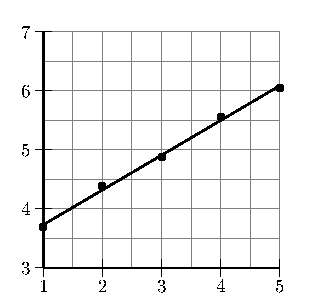
\includegraphics[scale=1]{corr_figure2.pdf} 
\end{center}
\item $z=0,255x+4,365$
\item $\log y=0,255x+4,365 \Leftrightarrow y=10^{0,255x+4,365}=10^{0,255x} \times 10^{4,365}  \approx 23,173 \times 10^{0,255x} $
\item 2022 correspond à $x=9$. \\
On a alors $y \approx 23,173 \times 10^{0,255 \times 9} \approx 4570$ milliers d'abonnés.
\end{enumerate}
\end{corrige}

\end{document}
